\documentclass[a4paper,12pt,twoside]{article}
%DIF LATEXDIFF DIFFERENCE FILE
%DIF DEL doc/sed/v1.1.1/main.tex   Fri Mar  9 00:08:48 2018
%DIF ADD doc/sed/v1.1.2/main.tex   Mon Mar 12 05:13:04 2018
\usepackage[utf8]{inputenc}
\usepackage[english]{babel}
\renewcommand\familydefault{\sfdefault}
% \usepackage[backref=true,backend=biber,hyperref=true]{biblatex}
% \bibliography{help}
\usepackage[hidelinks,bookmarksnumbered,colorlinks]{hyperref}
\hypersetup{
  colorlinks = black
  citecolor=true}
  

%\usepackage[none]{hyphenat}
\usepackage{float}
%\usepackage{subfig} Removed this bc it overrides the subcaption one, if it caused problems for anyone contact me // Lucas
\usepackage{graphicx}
%\graphicspath{} Always search for images in this folder. Dont need to add foldername in includegraphics.
\usepackage{csquotes}
\usepackage{caption}
\usepackage{subcaption}
\usepackage{amsmath}
\usepackage{ae}
\usepackage{boldline}
\usepackage{units}
%\usepackage{lscape}
\usepackage{pdflscape}
\usepackage{enumitem}
\usepackage{booktabs}
\usepackage{icomma}
\usepackage{color}
\usepackage{eurosym}
\usepackage{bbm}
\usepackage{multicol}
\usepackage{multirow}
%\usepackage{listings}
\usepackage{color}
\usepackage{verbatim}
\usepackage{wrapfig}
\usepackage[table]{xcolor}
\usepackage[utf8]{inputenc}
\usepackage{mathtools}
\usepackage{amsmath}
\usepackage[square,sort,comma,numbers]{natbib} % (tar bort konstigt fel från \usepackage{natbib})
\usepackage{textcomp}
\usepackage{siunitx}
\usepackage{pdfpages,picture} %
\usepackage{listings}
%DIF 48c48
%DIF < \usepackage{pdfpages} %Use \includepdf[pages={#,#,#,#,#}]{myfile.pdf}
%DIF -------
\usepackage[final]{pdfpages} %Use \includepdf[pages={#,#,#,#,#}]{myfile.pdf} %DIF > 
%DIF -------
%To be clear, you need to specify the pages you wish to include, i.e. \includepdf[pages={1,3,5}]{myfile.pdf} would include pages 1, 3, and 5 of the file. To include the entire file, you specify pages={-}, where {-} is a range without the endpoints specified which default to the first and last pages, respectively. The first two things I had to also do were to scale and to reenable my outer page design (to show page numbers again) which can both be set using the configuration, e.g.: \includepdf[pages=-,scale=.8,pagecommand={}]{file}
\usepackage{hyperref}
\usepackage{enumitem}
\usepackage{amsfonts}
\usepackage{afterpage}
\usepackage{longtable}
\usepackage{tabularx} %Extended tabular
\usepackage{ltxtable}
\usepackage{booktabs}
\usepackage{fancyhdr}
\usepackage{gensymb}
\usepackage{parskip} %% Vince added this to standardize paragraph spacing
\usepackage{textcomp}
\usepackage{lastpage,lipsum} %% lipsum for dummy text remove in your file
\usepackage[margin=3cm]{geometry}
\usepackage{xfrac}
\usepackage{array}
\usepackage{filecontents}
\usepackage{etoolbox}
\usepackage{nameref}
\usepackage{ragged2e}
\usepackage{enumitem}
\usepackage{xcolor}
\usepackage{pdfpages}
\usepackage{appendix}
\usepackage{spreadtab} %% Vince added this to test table sum function [2017-01-25, 15:27]

\newcolumntype{P}[1]{>{\centering\arraybackslash}p{#1}}
\newcolumntype{M}[1]{>{\centering\arraybackslash}m{#1}}
% % For references
% %\bibliographystyle{plain}
% \usepackage[numbib]{tocbibind}
% %\usepackage[nottoc]{tocbibind}
% \usepackage[paper=A4,pagesize]{typearea}    %% For putting in A3 / Hannah
%%%%%%%%%%%%%%% to be able to higlight text, for PDR update %%%%%%%%%%%%%%
\usepackage{soul} %/Hannah 
% %%%%%%%%%%%%%%%%%%%%%%%%%%%%%%%%%%%%%%%%%%%%%%%%%%%%%%%%%%%%%%%%%%%%%%%%%%%%%%%
% \usepackage[acronym]{glossaries} %natalie added 13/01/18
% \makeglossaries
% \usepackage[nopostdot]{glossaries}
\usepackage[xindy,toc]{glossaries} %natalie added 14/01/18
\makeglossaries
\usepackage[xindy]{imakeidx}
\makeindex
\usepackage{makecell} % natalie added 15/01/18 this lets you put breaks inside table boxes :3

\DeclareCaptionType[fileext=ext]{Test}
%\newfloat{Test}{luc}{Test}

%%%%%%%%%%%%%%%%%%%%%%%%%%%%%%%%%%%%%%%%%%%%%%%%%%%%%%%%%%%%%%%%%%%%%%%%%%%%%%%%%%%%%%%%%%%%%%
%%                                                                                         %%%
%%               DO NOT CHANGE IN TEX BELOW (that is literally all i have done/robo)      %%%
%%                                                                                         %%%
%%%%%%%%%%%%%%%%%%%%%%%%%%%%%%%%%%%%%%%%%%%%%%%%%%%%%%%%%%%%%%%%%%%%%%%%%%%%%%%%%%%%%%%%%%%%%%
\title{SED}
\author{tba}

\newcommand{\highlight}[1]{%
  \colorbox{yellow}{$\displaystyle#1$}}
  \makeatletter
\newcommand{\skipitems}[1]{%
  \addtocounter{\@enumctr}{#1}%
}
\makeatother
\newcommand\blankpage{%

    \null
    \thispagestyle{empty}%
    %\addtocounter{page}{-1}%
    \newpage
}
%
\fancypagestyle{SED}
{
    \fancyhf{}
    \renewcommand{\headrulewidth}{0pt}
    \chead{-\hspace{0.05cm}\thepage \hspace{0.05cm}-}
    
    %\renewcommand{\footrulewidth}{0pt}
    \fancyfoot[RE,LO]{\textit{BX26\_TUBULAR\_SEDv1-2\_12Mar18}}
    \fancyfoot[LE]{Page \thepage}
}
\fancypagestyle{cover}
{
   \fancyhf{}
   \renewcommand{\footrulewidth}{0.5pt}  
   \lfoot{\centering\textit{BX26\_TUBULAR\_SEDv1-2\_12Mar18}}
  %\cfoot{}
  % \rfoot{} 
}

\fancypagestyle{firstp}
{
    \fancyhf{}
    \renewcommand{\headrulewidth}{0pt}
   \chead{-\hspace{0.05cm}\thepage \hspace{0.05cm}-}
   \renewcommand{\footrulewidth}{0pt}  
   \fancyfoot[RE,LO]{\textit{BX26\_TUBULAR\_SEDv1-2\_12Mar18}}
   \fancyfoot[LE]{Page \thepage}
}

% \pagestyle{cover}
% \pagenumbering{roman}
%DIF PREAMBLE EXTENSION ADDED BY LATEXDIFF
%DIF UNDERLINE PREAMBLE %DIF PREAMBLE
\RequirePackage[normalem]{ulem} %DIF PREAMBLE
\RequirePackage{color}\definecolor{RED}{rgb}{1,0,0}\definecolor{BLUE}{rgb}{0,0,1} %DIF PREAMBLE
\providecommand{\DIFaddtex}[1]{{\protect\color{blue}\uwave{#1}}} %DIF PREAMBLE
\providecommand{\DIFdeltex}[1]{{\protect\color{red}\sout{#1}}}                      %DIF PREAMBLE
%DIF SAFE PREAMBLE %DIF PREAMBLE
\providecommand{\DIFaddbegin}{} %DIF PREAMBLE
\providecommand{\DIFaddend}{} %DIF PREAMBLE
\providecommand{\DIFdelbegin}{} %DIF PREAMBLE
\providecommand{\DIFdelend}{} %DIF PREAMBLE
%DIF FLOATSAFE PREAMBLE %DIF PREAMBLE
\providecommand{\DIFaddFL}[1]{\DIFadd{#1}} %DIF PREAMBLE
\providecommand{\DIFdelFL}[1]{\DIFdel{#1}} %DIF PREAMBLE
\providecommand{\DIFaddbeginFL}{} %DIF PREAMBLE
\providecommand{\DIFaddendFL}{} %DIF PREAMBLE
\providecommand{\DIFdelbeginFL}{} %DIF PREAMBLE
\providecommand{\DIFdelendFL}{} %DIF PREAMBLE
%DIF HYPERREF PREAMBLE %DIF PREAMBLE
\providecommand{\DIFadd}[1]{\texorpdfstring{\DIFaddtex{#1}}{#1}} %DIF PREAMBLE
\providecommand{\DIFdel}[1]{\texorpdfstring{\DIFdeltex{#1}}{}} %DIF PREAMBLE
\newcommand{\DIFscaledelfig}{0.5}
%DIF HIGHLIGHTGRAPHICS PREAMBLE %DIF PREAMBLE
\RequirePackage{settobox} %DIF PREAMBLE
\RequirePackage{letltxmacro} %DIF PREAMBLE
\newsavebox{\DIFdelgraphicsbox} %DIF PREAMBLE
\newlength{\DIFdelgraphicswidth} %DIF PREAMBLE
\newlength{\DIFdelgraphicsheight} %DIF PREAMBLE
% store original definition of \includegraphics %DIF PREAMBLE
\LetLtxMacro{\DIFOincludegraphics}{\includegraphics} %DIF PREAMBLE
\newcommand{\DIFaddincludegraphics}[2][]{{\color{blue}\fbox{\DIFOincludegraphics[#1]{#2}}}} %DIF PREAMBLE
\newcommand{\DIFdelincludegraphics}[2][]{% %DIF PREAMBLE
\sbox{\DIFdelgraphicsbox}{\DIFOincludegraphics[#1]{#2}}% %DIF PREAMBLE
\settoboxwidth{\DIFdelgraphicswidth}{\DIFdelgraphicsbox} %DIF PREAMBLE
\settoboxtotalheight{\DIFdelgraphicsheight}{\DIFdelgraphicsbox} %DIF PREAMBLE
\scalebox{\DIFscaledelfig}{% %DIF PREAMBLE
\parbox[b]{\DIFdelgraphicswidth}{\usebox{\DIFdelgraphicsbox}\\[-\baselineskip] \rule{\DIFdelgraphicswidth}{0em}}\llap{\resizebox{\DIFdelgraphicswidth}{\DIFdelgraphicsheight}{% %DIF PREAMBLE
\setlength{\unitlength}{\DIFdelgraphicswidth}% %DIF PREAMBLE
\begin{picture}(1,1)% %DIF PREAMBLE
\thicklines\linethickness{2pt} %DIF PREAMBLE
{\color[rgb]{1,0,0}\put(0,0){\framebox(1,1){}}}% %DIF PREAMBLE
{\color[rgb]{1,0,0}\put(0,0){\line( 1,1){1}}}% %DIF PREAMBLE
{\color[rgb]{1,0,0}\put(0,1){\line(1,-1){1}}}% %DIF PREAMBLE
\end{picture}% %DIF PREAMBLE
}\hspace*{3pt}}} %DIF PREAMBLE
} %DIF PREAMBLE
\LetLtxMacro{\DIFOaddbegin}{\DIFaddbegin} %DIF PREAMBLE
\LetLtxMacro{\DIFOaddend}{\DIFaddend} %DIF PREAMBLE
\LetLtxMacro{\DIFOdelbegin}{\DIFdelbegin} %DIF PREAMBLE
\LetLtxMacro{\DIFOdelend}{\DIFdelend} %DIF PREAMBLE
\DeclareRobustCommand{\DIFaddbegin}{\DIFOaddbegin \let\includegraphics\DIFaddincludegraphics} %DIF PREAMBLE
\DeclareRobustCommand{\DIFaddend}{\DIFOaddend \let\includegraphics\DIFOincludegraphics} %DIF PREAMBLE
\DeclareRobustCommand{\DIFdelbegin}{\DIFOdelbegin \let\includegraphics\DIFdelincludegraphics} %DIF PREAMBLE
\DeclareRobustCommand{\DIFdelend}{\DIFOaddend \let\includegraphics\DIFOincludegraphics} %DIF PREAMBLE
\LetLtxMacro{\DIFOaddbeginFL}{\DIFaddbeginFL} %DIF PREAMBLE
\LetLtxMacro{\DIFOaddendFL}{\DIFaddendFL} %DIF PREAMBLE
\LetLtxMacro{\DIFOdelbeginFL}{\DIFdelbeginFL} %DIF PREAMBLE
\LetLtxMacro{\DIFOdelendFL}{\DIFdelendFL} %DIF PREAMBLE
\DeclareRobustCommand{\DIFaddbeginFL}{\DIFOaddbeginFL \let\includegraphics\DIFaddincludegraphics} %DIF PREAMBLE
\DeclareRobustCommand{\DIFaddendFL}{\DIFOaddendFL \let\includegraphics\DIFOincludegraphics} %DIF PREAMBLE
\DeclareRobustCommand{\DIFdelbeginFL}{\DIFOdelbeginFL \let\includegraphics\DIFdelincludegraphics} %DIF PREAMBLE
\DeclareRobustCommand{\DIFdelendFL}{\DIFOaddendFL \let\includegraphics\DIFOincludegraphics} %DIF PREAMBLE
%DIF LISTINGS PREAMBLE %DIF PREAMBLE
\lstdefinelanguage{codediff}{ %DIF PREAMBLE
  moredelim=**[is][\color{red}]{*!----}{----!*}, %DIF PREAMBLE
  moredelim=**[is][\color{blue}]{*!++++}{++++!*} %DIF PREAMBLE
} %DIF PREAMBLE
\lstdefinestyle{codediff}{ %DIF PREAMBLE
	belowcaptionskip=.25\baselineskip, %DIF PREAMBLE
	language=codediff, %DIF PREAMBLE
	basicstyle=\ttfamily, %DIF PREAMBLE
	columns=fullflexible, %DIF PREAMBLE
	keepspaces=true, %DIF PREAMBLE
} %DIF PREAMBLE
%DIF END PREAMBLE EXTENSION ADDED BY LATEXDIFF

\begin{document}

%\pagenumbering{arabic}
\hypersetup{allcolors=black}

\newgeometry{left=3cm,right=2.5cm,top=1cm,bottom=3cm,headheight=20pt,headsep=10pt}
\thispagestyle{cover}


\begin{flushright}

\includegraphics[width=.25\textwidth]{0-cover/img/logo-rexus-bexus.png} 
\end{flushright}

\begin{flushright}

\begin{tabular}{p{0.70\textwidth} r}
\vspace{-1cm}
{{\hspace{-8pt}\huge{\textbf{SED}}} \vspace{15pt} \newline \vspace{15pt}
{\hspace{-11pt}\large{\textbf{Student Experiment Documentation}}} \newline \vspace{30pt}
{\hspace{-11pt}\footnotesize{Document ID: BX26\_TUBULAR\_SEDv1-2\_12Mar18}}}
& \hspace{3pt}\multirow{3}{*}{
\includegraphics[width=.25\textwidth]{0-cover/img/logo-rexus-bexus-tubular.png}}
\end{tabular}
\end{flushright}
\begin{flushleft}
\vspace{5pt}

\noindent \textbf{\hspace{-1pt}Mission: BEXUS 26} \\

\vspace{20pt}

{\hspace{-2pt}\noindent \Large{\textbf{Team Name:} } TUBULAR} \\

\vspace{20pt}

\hspace{-1pt}Experiment Title: Alternative to AirCore for Atmospheric Greenhouse Gas Sampling\\

\vspace{20pt}
\begin{tabular}{p{.33\textwidth} p{.34\textwidth} p{.33\textwidth}}
\textbf{Team} & \textbf{Name}  \\
Student Team Leader:  &  Georges L. J. Labr\`{e}che \\
\end{tabular}
\vspace{5pt}
\begin{tabular}{p{.33\textwidth} p{.34\textwidth} p{.33\textwidth}}
Team Members:  & N\'{u}ria Agues Paszkowsky \\
& Kyriaki Blazaki \\
& Jordi Coll Ortega \\
& Gustav Dyrssen \\
& Natalie Lawton \\
& Pau Molas Roca \\
& Muhammad Ansyar Rafi Putra \\
& Hamad Siddiqi \\
& Ivan Zankov \\
\end{tabular}
\begin{tabular}{p{.33\textwidth} p{.34\textwidth} p{.33\textwidth}}
University: & Lule\aa \ University of Technology
\end{tabular}

\vspace{0.5cm} 


 \begin{tabular}{p{.15\textwidth} p{.3\textwidth} p{.25\textwidth} p{.25\textwidth}}
\footnotesize{Version:}     & \footnotesize{Issue Date:} & \footnotesize{Document Type:} & \footnotesize{Valid from} \\
\textbf{1.2}          & \textbf{March 12, 2018}    & \textbf{Spec}   & \textbf{March 12, 2018} \\ 
\end{tabular}

\vspace{10pt}

\small
{
Issued by:\\
}

\vspace{0.3cm}

\large
{
\textbf{The TUBULAR Team} \\
}

\vspace{0.3cm}

\small
{
Approved by:\\
}

\vspace{0.3cm}

\large
{
\textbf{Dr. \DIFaddbegin \DIFadd{Thomas Kuhn}\\\DIFadd{Dr. }\DIFaddend Uwe Raffalski (Pending)}
}
\end{flushleft}

\newgeometry{left=2.5cm,right=2.5cm,top=2.5cm,bottom=3cm,headheight=30pt,headsep=30pt}



\pagestyle{firstp}
%\thispagestyle{firstp}
\section*{\small{\textbf{CHANGE RECORD}}}
\addcontentsline{toc}{section}{CHANGE RECORD}%

\begin{longtable}{|p{0.1\textwidth}| p{0.22\textwidth} |p{0.28\textwidth} |p{0.35\textwidth}|}\hline
    \centering
    %\begin{tabular}
    \textbf{Version}    & \textbf{Date}     & \textbf{Changed chapters} & \textbf{Remarks} \\\hline
    0       &   2017-12-20   & New Version   & Blank Book 2017  \\
    1-0     &   2018-01-15   & All           & PDR \\ 
    1-1     &   2018-01-25   & 1.1, 2.2, 2.3, 3.3.3, 3.5, 4.1, 4.4.2, 4.5, 4.6, 4.7, 6.1.5, 6.1.6, 6.2, 6.4, 7.3.1. & Incorporated feedback from supervising professor.\\ 
    1-2     &   2018-03-07   & 2.1, 2.3, 2.4, 2.5, 3.5, 4.1, 4.4, 4.6, 4.8, 5.2, 6.1.4, 6.2, 6.3, 6.4, appendix: B, C.     &    \\\hline 
    1-2     &   2018-03-08   & changed 4.5, 4.7, added 4.5.1, 4.5.2, 4.5.3, 4.5.4, 4.7.1, 4.7.2     &    \\\hline
    1-2     &   2018-03-09   & 1.5, 3.2, 3.3, 3.4, \DIFaddbegin \DIFadd{added 3.5, changed 4.1, added 5.2,  }\DIFaddend appendix: D, E, F.     & \\\hline 
    \DIFaddbegin \DIFadd{1-2     }&   \DIFadd{2018-03-11   }& \DIFadd{changed 3.2, 3.3.2, 4.1, 4.3.1, 4.4, 4.5.1, 4.5.2, 4.5.3, 4.5.4, 4.6, 4.7.1, 4.7.2, 5.2, 6.1 added 4.6.1, 4.6.2, 4.6.3, 4.6.4, appendix: F, G }&    \\\hline 
    \DIFadd{1-2     }&   \DIFadd{2018-03-12   }& \DIFadd{changed 3.1 }\\\hline 

    \DIFaddend %\end{tabular}
    \label{COR}
\end{longtable}

\vspace{1cm}
\begin{tabular}{p{.15\textwidth} p{.85\textwidth}}
\textbf{Abstract:}     &  %Document Abstract  \\
Carbon dioxide (CO$_{2}$), methane (CH$_{4}$), and nitrous oxide (N$_2$O) are three main greenhouse gases emitted by human activities. Developing a better understanding of their contribution to greenhouse effects requires more accessible, flexible, and scalable air sampling mechanisms. A balloon flight is the most cost-effective mechanism to obtain a vertical air profile through continuous sampling between the upper troposphere and the lower stratosphere. However, recovery time constraints due to gas mixture concerns geographically restrict the sampling near existing research centers where analysis of the recovered samples can take place. The TUBULAR experiment is a technology demonstrator for atmospheric research supporting an air sampling mechanism that would offer climate change researchers access to remote areas by minimizing the effect of gas mixtures within the collected samples so that recovery time is no longer a constraint. The experiment will include a secondary sampling mechanism that will serve as reference against which the proposed sampling mechanism can be validated.
  &  \\
\textbf{Keywords:}     & %Document Keywords
Balloon Experiments for University Students, Climate Change, Stratospheric Air Sampling, AirCore, Sampling Bags, Greenhouse Gas, Carbon Dioxide (CO$_{2}$), Methane (CH$_{4}$), Nitrous Oxide (N$_{2}$O).
\end{tabular}

\vfill

\newpage
\tableofcontents
%\newpage

\newpage
\section*{PREFACE} \markboth{}{}
\addcontentsline{toc}{section}{PREFACE}

The Rocket and Balloon Experiments for University Students (REXUS/BEXUS) program is realized under a bilateral Agency Agreement between the German Aerospace Center (DLR) and the Swedish National Space Board (SNSB). The Swedish share of the
payload has been made available to students from other European countries through a collaboration with the European Space Agency (ESA).

EuroLaunch, a cooperation between the Esrange Space Center of SSC and the Mobile Rocket Base (MORABA) of DLR, is responsible for the campaign management and operations of the launch vehicles. Experts from DLR, SSC, ZARM, and ESA provide
technical support to the student teams throughout the project.

The Student Experiment Documentation (SED) is a continuously updating document regarding the BEXUS student experiment TUBULAR - Alternative AirCore for Atmospheric Greenhouse Gas Sampling (TUBULAR) and will undergo reviews during the preliminary design review, the critical design review, the integration progress review, and final experiment report.

The TUBULAR Team consists of a diverse and inter-disciplinary group of students from Luleå University of Technology's Masters programme in Atmospheric Studies, Space Engineering, and Spacecraft Design. The idea for the proposed experiment stems from two concerns over the realities of climate change as a result of human activity coupled with the complexity and limitations in obtaining greenhouse gas profile data to support climate change research.

Based above the Arctic circle in Kiruna, Sweden, the TUBULAR Team is exposed to Arctic science research with which it will interact with in order to produce a research detailing the air sampling methodology, measurements, analysis, and findings.

\subsection*{File Naming}
The naming convention for the SED is as follows:
\begin{itemize}
  \item BX for BEXUS or RX for REXUS, plus number of flight
  \item Experiment name
  \item SED, plus version (e.g. 3 for CDR) and issue number (beginning with 0 and increasing number when a new issue is sent)
  \item Date of issue in format ddmmmyy
\end{itemize}
e.g. BX26\_TUBULAR\_SEDv1-0\_15Jan18.pdf


\newpage
\section*{Acknowledgements} \markboth{}{}

The TUBULAR team wishes to acknowledge the \DIFaddbegin \DIFadd{invaluable support received by the REXUS/BEXUS organizers, SNSB, DLR, ESA, SSC, ZARM, ESRANGE, and ESA Education. In particular, the team's gratitude extends to the }\DIFaddend following project advisers who show special interest in our experiment:

\begin{itemize}
  \item \textbf{Dr. \DIFdelbegin \DIFdel{Uwe Raffalski}\DIFdelend \DIFaddbegin \DIFadd{Rigel Kivi}\DIFaddend }, \DIFdelbegin \DIFdel{Associate Professor at the Swedish Institute of Space physics (IRF)and the project's endorsing professor. Dr}\DIFdelend \DIFaddbegin \DIFadd{Senior Scientist at the Finnish Meteorological Institute (FMI)}\DIFaddend . \DIFdelbegin \DIFdel{Raffalski}\DIFdelend \DIFaddbegin \DIFadd{A key project partner, Dr. Kivi}\DIFaddend 's research and experience in Arctic atmospheric studies serves as a knowledge-base reference that ensures proper design of the experiment.
  \item \textbf{Dr. \DIFdelbegin \DIFdel{Rigel Kivi}\DIFdelend \DIFaddbegin \DIFadd{Uwe Raffalski}\DIFaddend }, \DIFdelbegin \DIFdel{Senior Scientist at the Finnish Meteorological Institute (FMI) . A key projectpartner, Dr. Kivi}\DIFdelend \DIFaddbegin \DIFadd{Associate Professor at the Swedish Institute of Space physics (IRF) and the project's endorsing professor. Dr. Raffalski}\DIFaddend 's research and experience in Arctic atmospheric studies serves as a knowledge-base reference that ensures proper design of the experiment.
  \item \textbf{Dr. Thomas Kuhn}, Associate Professor at Luleå  University of Technology (LTU). A project course offered by Dr. Kuhn serves as a merited university module all while providing the team with guidance and supervision.
  \item \textbf{Mr. Olle Persson}, Operations Administrator at Luleå University of Technology (LTU). A former REXUS/BEXUS affiliate, Mr. Persson has been providing guidance based on his experience.
  \DIFaddbegin \item \textbf{\DIFadd{Mr. Grzegorz Izworski}}\DIFadd{, Electromechanical Instrumentation Engineer at European Space Agency (ESA) in the Engineering Services Section, ESTEC Test Centre Division, Mechanical Department with is within the Directorate of Tech, Eng. }& \DIFadd{Quality. Mr. Izworski is the team's mentor supporting design and development of the project to ensure launch success.
  }\item \textbf{\DIFadd{Mr. Koen Debeule}}\DIFadd{, Electronic Design Engineer at European Space Agency (ESA). Mr. Debeule is the team's supporting mentor.
}\DIFaddend \end{itemize}


\pagestyle{SED}
\newgeometry{left=2.5cm,right=2.5cm,top=2.5cm,bottom=3cm,headheight=30pt,headsep=30pt}
\raggedbottom  % Fixed random spacing in text /H

%\pagenumbering{arabic}
%\input sections

% MAIN TEXT DOCUMENT 
\section{Introduction}
\subsection{Scientific Background}

The ongoing and increasingly rapid melting of the Arctic ice cap has served as a reference to the global climate change. Researchers have noted that \enquote{the Arctic is warming about twice as fast as the rest of the world} \cite{Perkins} and projecting an ice-free Arctic Ocean as a realistic scenario in future summers similar to the Pliocene Epoch when \enquote{global temperature was only 2–3°C warmer than today} \cite{Trace}. Suggestions that additional loss of Arctic sea ice can be avoided by reducing air pollutant and CO$_{2}$ growth still require confirmation through better climate effect measurements of CO$_{2}$ and non-CO$_{2}$ forcings \cite{Trace}. Such measurements bear high costs, particularly in air sampling for trace gas concentrations in the region between the upper troposphere and the lower stratosphere which have a significant effect on the Earth's climate. There is little information on distribution of trace gases at the stratosphere due to the inherent difficulty of measuring gases above aircraft altitudes.

Trace gases, are gases which makes up less than 1\% by volume of the Earth's atmosphere. They include all gasses except Nitrogen, and Oxygen. In terms of climate change, the main concern of the scientific community, focuses on CO$_2$ and CH$_4$ which make up less than 0.1\% of the 1\%, and are referred to as Greenhouse gases. Greenhouse gas concentrations are measured in parts per million (ppm), and parts per billion (ppb). They are the main offenders of the greenhouse effect, released by human activity as they trap heat into the atmosphere. Larger emissions of greenhouse gases lead to higher concentrations of those gases in the atmosphere thus contributing to climate change.

\subsection{Mission Statement}

There is little information on distribution of trace gases at the stratosphere due to the inherent difficulty and high cost of air sampling above aircraft altitudes \cite{Trace}. The experiment seeks to contribute to and support climate change research by proposing and validating a low-cost air sampling mechanism that reduces the current complexities and limitations of obtaining data on stratospheric greenhouse gas distribution.
\pagebreak
\subsection{Experiment Objectives}

Beyond providing knowledge on greenhouse gas distributions, the sampling obtained from the experiment will serve as a reference to validate the robustness and reliability of proposed sampling system through comparative analysis of results obtained with a reference sampling system.

The primary objective of the experiment consists of validating the proposed sampling system as a reliable mechanism that enables sampling of stratospheric greenhouse gases in remote areas.

The secondary objective of the experiment will be to analyze the samples by both systems in a manner that will contribute to climate change research in the Arctic region. The trace gas profiles to be analyzed are that of carbon dioxide (CO$_{2}$), methane (CH$_{4}$), and nitrous oxide (N$_{2}$O). 
\subsection{Experiment Concept}

The experiment seeks to test the viability and reliability of a proposed cost-effective alternative to the The AirCore Sampling System. The AirCore Sampling System consists of a long and thin stainless steel tube shaped in the form of a coil which takes advantage of changes in pressure during descent to sample the surrounding atmosphere and preserve a profile (see Figure \ref{fig:A1} in Appendix A). Sampling during a balloon’s descent phase will result in a profile shape extending the knowledge of distribution of trace gases for the measured column between the upper troposphere and the lower stratosphere \cite{Karion}. The proposed experiment will consist of two sampling subsystems: a conventional implementation of AirCore as described above, henceforth referred to as CAC, and a proposed alternative, henceforth referred to as Alternative AirCore (AAC).

The proposed AAC system is primarily motivated by the CAC sampling mechanism lacking flexibility in choice of coverage area due to the geographical restriction imposed by the irreversible process of gas mixing along the air column sampled in its stainless tube. Because of this, the sampling region for the CAC system needs to remain within proximity to research facilities for post-flight gas analysis. The AAC sampling system is a proposed alternative configuration to the CAC sampling system that has been designed to address this limitation all while improving cost-effectiveness. The AAC sampling system consists of a series of small independent air sampling bags (see Figure \ref{fig:A2} in Appendix A) rather than a single long tube as for the CAC. The air sampling bags will be opened and closed in series to ensure continuous sampling in which analysis can then be merged into a single profile. Each sampling bag is to be allocated a small vertical sampling size of 500 meters in which mixing of gases becomes a lesser concern.

The use of sampling bags in series rather than a single long tube is meant to tackle limitations of CAC by 1) reducing system implementation cost inherent to the production of a long tube and 2) enabling sampling of remote areas by reducing the effect of mixing of gases in post-analysis. Overall design of AAC will be approached with miniaturization, cost-effectiveness, and design for manufacturability (DFM) in mind with the purpose of enabling ease of replication.
\pagebreak
\subsection{Team Details}
The TUBULAR team consists of diverse and inter-disciplinary team members 

\bigskip


\begin{longtable}[]{m{0.25\textwidth} m{0.6\textwidth}}

 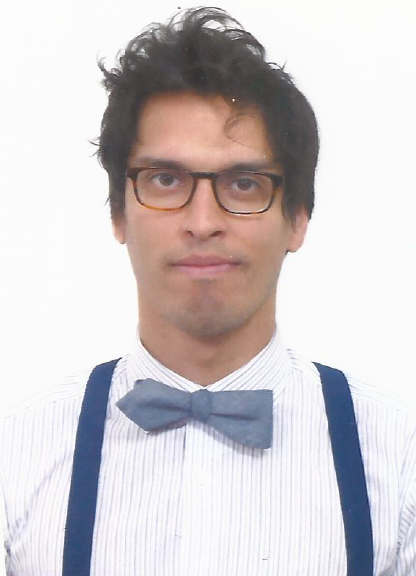
\includegraphics[width=0.2\textwidth]{1-introduction/img/georges-louis-joseph-labreche.jpg}  & \textbf{Georges L. J. Labrèche - Management Division}

\smallskip
\textit{Education}: BSc in Software Engineering with experience in technical leadership and project management in software development.

\smallskip
\textit{Responsibilities}: Acting as Systems Engineer and managing overall implementation of the project. Establishing and overseeing product development cycle. Coordinating between different teams, project stakeholders, and documentation efforts.                          
\bigskip
\\

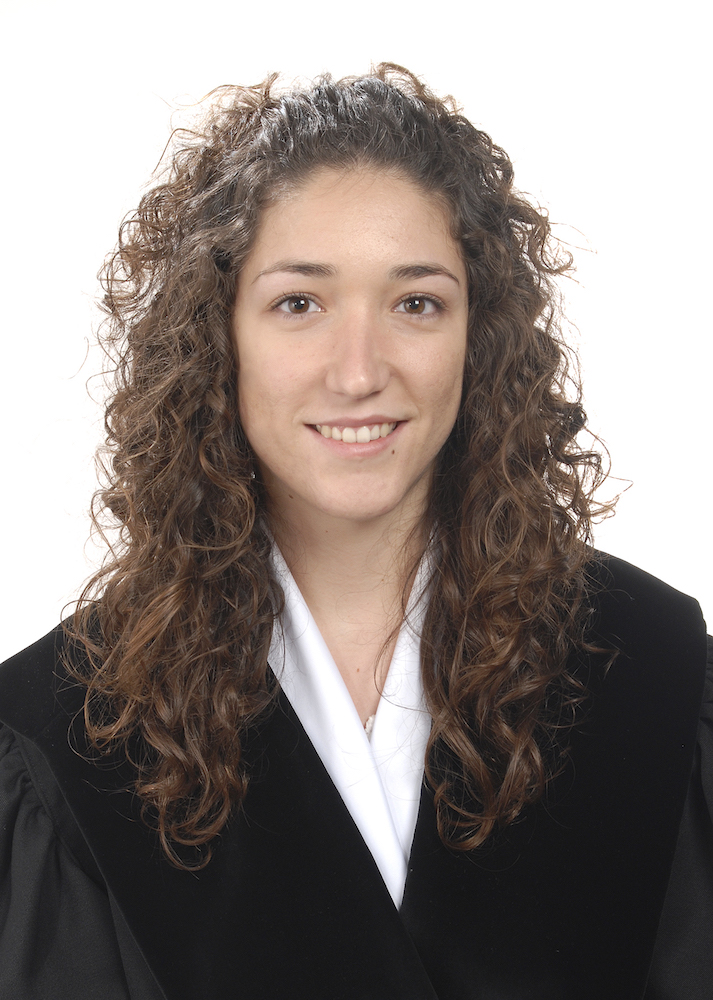
\includegraphics[width=0.2\textwidth]{1-introduction/img/agues-paszkowsky.jpg} & \textbf{Nuria Agües Paszkowsky - Scientific Division}

\smallskip
\textit{Education}: BSc in Aerospace Engineering.

\smallskip
\textit{Responsibilities}: Defining experiment parameters; data analysis; interpreting and documenting measurements; research on previous AirCore experiments for comparative analysis purposes; contacting researchers or institutions working on similar projects; exploring potential partnership with researchers and institutions, evaluating the reliability of the proposed AAC sampling system; conducting measurements of collected samples; documenting and publishing findings. 
\bigskip
\\

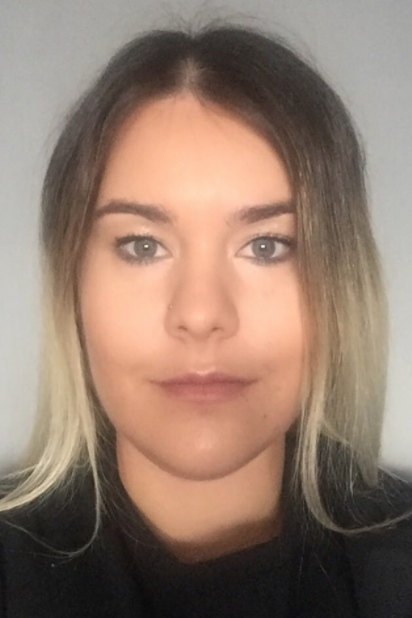
\includegraphics[width=0.2\textwidth]{1-introduction/img/kiki-blazaki.jpg} & \textbf{Kyriaki Blazaki - Scientific Division}

\smallskip
\textit{Education}: BSc in Physics.


\smallskip
\textit{Responsibilities}: Coordinating between the team and the Project Manager; defining experiment parameters; data analysis; interpreting and documenting measurements; research on previous AirCore experiments for comparative analysis purposes; evaluating the reliability of the proposed AAC sampling system; conducting measurements of collected samples; documenting and publishing findings. 
\bigskip
\\

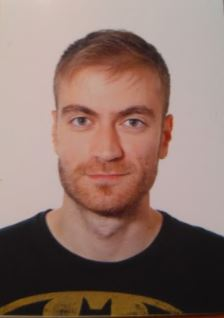
\includegraphics[width=0.2\textwidth]{1-introduction/img/jordi-coll-ortega.jpg} & \textbf{Jordi Coll Ortega - Mechanical Division}

\smallskip
\textit{Education}: BASc in Aerospace Vehicle Engineering.

\smallskip
\textit{Responsibilities}: Designing or redesigning cost-effective mechanical devices using analysis and computer-aided design; developing and testing prototypes of designed devices; analyzing the test results and changing the design as needed in collaboration with the team lead; integrating and assembling final design.
\bigskip
\\

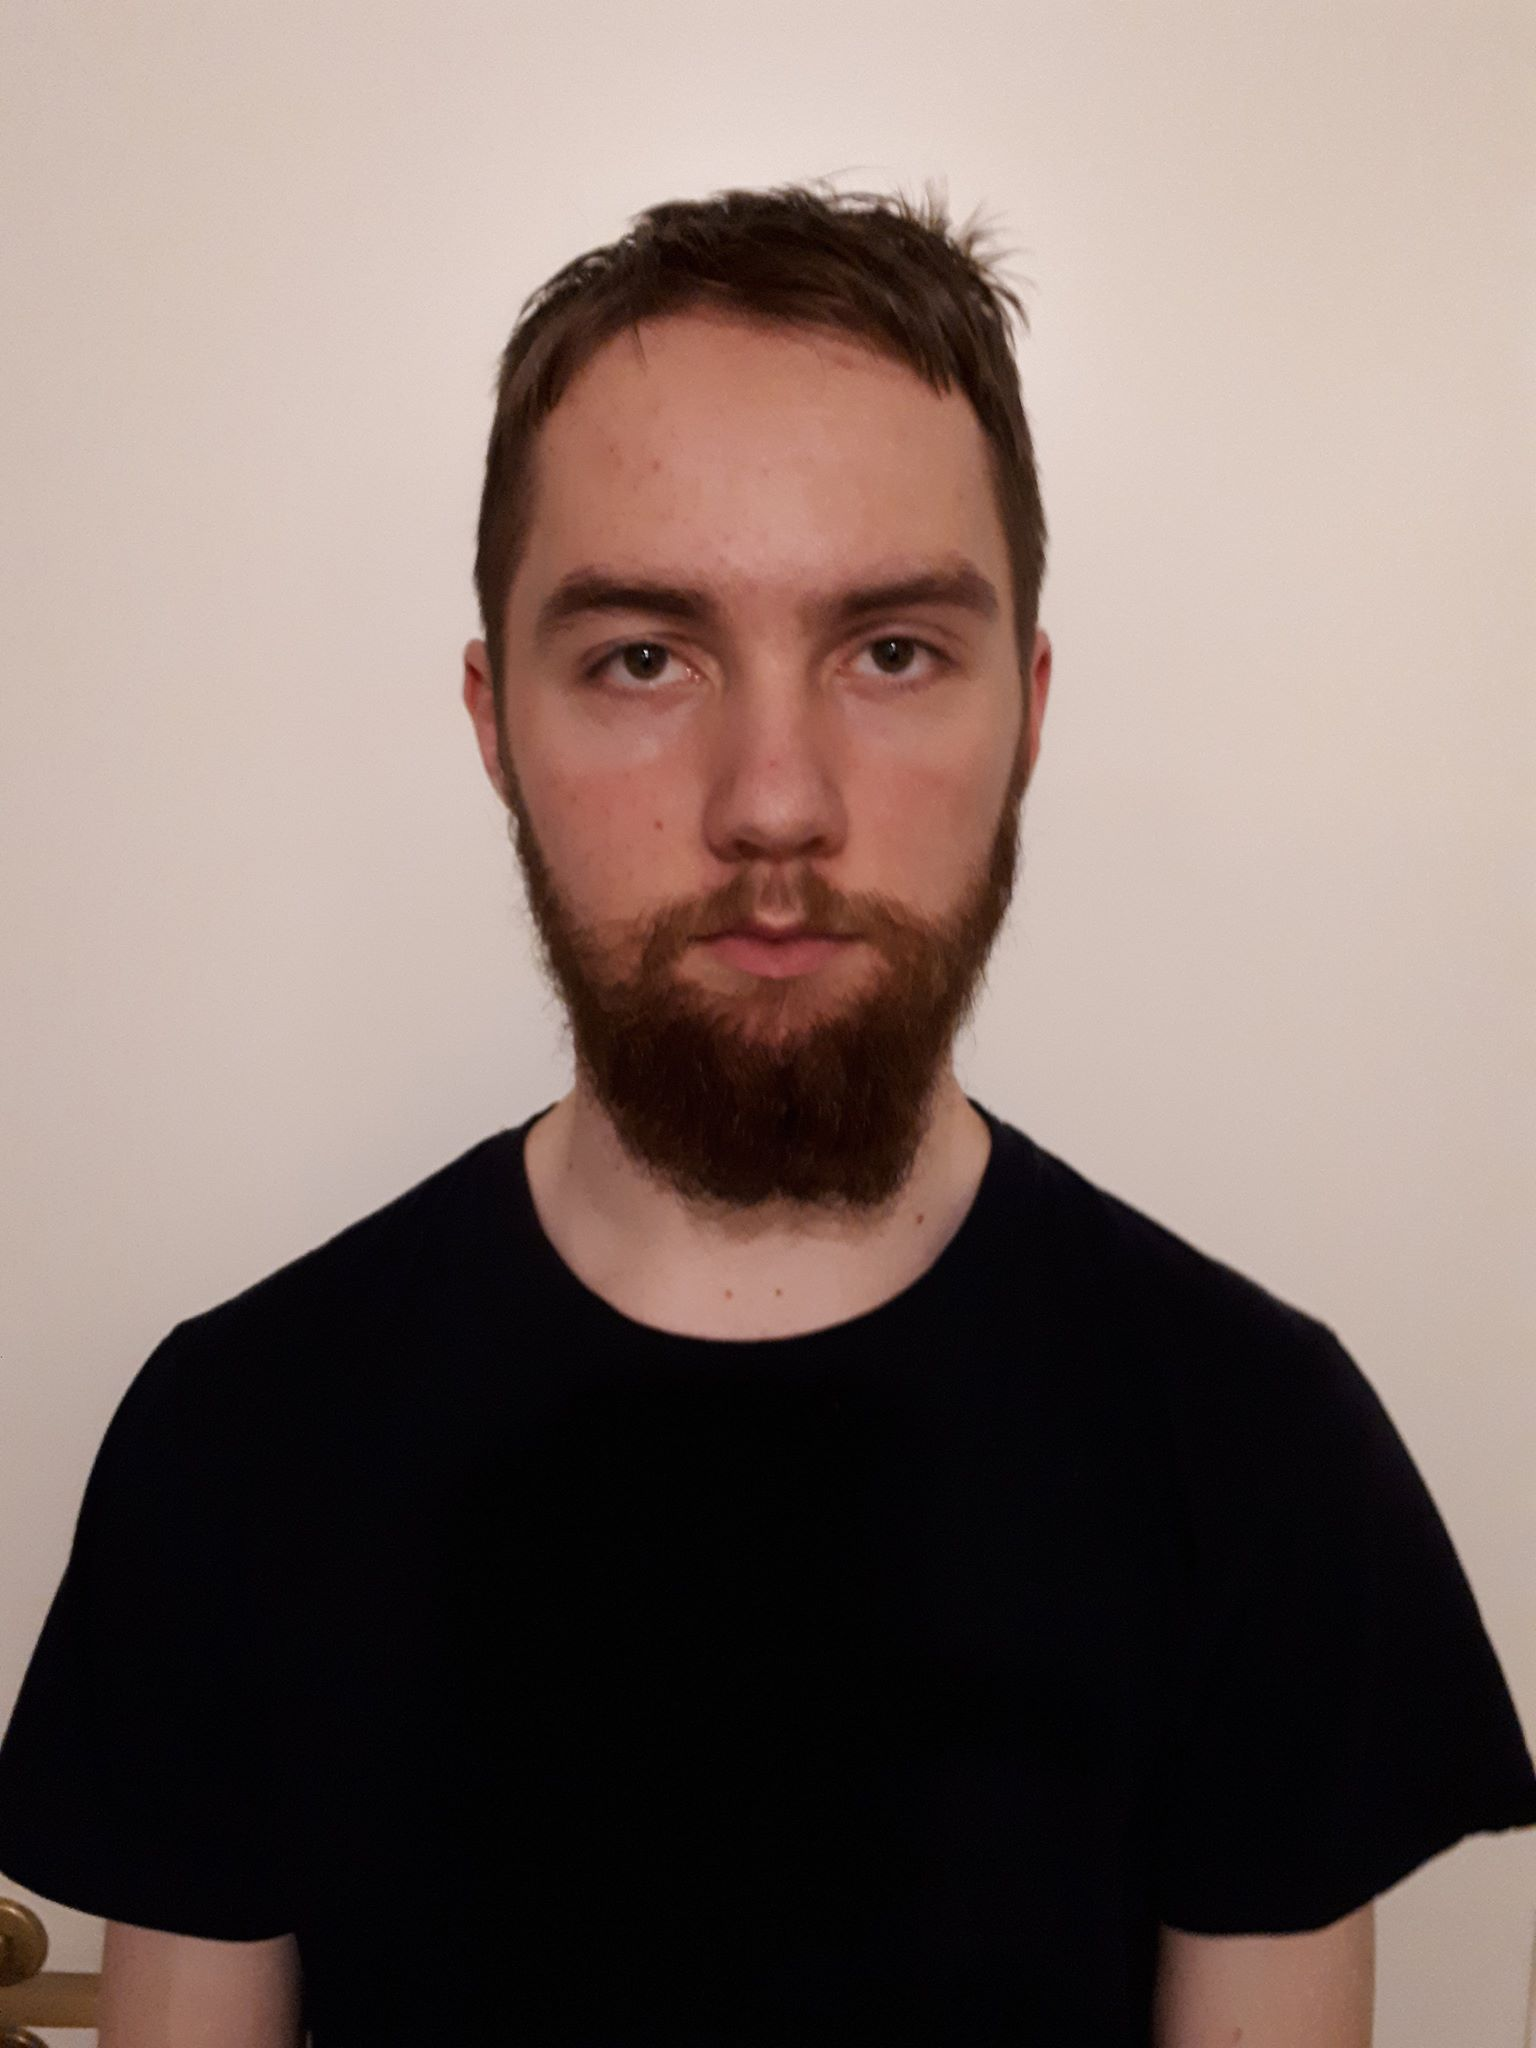
\includegraphics[width=0.2\textwidth]{1-introduction/img/gustav-dryssen.jpg} & \textbf{Gustav Dyrssen - Software Division}

\smallskip
\textit{Education}: MSc in Space Engineering (4th Year).

\smallskip
\textit{Responsibilities}: Leading quality assurance and testing efforts; Enforcing software testing best practices such as continuous integration testing and regression testing; reviewing requirements and specifications in order to foresee potential issues; provide input of functional requirements; advising on design; formalizing test cases; tracking defects and ensuring their resolution; facilitating code review sessions; supporting software implementation efforts.     
\bigskip
\\


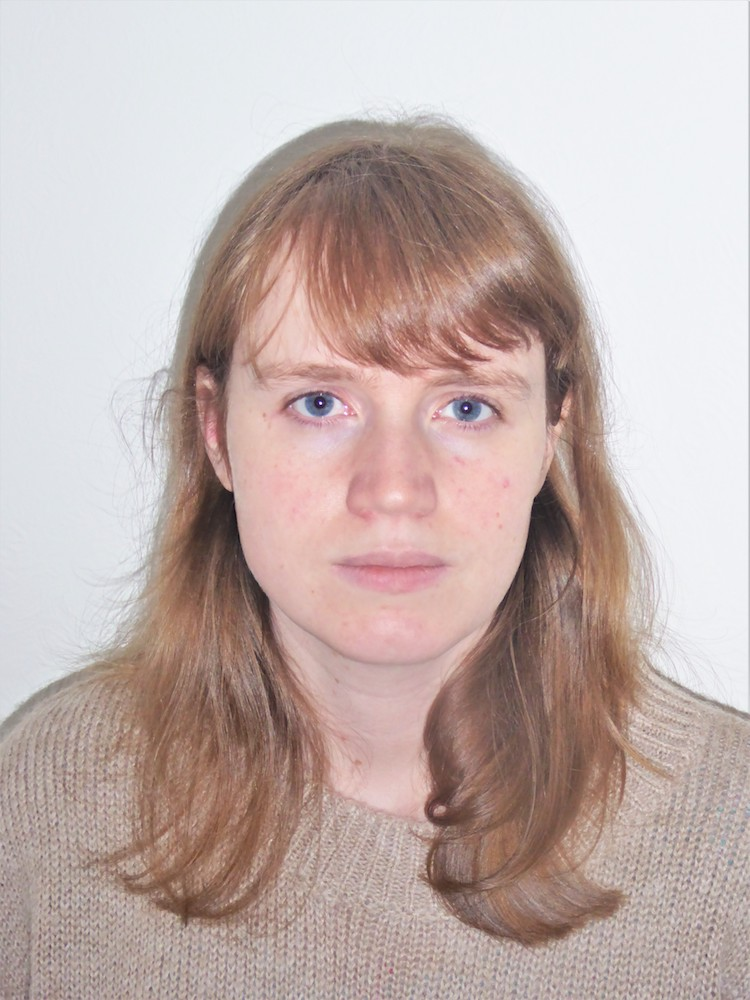
\includegraphics[width=0.2\textwidth]{1-introduction/img/natalie-lawton.jpg} & \textbf{Natalie Lawton - Electrical Division}

\smallskip
\textit{Education}: MEng in Aerospace Engineering. Previous experience in UAV avionic systems and emissions measurement techniques.

\smallskip
\textit{Responsibilities}: Supporting designing and implementing cost-effective circuitry using analysis and computer-aided design; Reviewing and testing proposed designs; recommending modifications following prototype test results; assembling designed circuitry. 
\bigskip
\\

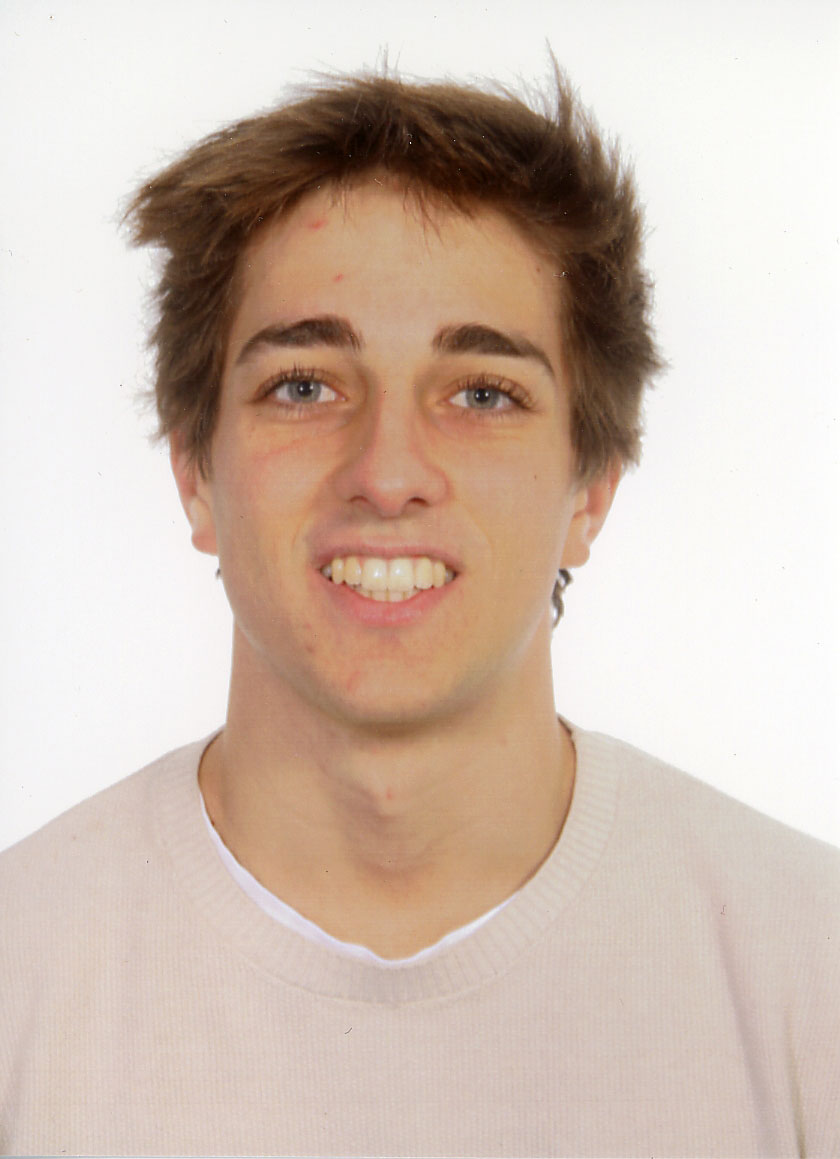
\includegraphics[width=0.2\textwidth]{1-introduction/img/pau-molas-roca.jpg} & \textbf{Pau Molas Roca - Mechanical Division}

\smallskip
\textit{Education}: BSc in Aerospace Technology Engineering, Mechanical experience.

\smallskip
\textit{Responsibilities}: Coordinating between the team and the Project Manager; designing or redesigning cost-effective mechanical devices using analysis and computer-aided design; producing details of specifications and outline designs; overseeing the manufacturing process for the devices; identifying material and component suppliers; integrating and assembling final design.   \bigskip
\\

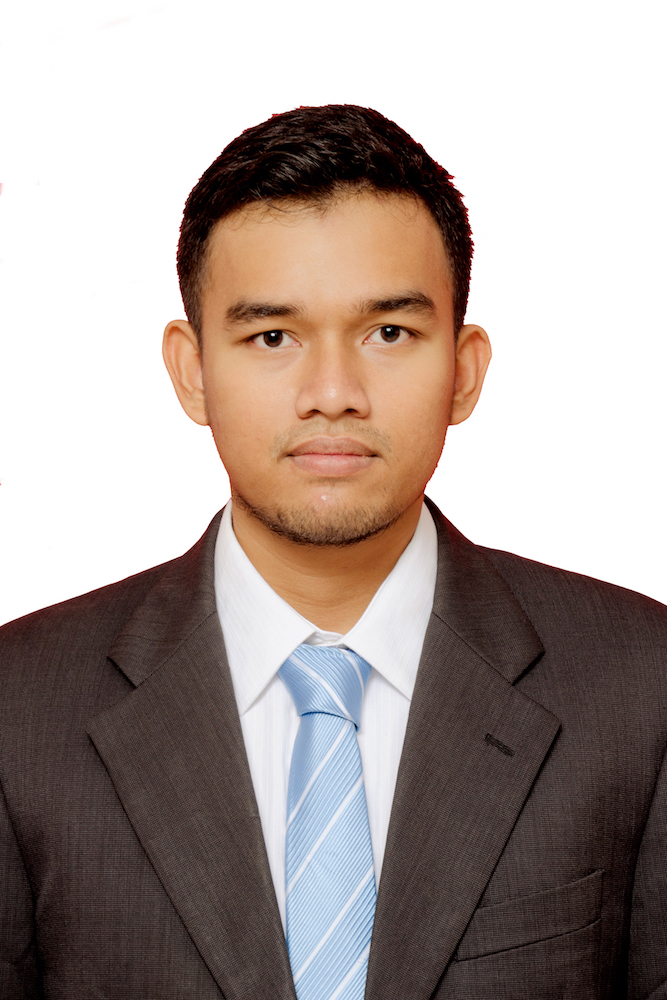
\includegraphics[width=0.2\textwidth]{1-introduction/img/muhammad-ansyar-rafi-putra.jpg} & \textbf{Muhammad Ansyar Rafi Putra - Software Division}

\smallskip
\textit{Education}: BSc in Aerospace Engineering.


\smallskip 
\textit{Responsibilities}: Coordinating between the team and the Project Manager; gathering software requirements; formalizing software specifications; drafting architecture design, detailed design; leading software implementation efforts.
\bigskip
\\

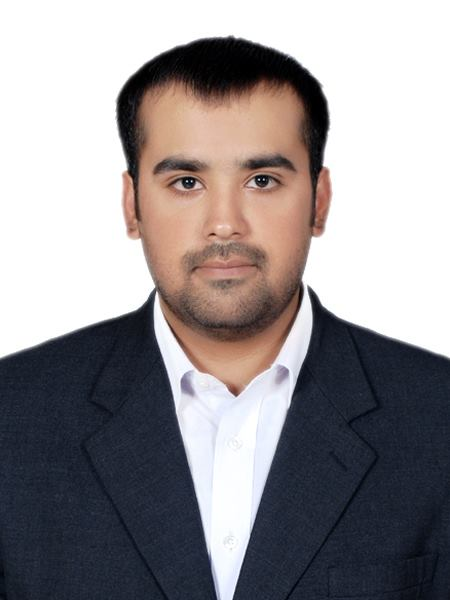
\includegraphics[width=0.2\textwidth]{1-introduction/img/hamad-saddiqi.jpg} & \textbf{Hamad Siddiqi - Electrical Division}

\smallskip
\textit{Education}: BSc in Electrical Engineering with experience in telecommunication industry and electronics.

\smallskip
\textit{Responsibilities}: Coordinating between the team and the Project Manager; designing and implementing cost-effective circuitry using analysis and computer-aided design; producing details of specifications and outline designs; developing, testing, and evaluating theoretical designs; identifying material as well as component suppliers. 
\bigskip
\\


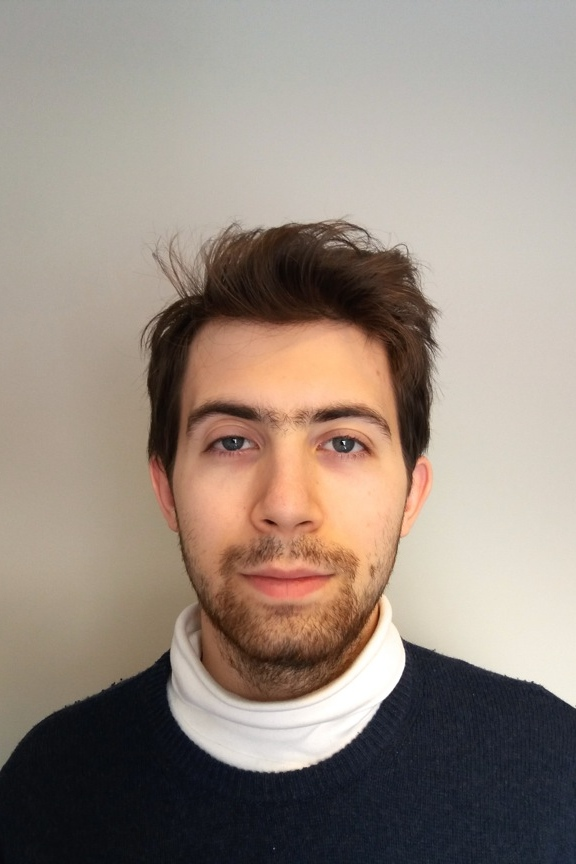
\includegraphics[width=0.2\textwidth]{1-introduction/img/ivan-zankov.jpg} & \textbf{Ivan Zankov - Thermal Division}

\smallskip
\textit{Education}: BEng in Mechanical Engineering.

\smallskip
\textit{Responsibilities}: Thermal analysis of proposed designs and Recommending modifications following thermal analysis results..                                                          

\\
\label{tab:people}
\end{longtable}
\raggedbottom

\pagebreak
\section{Experiment Requirements and Constraints}

\subsection{Functional Requirements}

\begin{enumerate}
    \item[F.1] \st{The experiment \textit{shall} collect air samples.}\footnote{Unnecessary requirement that has been removed.\label{fn:unnecessary-requirement}}
    \item[F.2] The experiment \textit{shall} collect air samples by the CAC.
    \item[F.3] The experiment \textit{shall} collect air samples by the AAC.
    \item[F.4] \st{The experiment's AAC System \textit{shall} be able to collect air samples during the ascent phase.}\textsuperscript{\ref{fn:unnecessary-requirement}}
    \item[F.5] \st{The experiment's AAC System \textit{shall} be able to collect air samples during the descent phase.}\textsuperscript{\ref{fn:unnecessary-requirement}}
    \item[F.6] The altitude from which a sampling bag will start sampling \textit{shall} be programmable.
    \item[F.7] The altitude from which a sampling bag will stop sampling \textit{shall} be programmable.
    \item[F.8] \st{The experiment \textit{shall} pump air into the AAC Sampling Bags.}\textsuperscript{\ref{fn:unnecessary-requirement}}
    \item[F.9] The experiment \textit{should} collect data on the air intake flow to the AAC.
    \item[F.10] The experiment \textit{shall} collect data on the air pressure.
    \item[F.11] The experiment \textit{shall} collect data on the temperature.
    \item[F.12] The experiment \textit{shall} collect data on the humidity.
    \item[F.13] \st{The experiment \textit{shall} measure the temperature inside the AAC Valve Box.}\textsuperscript{\ref{fn:unnecessary-requirement}}
    \item[F.14] \st{The experiment \textit{should} measure the humidity inside the AAC Valve Box.}\textsuperscript{\ref{fn:unnecessary-requirement}}
    \item[F.15] \st{The experiment \textit{shall} collect data on the time.}\footnote{Unverifiable requirement that has been removed.\label{fn:unverifiable-requirement}}
    \item[F.16] \st{The experiment \textit{shall} accept telecommand instructions to program AAC sampling altitudes for each sampling bag.}\textsuperscript{\ref{fn:unnecessary-requirement}}
    \item[F.17] \st{The experiment \textit{shall} accept telecommand instructions to open designated valves.}\textsuperscript{\ref{fn:unnecessary-requirement}}
    \item[F.18] \st{The experiment \textit{shall} accept telecommand instructions to close designated valves.}\textsuperscript{\ref{fn:unnecessary-requirement}}
    \item[F.19] \st{The experiment \textit{may} accept telecommand instructions to change the sampling rate of the ambient pressure sensor.}\textsuperscript{\ref{fn:unnecessary-requirement}}
    \item[F.20] \st{The experiment \textit{may} accept telecommand instructions to change the sampling rate of the ambient temperature sensor.}\textsuperscript{\ref{fn:unnecessary-requirement}}
    \item[F.21] \st{The experiment \textit{may} accept telecommand instructions to change the sampling rate of the AAC Valve Box temperature sensor.}\textsuperscript{\ref{fn:unnecessary-requirement}}
    \item[F.22] \st{The experiment \textit{may} accept telecommand instructions to turn on the air pump.}\textsuperscript{\ref{fn:unnecessary-requirement}}
    \item[F.23] \st{The experiment \textit{may} accept telecommand instructions to turn off the air pump.}\textsuperscript{\ref{fn:unnecessary-requirement}}
    \item[F.24] \st{The experiment \textit{may} accept telecommand instructions to turn on the Valve Heater.}\textsuperscript{\ref{fn:unnecessary-requirement}}
    \item[F.25] \st{The experiment \textit{may} accept telecommand instructions to turn off the Valve Heater.}\textsuperscript{\ref{fn:unnecessary-requirement}}
    \item[F.26] \st{The experiment \textit{may} accept telecommand instructions to turn on the Electronics Box Heater.}\textsuperscript{\ref{fn:unnecessary-requirement}}
    \item[F.27] \st{The experiment \textit{may} accept telecommand instructions to turn off the Electronics Box Heater.}\textsuperscript{\ref{fn:unnecessary-requirement}}
\end{enumerate}
\pagebreak
\subsection{Performance Requirements}

\begin{enumerate}[label=P.\arabic*]
    \item \st{The telecommand data rate \textit{shall} be 10Kb/s.}\footnote{Moved to design requirements.\label{fn:design-requirement}}
    \item \st{The default sampling rate of the ambient pressure sensor during Standby mode \textit{shall} be 0.1 Hz.}\footnote{Replaced by \ref{newsamplerate}\label{replaceSampleRate}}
    \item \st{The default sampling rate of the ambient pressure sensor during Normal operation-ascent mode \textit{shall} be 0.2 Hz.}\textsuperscript{\ref{replaceSampleRate}}
    \item \st{The default sampling rate of the ambient pressure sensor during Normal operation-descent mode \textit{shall} be 10 Hz.}\textsuperscript{\ref{replaceSampleRate}}
    %\item The default sampling rate of the ambient pressure sensor \textit{shall} be TBD.
    \item \st{The default sampling rate of the AAC Valve Box temperature sensor \textit{shall} be 1 Hz.}\textsuperscript{\ref{replaceSampleRate}}
    \item \st{The programmable sampling rate of the ambient pressure sensor \textit{shall} not be lesser than 0.1 Hz.}\textsuperscript{\ref{replaceSampleRate}}
    \item \st{The programmable sampling rate of the ambient pressure sensor \textit{shall} not be greater than 100 Hz.}\textsuperscript{\ref{replaceSampleRate}}
    \item \st{The programmable sampling rate of the Electronics Box temperature sensor \textit{shall} not be lesser than 1Hz.}\textsuperscript{\ref{replaceSampleRate}}
    \item \st{The programmable sampling rate of the Electronics Box temperature sensor \textit{shall} not be greater than 7Hz.}\textsuperscript{\ref{replaceSampleRate}}
    \item \st{The programmable sampling rate of the AAC Valve Box temperature sensor \textit{shall} not be lesser than 1 Hz.}\textsuperscript{\ref{replaceSampleRate}}
    \item \st{The programmable sampling rate of the AAC Valve Box temperature sensor \textit{shall} not be greater than 7 Hz.}\textsuperscript{\ref{replaceSampleRate}}
    %\item The programmable sampling rate of the pressure sensor \textit{shall} not be lesser than .
    \item The accuracy of the ambient pressure measurements \textit{shall} be -1.5/+1.5 mbar for 25$\degree$C.
    \item The accuracy of \DIFdelbegin \DIFdel{the Electronics Box }\DIFdelend temperature measurements \textit{shall} be +3.5/-2$\degree$C (max) for condition of -55$\degree$C to 150$\degree$C.
    \item The accuracy of the ambient humidity measurements \textit{shall} be ±3 percent. \cite{Humiditysensor}
    \item \DIFdelbegin \DIFdel{The accuracy of the AAC Valve Box temperature measurements }\textit{\DIFdel{shall}} %DIFAUXCMD
\DIFdel{be +3.5/-2°C(max).
    }\DIFdelend \DIFaddbegin \st{The accuracy of the AAC Valve Box temperature measurements \textit{shall} be +3.5/-2°C(max).}\footnote{\DIFadd{Combined with P13}}
    \DIFaddend \item The air intake rate of the air pump \textit{shall} be minimum 3L/min.
    \item The temperature of the Electronics Box \textit{shall} \DIFdelbegin \DIFdel{not go below }\DIFdelend \DIFaddbegin \DIFadd{be between }\DIFaddend 0$\degree$C \DIFdelbegin \DIFdel{.
    }%DIFDELCMD < \item %%%
\item%DIFAUXCMD
\DIFdel{The temperature of the Electronics Box }\textit{\DIFdel{shall}} %DIFAUXCMD
\DIFdel{not exceed }\DIFdelend \DIFaddbegin \DIFadd{and }\DIFaddend 25$\degree$C.
    \item \DIFaddbegin \st{The temperature of the Electronics Box \textit{shall} not exceed 25\mbox{%DIFAUXCMD
$\degree$
}%DIFAUXCMD
C.}\footnote{\DIFadd{Combined with P17}}
    \item \DIFaddend The temperature of the AAC Valve Box \textit{shall} \DIFdelbegin \DIFdel{not go below }\DIFdelend \DIFaddbegin \DIFadd{be between }\DIFaddend 0$\degree$C \DIFdelbegin \DIFdel{.
    }%DIFDELCMD < \item %%%
\item%DIFAUXCMD
\DIFdel{The temperature of the AAC Valve Box }\textit{\DIFdel{shall}} %DIFAUXCMD
\DIFdel{not exceed }\DIFdelend \DIFaddbegin \DIFadd{and }\DIFaddend 25$\degree$C.
    \item \DIFdelbegin \DIFdel{The AAC air sampling }\DIFdelend \DIFaddbegin \st{The temperature of the AAC Valve Box \textit{shall} not exceed 25\mbox{%DIFAUXCMD
$\degree$
}%DIFAUXCMD
C.}\footnote{\DIFadd{Combined with P19}}
    \item \DIFadd{The air sampling systems }\DIFaddend \textit{shall} filter out all water molecules before filling the sampling \DIFdelbegin \DIFdel{bags}\DIFdelend \DIFaddbegin \DIFadd{containers}\DIFaddend .
    \item \DIFdelbegin \DIFdel{The CAC air sampling }\textit{\DIFdel{shall}} %DIFAUXCMD
\DIFdel{filter out all water molecules before filling the tube.
    }\DIFdelend \DIFaddbegin \st{The CAC air sampling \textit{shall} filter out all water molecules before filling the tube.}\footnote{\DIFadd{Combined with P21}}
    \DIFaddend \item The \DIFaddbegin \DIFadd{sensors }\DIFaddend sampling rate \textit{shall} be 2Hz.\label{newsamplerate}
    \DIFaddbegin \item \DIFadd{The temperature of the Pump Box }\textit{\DIFadd{shall}} \DIFadd{be between 5\mbox{%DIFAUXCMD
$\degree$
}%DIFAUXCMD
C and 25\mbox{%DIFAUXCMD
$\degree$
}%DIFAUXCMD
C. 
}\DIFaddend \end{enumerate} 
\pagebreak
\subsection{Design Requirements}

\begin{enumerate}[label=D.\arabic*]
    \item The experiment \textit{shall} operate in the temperature profile of the BEXUS \DIFdelbegin \DIFdel{vehicle flightand launch}\DIFdelend \DIFaddbegin \DIFadd{flight}\DIFaddend .
    \item The experiment \textit{shall} operate in the vibration profile of the BEXUS \DIFdelbegin \DIFdel{vehicle flightand launch}\DIFdelend \DIFaddbegin \DIFadd{flight}\DIFaddend .
    \item \st{The experiment \textit{shall} not disturb or harm the launch vehicle.}
    \item The experiment's communication system \textit{shall} be compatible with the gondola's E-link system.
    \item The experiment's power supply \textit{shall} be compatible with the gondola's provided power.
    \item \st{The experiment \textit{shall} not disturb other experiments on the gondola.}
    \item The total DC current draw \textit{should} be below 1.8 A.
    \item The total power consumption \textit{should} be below 374 Wh.
    \item The experiment \textit{shall} be able to operate in low pressure conditions (10-15 mbar) up to 30 km altitude.
    \item \st{The components of the experiment \textit{shall} operate within their temperature ranges.}
    \item \st{The OBC \textit{shall} be able to autonomously control the heaters.}
    \item \st{The ground station GC \textit{shall} be able to display some of the received data.}
    \item \st{The experiment \textit{shall} be able to survive and operate between -30\degree C and 60\degree C.}
    \item \st{The external components that are directly exposed to the outside environment \textit{shall} be able to operate at -70\degree C.}
    \item \st{The watchdog \textit{should} be able to reset the system.}
    \item The experiment \textit{shall} be able to autonomously turn itself off just before landing.
    \item The experiment box \textit{shall} be placed with at least one face exposed to the outside.
    \item The experiment \textit{shall} operate in the pressure profile of the BEXUS \DIFdelbegin \DIFdel{vehicle flightand launch}\DIFdelend \DIFaddbegin \DIFadd{flight}\DIFaddend .
    \item The experiment \textit{shall} operate in the vertical accelerations profile of the BEXUS \DIFdelbegin \DIFdel{vehicle flightand launch}\DIFdelend \DIFaddbegin \DIFadd{flight}\DIFaddend .
    \item The experiment \textit{shall} operate in the
    horizontal accelerations profile of the BEXUS \DIFdelbegin \DIFdel{vehicle flightand launch}\DIFdelend \DIFaddbegin \DIFadd{flight}\DIFaddend .
    \item The experiment \textit{shall} be attached to the gondola's rails.
    \item The telecommand data rate \textit{shall} not be over \DIFdelbegin \DIFdel{10Kb}\DIFdelend \DIFaddbegin \DIFadd{10kb}\DIFaddend /s.
\end{enumerate}
\pagebreak
\pagebreak
\subsection{Operational Requirements}

\begin{enumerate}[label=O.\arabic*]
    \item \st{The TUBULAR Team \textit{shall} send telecommands from the ground station to the experiment before and during the flight.}\textsuperscript{\ref{fn:unnecessary-requirement}}
    \item \st{The TUBULAR Team \textit{shall} receive telemetry from the experiment during the flight.}\textsuperscript{\ref{fn:unnecessary-requirement}}
    \item \st{The experiment \textit{shall} change modes autonomously.}\textsuperscript{\ref{fn:unnecessary-requirement}}
    \item \st{The heating mechanism \textit{shall} work autonomously.}\textsuperscript{\ref{fn:unnecessary-requirement}}
    \item \st{The experiment \textit{shall} store data autonomously.}\textsuperscript{\ref{fn:unnecessary-requirement}}
    \item \st{The Air sampling control system \textit{shall} work autonomously.}\textsuperscript{\ref{fn:unnecessary-requirement}}
    \item \st{The valves in air sampling control system \textit{should} be controllable from the ground station.}\textsuperscript{\ref{fn:unnecessary-requirement}}
    \item \st{The experiment \textit{should} be able to handle a timeout or drop in the network connection.}\textsuperscript{\ref{fn:unnecessary-requirement}}
    \item \st{The heaters \textit{should} be controllable from the ground station.}\textsuperscript{\ref{fn:unnecessary-requirement}}
    \item \st{The watchdog\footnote{Explained in subsection 4.8. Software Design} \textit{should} be able to reset the system.}\textsuperscript{\ref{fn:unnecessary-requirement}}
    \item \st{The system \textit{should} be able to be reset with a command from the ground station.}\textsuperscript{\ref{fn:unnecessary-requirement}}
    \item \st{The experiment \textit{should} enter different modes with a telecommand from the ground station.}\textsuperscript{\ref{fn:unnecessary-requirement}}
    \item The experiment \textit{should} function automatically.
    \item The experiment's air sampling mechanisms \textit{shall} have a manual override.
\end{enumerate} 
\pagebreak
\subsection{Constraints}

\begin{enumerate}[label=C.\arabic*]
    \item Constraints specified in the BEXUS User Manual.
    \item \st{The person-hours allocated to project implementation is limited by university related factors such as exams, assignments, and lectures.}\textsuperscript{\ref{fn:unnecessary-requirement}}
    \item \st{Budget limited to TBD.}\textsuperscript{\ref{fn:unnecessary-requirement}}
    \item \st{The dimensions show a minimum print area of 50 x 50 cm and 65cm height experiment box.}\textsuperscript{\ref{fn:unnecessary-requirement}}
\end{enumerate}



\pagebreak
\section{Project Planning}
\subsection{Work Breakdown Structure}

The team is categorized into different groups of responsibilities with dedicated leaders who will report to and coordinate with the project manager. Leadership may be organized on a rotational basis should the need arise. The formation of these subteams constitute a work breakdown team structure in which a simplified version is illustrated in Figure \ref{fig:work-breakdown-structure}:

\begin{figure}[H]
    \begin{align*}
        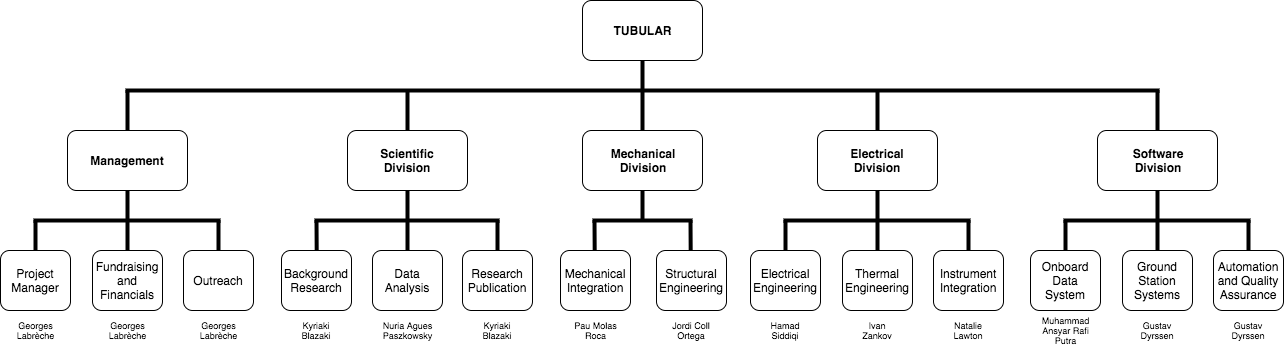
\includegraphics[width=16cm]{3-project-planning/img/work-breakdown-structure.png}
    \end{align*}
    \caption{Work Breakdown Structure}\label{fig:work-breakdown-structure}
\end{figure}

The interaction between the subteams will be refined over the course of project implementation to acknowledge the interdisciplinary nature of the experiment around a Payload / Platform scheme.

The Management is composed of a Project Manager acting as the Systems Engineer and managing overall implementation of the project. The Project Manager is responsible for establishing and overseeing product development cycle; coordinating between different teams, project stakeholders, and documentation efforts; outreach and public relations; Fundraising; monitoring and reporting; system integration; and quality assurance.

The Scientific Division is responsible for defining experiment parameters; data analysis; interpreting and documenting measurements; researching previous AirCore experiments for comparative analysis purposes; evaluating the reliability of the proposed AAC sampling system; conducting measurements of collected samples; documenting and publishing findings; defining experiment parameters; contacting researchers or institutions working on similar projects; exploring potential partnership with researchers and institutions; documenting and publishing findings.

The Mechanical Division is responsible for designing or redesigning cost-effective mechanical devices using analysis and computer-aided design; producing details of specifications and outline designs; overseeing the manufacturing process for the devices; identifying material and component suppliers; developing and testing prototypes of designed devices; analyzing test results and changing the design as needed; and integrating and assembling final design.

The Electrical Division is responsible for designing and implementing cost-effective circuitry using analysis and computer-aided design; producing details of specifications and outline designs; developing, testing, and evaluating theoretical designs; identifying material as well as component suppliers; reviewing and testing proposed designs; recommending modifications following prototype test results; and assembling designed circuitry.

The Software Division is responsible for gathering software requirements; formalizing software specifications; drafting architecture design; leading software implementation efforts; leading quality assurance and testing efforts; enforcing software testing best practices such as continuous integration testing and regression testing; reviewing requirements and specifications in order to foresee potential issues; providing input for functional requirements; advising on design; formalizing test cases; tracking defects and ensuring their resolution; facilitating code review sessions; and supporting software implementation efforts.
\pagebreak
\subsection{Schedule}

Scheduling of the project is presented in a Gantt Chart overview on Figure \ref{fig:schedule-gantt-chart}. Exam period constraints have been included in order to evaluate risks in person-day allocations to project implementation:

\begin{figure}[H]
    \begin{align*}
        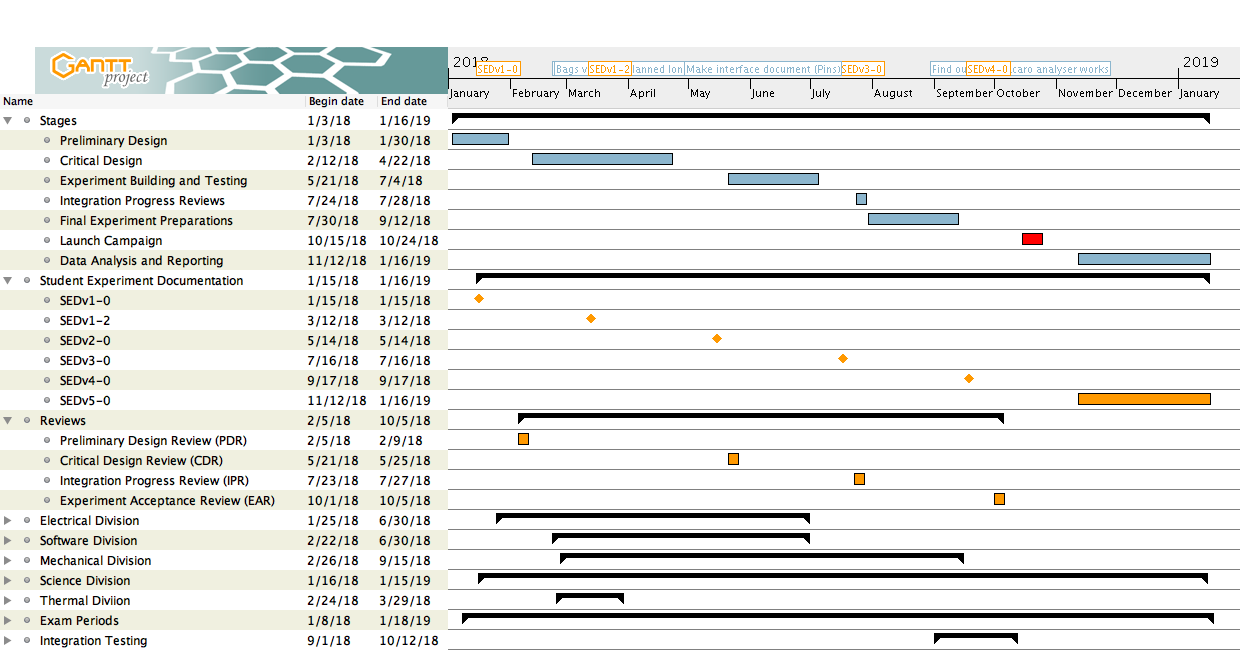
\includegraphics[width=1\linewidth]{3-project-planning/img/gantt-chart.png}
    \end{align*}
    \caption{Project Schedule Gantt Chart}\label{fig:schedule-gantt-chart}
\end{figure}

Deadlines of the five Student Experiment Documentations (SED) versions have been estimated based on past REXUS/BEXUS Cycles. A complete Gantt Chart listing tasks for each division \DIFdelbegin \DIFdel{has been included }\DIFdelend \DIFaddbegin \DIFadd{is shown }\DIFaddend in Appendix \ref{sec:appF}.
\pagebreak
\subsection{Resources}

\subsubsection{Manpower}
The TUBULAR team is categorized into divisions as summarized in Table \ref{tab:divisions-members}:

\begin{table}[H]
\centering
\resizebox{\textwidth}{!}{%
\begin{tabular}{|l|l|l|l|l|l|}
\hline
\textbf{Management} & \textbf{Scientific}    & \textbf{Mechanical} & \textbf{Electrical} & \textbf{Thermal} & \textbf{Software}          \\ \hline
Georges Labrèche*    & Kyriaki Blazaki*        & Pau Molas Roca*      & Hamad Siddiqi*  & Ivan Zankov     & Muhammad Ansyar Rafi Putra* \\ \hline
                    & Nuria Agues Paszkowsky & Jordi Coll Ortega   & Natalie Lawton  &   & Gustav Dyrssen             \\ \hline
\end{tabular}%
}
\caption{Project Divisions and Members (Asterisks Denote Division Leaders)}
\label{tab:divisions-members}
\end{table}
\raggedbottom

The experience of TUBULAR team members are listed in Table \ref{tab:team-member-experience}:

% Please add the following required packages to your document preamble:
% \usepackage{graphicx}
\begin{table}[H]
\centering
\begin{tabular}{|l|m{11cm}|}
\hline
\textbf{Team Member} & \textbf{Project Related Experience} \\ \hline
Georges Labrèche & BSc in Software Engineering with experience in technical leadership and project management in software development.\\ \hline
Nuria Agues Paszkowsky & BSc in Aerospace Engineering.\\ \hline
Kyriaki Blazaki & BSc in Physics. \\ \hline
Jordi Coll Ortega &  BSc in Aerospace Vehicle Engineering. \\ \hline
Gustav Dyrssen &  MSc in Space Engineering (4th Year).\\ \hline
Natalie Lawton & MEng in Aerospace Engineering. Previous experience in UAV avionic systems and emissions measurement techniques. \\ \hline
Muhammad Ansyar Rafi Putra & BSc in Aerospace Engineering. \\ \hline
Pau Molas Roca & BSc in Aerospace Technology Engineering, Mechanical experience. \\ \hline
Hamad Siddiqi & BSc in Electrical Engineering with experience in telecommunication industry and electronics.  \\ \hline
Ivan Zankov & BEng in Mechanical Engineering.\\ \hline
\end{tabular}
\caption{Project Related Experience of Team Members}
\label{tab:team-member-experience}
\end{table}
\raggedbottom

The initial projected effort to be contributed by each team member is of an average of 1.5 hour per person per day corresponding to a team total of 15 hours per day. Taking into account all team members, the efforts projected to be allocated to each stages of the project is summarized in Table \ref{tab:effort-allocation-stages}:

\begin{table}[H]
\centering
\begin{tabular}{l|l|l|}
\hline
\multicolumn{1}{|l|}{\textbf{Stage}} & \textbf{Duration (days)} & \textbf{Effort (hours)} \\ \hline
\multicolumn{1}{|l|}{Preliminary Design} & 28 & 420 \\ \hline
\multicolumn{1}{|l|}{Critical Design} & 70 & 1050 \\ \hline
\multicolumn{1}{|l|}{Experiment Building and Testing} & 45 & 675 \\ \hline
\multicolumn{1}{|l|}{Final Experiment Preparations} & 45 & 675 \\ \hline
\multicolumn{1}{|l|}{Launch Campaign} & 10 & 150 \\ \hline
\multicolumn{1}{|l|}{Data Analysis and Reporting} & 66 & 990 \\ \hline
\multicolumn{1}{r|}{\textbf{Total:}} & \textbf{264} & \textbf{3960} \\ \cline{2-3} 
\end{tabular}
\caption{Project Effort Allocation per Project Stages}
\label{tab:effort-allocation-stages}
\end{table}
\raggedbottom

All TUBULAR team members are based in Kiruna, Sweden, just 40 kilometers from Esrange Space Center. Furthermore, all team members are enrolled in LTU Master programmes in Kiruna and thus expected to remain in Kiruna during the entire project period. Special attention will have to be made for planning during the summer period where many team members are expected to travel abroad. An initial timeline of team member availability  until January 2019 is available in Appendix \ref{sec:appD}. A significant risk can be observed during the summer months from June to August where most members will only be partially and some completely unavailable. Team member availability and work commitments over the summer still need to be negotiated and finalized across team members in order to reduce incurred risks to the project. Furthermore, the Project Manager role will have to be assigned to another team member due to extended unavailability and partial availability.

As part of their respective Master programmes, all TUBULAR team members are enrolled in a project course at LTU. The TUBULAR project acts as the course's project for all team members from which they will obtain ECTS credits. This course is supervised by Dr. Thomas Kuhn, Associate Professor at LTU.

\pagebreak
\subsubsection{Budget}
LTU will provide financial assistance for part of the hardware expenses, approximately 250 EUR per team member\DIFdelbegin \DIFdel{, with possibility for ECTS credits}\DIFdelend . This brings the total budget to 2 500 EUR thus far. However, the total cost of the project is 8 \DIFdelbegin \DIFdel{295.04 }\DIFdelend \DIFaddbegin \DIFadd{376.65 }\DIFaddend EUR\footnote{The cost of some items have been estimated due to lack of direct quotes from vendors. A total error margin of 5\% has been included in the final budget to account for possible estimation errors.}. In order to fill this budget gap, the following potential sources of funding are to be explored throughout the first stages of the project implementation:

\begin{itemize}
    \item The Swedish National Space Board, SNSB, will be reached out to during their next open call to researchers in Sweden to apply for funding for Space Research, including Earth Observation Research.
    \item The Swedish Research Council typically opens calls for \enquote{Proof of Concept Grant – Life science} as well as \enquote{Natural and Engineering Sciences} research grants to which an application will be sent to during the upcoming 2018 calls.
    \item Meteorological institutes, research initiatives, researchers, academic institutions, and institutional donors involved in climate change will be reached out to for contributions based on the interest of collaborating in the experiment.
    \item Third-party providers of required equipment, components, and materials will be approached with an opportunity for these providers to sponsor the project through donation before considering the related expenses. Visibility of the experiment through the planned outreach programs will serve as a visibility incentive to encourage such contributions.
    \item A small online crowdfunding campaign will be organized that will primarily target contributions from the team members' first and second degree contacts.
\end{itemize}

The project budget is detailed in Table \ref{tab:budget-table}. The budget table does not include costs related to component redundancy and as such consist of the minimum cost to build the experiment. Not included in the total are components supplied by partners and potential sponsors (e.g. the CAC tube supplied by FMI). Funding from LTU covers \DIFdelbegin \DIFdel{30.01}\DIFdelend \DIFaddbegin \DIFadd{28}\DIFaddend \% of the total costs while it is projected that a SNSB grant will cover \DIFdelbegin \DIFdel{33.54}\DIFdelend \DIFaddbegin \DIFadd{31}\DIFaddend \%. The remaining costs are associated with the air sampling bags for which sponsorship will actively be sought from a manufacturer \DIFaddbegin \DIFadd{(at the time of writing, discussions with the manufacturer Restek Corporation are ongoing regarding sponsorship of air sampling bags)}\DIFaddend . 

\pagebreak
%\begin{longtable}[]
{|c|l|l|}
\hline
\multicolumn{2}{|l|}{\textbf{Expenses and Revenue per Department}} & Amount (\EUR{}) \\ \hline
\multicolumn{1}{|c|}{\multirow{5}{*}{\textbf{Electronics}}} & Components\footnote{Total cost for components is based upon Table \ref{tab:electrical-components}.} (excluding valves) & 450 \\
\multicolumn{1}{|c|}{} & Valves & 2000 \\
\multicolumn{1}{|c|}{} & Shipping Costs & 100 \\
\multicolumn{1}{|c|}{} & Tools and Equipment & 200 \\ \cline{2-3} 
\multicolumn{1}{|c|}{} & \textbf{Total Electronics Cost} & 2750 \\ \hline
\multicolumn{1}{|c|}{\multirow{6}{*}{\textbf{Mechanics}}} & Components\footnote{Total cost for mechanics is based upon Table \ref{tab:mechanical-components}.} & 450 \\
\multicolumn{1}{|c|}{} & Manufacturing & TBD \\
\multicolumn{1}{|c|}{} & Testing (Structural and Thermal) & TBD \\
%\multicolumn{1}{|c|}{} & Shipping Costs & TBD \\
\cline{2-3} 
\multicolumn{1}{|c|}{} & \textbf{Total Mechanics Cost} & TBD \\ \hline
\multicolumn{1}{|c|}{} & Project Visibility (badges, merch, website, publications, etc) & 250\\
\cline{2-3} 
\multicolumn{1}{|c|}{} & \textbf{Total Outreach} & TBD \\ \hline
\multicolumn{1}{l|}{} & \textbf{Total Costs} & TBD \\ \cline{2-3} 
\caption{Preliminary Budget Table}
\label{tab:budget-table}
\end{longtable}
\raggedbottom

\begin{table}[H]
    \begin{align*}
        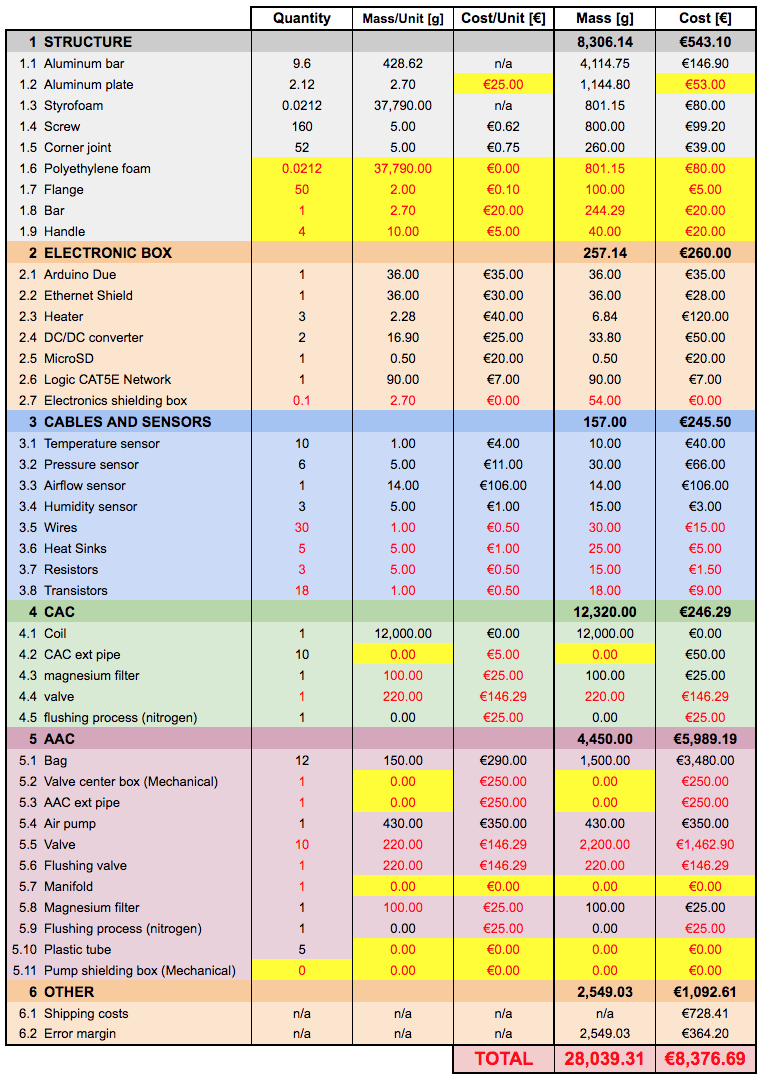
\includegraphics{3-project-planning/tables/budget-table.png}
    \end{align*}
    \caption{Project budget table. Values highlighted in yellow have yet to be determined/estimated. Number values in red have been estimated rather than determined by vendor quotes. \DIFaddbeginFL \DIFaddFL{Shipping cost is estimated at 10\% of total cost. Total cost error margin is set to 5\% of projected total cost. Total mass error margin is set to 10\% of projected total mass.}\DIFaddendFL }\label{tab:budget-table}
\end{table}


\subsubsection{External Support}

Partnership with the Finnish Meteorological Institute (FMI), and the Swedish Institute of Space Physics (IRF) will provide the team with technical guidance in implementing the sampling system. FMI’s experience in implementing past AirCore sample systems provide invaluable lessons learned towards conceptualizing, designing, and implementing the proposed AAC sampling system.

FMI is a key partner in the TUBULAR project, its scientific experts will advise and support the TUBULAR project by sharing knowledge, experience, and granting accessibility of equipment. \DIFaddbegin \DIFadd{As per the agreement shown in Appendix \ref{sec:appG}, }\DIFaddend FMI will provide the TUBULAR team with the AirCore stainless tube component of CAC subsystem as well as the post-flight gas analyzer. This arrangement requires careful considerations on the placement of the experiment in order to minimize hardware damage risks. These contributions will result in significant cost savings regarding equipment and component procurement.

Daily access to LTU's Space Campus in Kiruna will expose the team to scientific mentorship and expert guidance from both professors and researchers involved in the study of greenhouse gases and climate change. Dr Uwe Raffalski, Swedish institute of Space physics (IRF), Associate professor (Docent) is one of many researchers involved in climate study who is mentoring the team.
\pagebreak

\subsection{Outreach Approach}

The experiment as well as the BEXUS programme and its partners will be promoted through the following activities:

\begin{itemize}
\item Research paper published in partnership with the Finnish Meteorological Institute (FMI) detailing the sampling methodology, measurement result, analysis, and findings.
\item Collected data will be licensed as open data to be freely available to everyone to use and republish as they wish, without restrictions from copyright, patents or other mechanisms of control.
\item A website will be launched that will summarize the experiment and provide regular updates. Backend web analytics included to gauge interest on the project through number of visitors and their origins.
\item Dedicated Facebook page used as publicly accessible logbook detailing challenges, progress, and status of the project. Open for comments and questions (See Figure \ref{fig:outreach-facebook} in Appendix \ref{sec:appE}).
\item Two Instagram accounts for short and frequent image and video focused updates. A primary Instagram account will be dedicated to project updates. A secondary account will reach out to a broader audience by focusing on space instruments in general and cross-reference TUBULAR related activities when relevant (See Figures \ref{fig:outreach-instagram}, \ref{fig:outreach-instagram-si-1}, and \ref{fig:outreach-instagram-si-2} in Appendix \ref{sec:appE}).
\item GitHub account to host all project software code under free and open source license (See Figures \ref{fig:outreach-github} in Appendix \ref{sec:appE}). Other REXUS/BEXUS teams will be invited to host their code in this account in what will hopefully become a centralized GitHub account and code archive for present and future REXUS/BEXUS projects.
\item Reddit Ask Me Anything (AMA) thread to discuss the project with community of online enthusiasts.
\item\enquote{Show and Tell} trips to local high schools and universities. Team members will be responsible to organize such presentations through any of their travel opportunities abroad.
\item In-booth presentation and poster display in the seminars or career events at different universities. 
\item A thoroughly documented and user-friendly manual on how to build replicate and launch CAC and AAC sampling systems will be produced and published.
\end{itemize}
\pagebreak
\subsection{Risk Register}
\textbf{Risk ID}
\begin{enumerate}[label={}]
    \item TC – technical/implementation 
    \item MS – mission (operational performance) 
    \item SF – safety 
    \item VE – vehicle 
    \item PE – personnel 
    \item EN – environmental 
    \item OR - Outreach
    \item BG - Budget
\end{enumerate}

Adapt these to the experiment and add other categories. 
Consider risks to the experiment, to the vehicle and to personnel. 

\textbf{Probability (P)}
\begin{enumerate}[label=\Alph*]
    \item Minimum – Almost impossible to occur 
    \item Low – Small chance to occur 
    \item Medium – Reasonable chance to occur 
    \item High – Quite likely to occur 
    \item Maximum – Certain to occur, maybe more than once
\end{enumerate}

\textbf{Severity (S)}
\begin{enumerate}
    \item Negligible – Minimal or no impact 
    \item Significant – Leads to reduced experiment performance 
    \item Major – Leads to failure of subsystem or loss of flight data 
    \item Critical – Leads to experiment failure or creates minor health hazards 
    \item Catastrophic – Leads to termination of the BEXUS programme, damage to the vehicle or injury to personnel 
\end{enumerate}

The rankings for probability (P) and severity (S) are combined to assess the overall risk classification, ranging from very low to very high and being coloured green, yellow, orange or red according to the SED guidelines.

\begin{landscape}
\begin{longtable}{|m{0.09\textwidth}| m{0.51\textwidth} |m{0.03\textwidth} |m{0.03\textwidth}|m{0.11\textwidth}| m{0.65\textwidth}|}

\hline
\textbf{ID} & \textbf{Risk (\& consequence if)} & \textbf{P} & \textbf{S} & \textbf{P * S} & \textbf{Action} \\ \hline
TC10 & Software fails to store data & B & 4 & \cellcolor[HTML]{FCFF2F}Low & Acceptable Risk: Extensive testing will be done \\ \hline
TC20 & Failure of several sensors & B & 3 & \cellcolor[HTML]{FCFF2F}Low & \DIFaddbegin \DIFadd{Acceptable Risk: }\DIFaddend Thermal test to approve the functionality of the experiment. \\ \hline
TC30 & Critical component is destroyed in testing & B & 1 & \cellcolor[HTML]{FCFF2F}Low & Acceptable risk: Spare components can be ordered but for expensive ones, they will be ordered and tested early in the project in case we need to order more. \\ \hline
TC40 & Electrical connections dislodges or short circuits because of vibration or shock & B & 3 & \cellcolor[HTML]{FCFF2F}Low & Unacceptable risk. Careful soldering and extensive testing will be applied. \\ \hline
TC50 & Experiment electronics fail due to long exposure to cold or warm temperatures & B & 3 & \cellcolor[HTML]{FCFF2F}Low & \DIFaddbegin \DIFadd{Unacceptable Risk: }\DIFaddend Thermomechanical and thermoelectrical solutions will be simulated and tested in detail to help prevent this from happening. \\ \hline
TC60 & Software and electrical fail to control heaters causing temperature to drop or rise below or above operational range & B & 2 & \cellcolor[HTML]{34FF34}Very Low & Unacceptable risk: Tests will be performed prior to the flight to detect and minimize the risk of occurrence.The system will be monitored during flight and handled manually if necessary. \\ \hline
TC70 & Software fails to enter safe mode (may result in loss of data) & B & 3 & \cellcolor[HTML]{FCFF2F}Low & Acceptable Risk: Extensive testing will be done. \\ \hline
TC80 & On-board memory will be full (flight time longer than expected) & A & 2 & \cellcolor[HTML]{34FF34}Very Low & Acceptable Risk: The experiment shall go through testing and analysis to guarantee the onboard memory size is sufficient.\\ \hline
TC90 & Connection loss with ground station & A & 4 & \cellcolor[HTML]{34FF34}Very Low & Acceptable Risk: Experiment will be designed to operate autonomously. \\ \hline
TC100 & Software fails to control valves autonomously & B & 4 & \cellcolor[HTML]{FCFF2F}Low & Acceptable Risk: Extensive testing will be done. Telecommand will also be used to manually control the valves. \\ \hline
TC110 & Software fails to change modes autonomously & B & 4 & \cellcolor[HTML]{FCFF2F}Low & Acceptable Risk: Extensive testing will be done. Telecommand will also be used to manually change experiment modes. \\ \hline
TC120 & Complete software failure & B & 4 & \cellcolor[HTML]{FCFF2F}Low & Acceptable Risk: Watchdog timer will be applied to reset software if it freezes. \\ \hline
TC130 & Failure of fast opening system & B & 2 & \cellcolor[HTML]{34FF34}Very Low & Acceptable risk: the box could also be opened but a little bit slower. \\ \hline
TC140 & The gas analyzer isn't properly calibrated and returns inaccurate results & B & 4 & \cellcolor[HTML]{FCFF2F}Low & Acceptable risk: Calibrate the gas analyzer before use.\\ \hline
MS10 & Down link connection is lost prematurely & B & 2 & \cellcolor[HTML]{34FF34}Very Low & Acceptable Risk: Data will also be saved on SD card. \\ \hline
MS20 & Condensation on experiment PCBs which could causes short circuits & A & 3 & \cellcolor[HTML]{34FF34}Very Low & Acceptable risk: Circuit box will be sealed to prevent condensation. \\ \hline
MS30 & Temperature sensitive components that are essential to full the mission objective might be below their operating temperature. & C & 3 & \cellcolor[HTML]{FCFF2F}Low & \DIFaddbegin \DIFadd{Acceptable Risk: }\DIFaddend Safe mode to prevent the components to operate out of its operating temperature range. \\ \hline
MS40 & Experiment lands in water causing electronics failure & B & 1 & \cellcolor[HTML]{34FF34}Very Low & Acceptable risk: Check if SD card needs waterproof shell or is waterproof in itself. Also, all the necessary data will be downloaded during the flight. \\ \hline
MS50 & Interference from other experiments and/or balloon & A & 4 & \cellcolor[HTML]{34FF34}Very Low & Acceptable risk: no action. \\ \hline
MS60 & Balloon power failure & C & 1 & \cellcolor[HTML]{34FF34}Very Low & Acceptable risk: Valves default state is closed so if all power is lost valves will automatically close preserving all samples collected up until that point. \\ \hline
MS70 & Bags disconnect & C & 3 & \cellcolor[HTML]{FCFF2F}Low & \DIFaddbegin \DIFadd{Acceptable Risk: }\DIFaddend The affected bags could not collect samples. A proper fixing of the flanges must be double checked.
\\ \hline
\DIFdelbegin \DIFdel{MS80 }\DIFdelend \DIFaddbegin \DIFadd{MS71 }\DIFaddend & Bags puncture & B & 3 & \cellcolor[HTML]{FCFF2F}Low & \DIFaddbegin \DIFadd{Acceptable Risk: }\DIFaddend The affected bags could not collect samples. Proper protection will be placed in order to avoid puncture from external elements. \\ \hline
\DIFdelbegin \DIFdel{MS90 }\DIFdelend \DIFaddbegin \DIFadd{MS72 }\DIFaddend & \DIFaddbegin \DIFadd{Bags' hold time is typically 48h }& \DIFadd{C }& \DIFadd{3 }& \cellcolor[HTML]{FCFF2F}\DIFadd{Low }& \DIFadd{Acceptable risk: Validation studies can demonstrate longer stability.  }\\ \hline
\DIFadd{MS80 }& \DIFaddend Pump failure & C & 4 & \cellcolor[HTML]{ffae42}Medium & \DIFdelbegin \DIFdel{The bags could }\DIFdelend \DIFaddbegin \DIFadd{Unacceptable risk: The bags would }\DIFaddend not be filled and thus the AAC system would fail. The pump will be properly chosen \DIFdelbegin \DIFdel{and }\DIFdelend \DIFaddbegin \DIFadd{based on past research and extensively }\DIFaddend tested before the flight. \\ \hline
\DIFdelbegin \DIFdel{MS100 }\DIFdelend \DIFaddbegin \DIFadd{MS90 }\DIFaddend & Intake pipe blocked by external element & C & 3 & \cellcolor[HTML]{FCFF2F}Low & \DIFdelbegin \DIFdel{The bags could }\DIFdelend \DIFaddbegin \DIFadd{Unacceptable Risk: The bags would }\DIFaddend not be filled and thus the AAC system would fail. An air filter will be placed in both intake and outlet of the pipe to prevent \DIFdelbegin \DIFdel{it}\DIFdelend \DIFaddbegin \DIFadd{this}\DIFaddend . \\ \hline
VE10 & SD-card is destroyed at impact & B & 3 & \cellcolor[HTML]{FCFF2F}Low & Acceptable Risk: All data will be transmitted to the ground. \\ \hline
VE20 & Gondola Fixing Interface & B & 4 & \cellcolor[HTML]{FCFF2F}Low & \DIFaddbegin \DIFadd{Unacceptable Risk: }\DIFaddend The experiment box could detach from the gondola’s rails and the two boxes could detach one from the other. Proper fixing has been designed to prevent it. \\ \hline
VE30 & Structure damage due to bad landing & B & 3 & \cellcolor[HTML]{FCFF2F}Low & \DIFaddbegin \DIFadd{Acceptable Risk: }\DIFaddend Landing directly on a hard element could break the structure or the protective walls. Consistent design implemented to prevent it. \\ \hline
VE40 & Hard landing damages the CAC equipment & C & 3 & \cellcolor[HTML]{FCFF2F}Low & Acceptable risk:  Proper  protection will be placed in order to avoid damage from hard landing. \\ \hline
VE50 & Hard landing damages the AAC equipment & C & 3 & \cellcolor[HTML]{FCFF2F}Low & Acceptable risk:  Proper  protection will be placed in order to avoid puncture from hard landing. \\ \hline
EN10 & Vibrations & C & 1 & \cellcolor[HTML]{34FF34}Very Low & Acceptable risk: Vibrations do not affect the sampled air. \\ \hline
EN20 & The air samples must be protected from direct sunlight and \DIFdelbegin \DIFdel{store }\DIFdelend \DIFaddbegin \DIFadd{stored }\DIFaddend above 0 \degree C to prevent condensation & D & 4 & \cellcolor[HTML]{FF0800}High risk & Unacceptable risk\DIFaddbegin \DIFadd{: Further test regarding insulation performance and humidity levels in the bags will be done.  }\DIFaddend \\ \hline 
PE10 & The Project Manager is no longer available to manage the project. & E & 1 & \DIFdelbegin %DIFDELCMD < \cellcolor[HTML]{FF0800}%%%
\DIFdel{High risk }\DIFdelend \DIFaddbegin \cellcolor[HTML]{FCFF2F}\DIFadd{Low }\DIFaddend & Acceptable risk: The Deputy Project Manager will take over as Project Manager. \\ \hline 
PE20 & Team members from the same division are unavailable during the same period over the summer. & C & 4 & \cellcolor[HTML]{ffae42}Medium risk & Unacceptable risk: Summer travel schedules to be coordinated among team members and approved by Project Manager. \\ \hline 
% & & & & &\\ \hline

%\end{tabular}
\caption{Risk Register}
\label{tab:risk-register}
\end{longtable}
\raggedbottom
\end{landscape}

\pagebreak
\section{Experiment Design}
\subsection{Experiment Setup} \label{Experiment_Setup}

The experiment consists of AAC ten sampling bags subsystem, and the CAC coiled tube subsystem. The principal aim is to validate the AAC sampling method and to do so, it is necessary to sample during descent phase in order to compare the results with the ones obtained from the CAC. All speeds mentioned in this section have been obtained from the BEXUS manual as well as through analysis of past flights.

The primary concern regarding the AAC air sampling subsystem is that after cut-off the gondola will tumble and fall at an average speed of 50 m/s for approximately 2 minutes \cite{BexusManual}. This falling speed is too fast in order to sample air at the desired vertical resolution that is targeted to be 500m. This means that only after the gondola is stabilized at a descent rate of 8 m/s \cite{BexusManual} the sampling can be done. The tumbling phase will span approximately for 6km and considering a floating phase at 25km, the sampling can be started from 19km in altitude. Nevertheless, the main region of interest is the stratosphere, especially between 19km and 25km of altitude. It is for this reason that the team has decided to sample during ascent phase as well. Ten sampling bags will be filled up, six during ascent phase approximately between 18-24km, and four during descent phase below 19km. The desired vertical resolution is 500 m at a falling speed of 8 m/s which means that using bags with a volume of 3L, an air pump with at least 3L/min intake rate is necessary for the sampling bags.

\DIFdelbegin \DIFdel{It has to be taken into account the }\DIFdelend \DIFaddbegin \DIFadd{The }\DIFaddend maximum pressure that the sampling bags can withstand \DIFaddbegin \DIFadd{has to be taken into account }\DIFaddend in order to avoid bursting. During ascent phase, due to the decreasing pressure, the bags with the air samples , will expand which may have risk of bursting. To avoid this, the bags should not be fully sampled. The providers recommend not to fill more than 80 percent (~2psi/0.14bar) for Multi-Layer Foil bags. The opposite applies for descent phase. The bags with the air samples, will be compressed, and in order to assure that the samples are enough for analysis, they should be fully filled. It has to be mentioned that it has been found from past research \DIFaddbegin \DIFadd{\mbox{%DIFAUXCMD
\cite{LISA} }\hspace{0pt}%DIFAUXCMD
}\DIFaddend that the same bags can withstand a difference in pressure between outside and inside of 310hPa at 30km of altitude, which is equivalent to 0.31bar. Therefore, future test will confirm the maximum pressure for the bags.

Depending on the altitude of sampling, the range of the sample size is between 0.2L and 0.8L, with 0.2L being the minimum amount required for the chromatographer to analyse. 

The AAC will need an air pump for sampling, due to low ambient pressure at stratospheric altitudes. The air pump is also needed in order to assure the intake flow rate and obtain a good resolution. A control valve will be used to flush the pump after each bag is filled and make sure that the next bag will be filled with fresh air from the corresponding altitude. Each sampling bag will be assigned a 500 meter altitude sampling range from which to collect air samples. At an ascent speed of 5 m/s during the Ascent Phase and at a descent speed of 8 m/s during the Descent Phase. 

Shortly after the launch, the CAC valve will be opened in order to \DIFdelbegin \DIFdel{flush }\DIFdelend \DIFaddbegin \DIFadd{allow flushing }\DIFaddend the inert gas that is inside the tube, while the AAC valves will be closed until reaching the sampling altitude. Flushing of the CAC tube \DIFdelbegin \DIFdel{will be done }\DIFdelend \DIFaddbegin \DIFadd{happens }\DIFaddend passively through the progressive decrease in air pressure during the balloon's ascent phase. The CAC valve will remain open at all time during ascent, floating, and descent phases. The tube will empty itself due to pressure gradient during the ascent phase and it will be filled passively during descent. The valve will close just after hitting the ground in order to preserve the sample. The AAC will need an air pump for sampling, due to low ambient pressure. The air pump is also needed in order to assure the intake flow rate and obtain a good resolution.

After sampling for a given bag is complete, the pump will be flushed and prior to the subsequent sampling bag valve being opened. This process continues until the last sampling bag is filled.This procedure occurs twice, the first time during the Ascent Phase for the \DIFdelbegin \DIFdel{10 }\DIFdelend \DIFaddbegin \DIFadd{6 }\DIFaddend first sampling bags and the second time during the descent phase for the remaining \DIFdelbegin \DIFdel{6 }\DIFdelend \DIFaddbegin \DIFadd{4 }\DIFaddend sampling bags.

\DIFdelbegin \DIFdel{Three pressure sensors and two temperature sensors will be used. The data will be collected for both systems }\DIFdelend \DIFaddbegin \DIFadd{The ambient pressure will be measured by three pressure sensors located inside the experiment box. Only one of them is necessary for }\DIFaddend AAC and CAC\DIFdelbegin \DIFdel{. Temperature inside the bags or the AirCore will not be measured directly because it }\DIFdelend \DIFaddbegin \DIFadd{, but three sensors will be used for redundancy reasons. The pressure inside the AirCore }\DIFaddend is assumed to \DIFdelbegin \DIFdel{quickly adjust to the ambient temperature. Therefore only two sensors measuring ambient temperature will be necessary (one for CAC and another for AAC). The ambient pressure will be measured with two more sensors, one }\DIFdelend \DIFaddbegin \DIFadd{be the same as the ambient pressure, therefore no sensor is needed. To measure the pressure inside the bags, three more sensors will be allocated inside the valve center. To measure ambient temperature in the AirCore, three sensors will be allocated in the styrofoam whereas three more }\DIFaddend for the bags \DIFdelbegin \DIFdel{and one for the AirCore. For the inside pressure in the bags, one more sensor will be located insidethe manifold. To have redundancy, each of the measurements mentioned above will be made with three different sensors }\DIFdelend \DIFaddbegin \DIFadd{will be placed in the valve center. Temperature inside the bags/AirCore is assumed to quickly adjust to the ambient temperature, therefore there will not be differentiation in between inside/outside temperature. In total, there will be six pressure sensors and six temperature sensors}\DIFaddend . 


The sampling of the AAC will be triggered by the pressure \DIFdelbegin \DIFdel{read }\DIFdelend \DIFaddbegin \DIFadd{reading }\DIFaddend from the sensors \DIFaddbegin \DIFadd{inside the valve center}\DIFaddend . When the required pressure is reached, the valve will open and the sampling will start. The closing of the valve depends on two conditions and it will be triggered when either one of the conditions is true. These conditions are: maximum sampling time or maximum pressure difference between inside/outside the bags. They are determined from past research but in the future will be determined by testing. 

The emptying and sampling sequence is represented in Figures \ref{fig:ascent} and \ref{fig:descent}. It should be kept in mind that the different pressures are what triggers the opening of the valves. 

\begin{figure}[H]
    \begin{align*}
        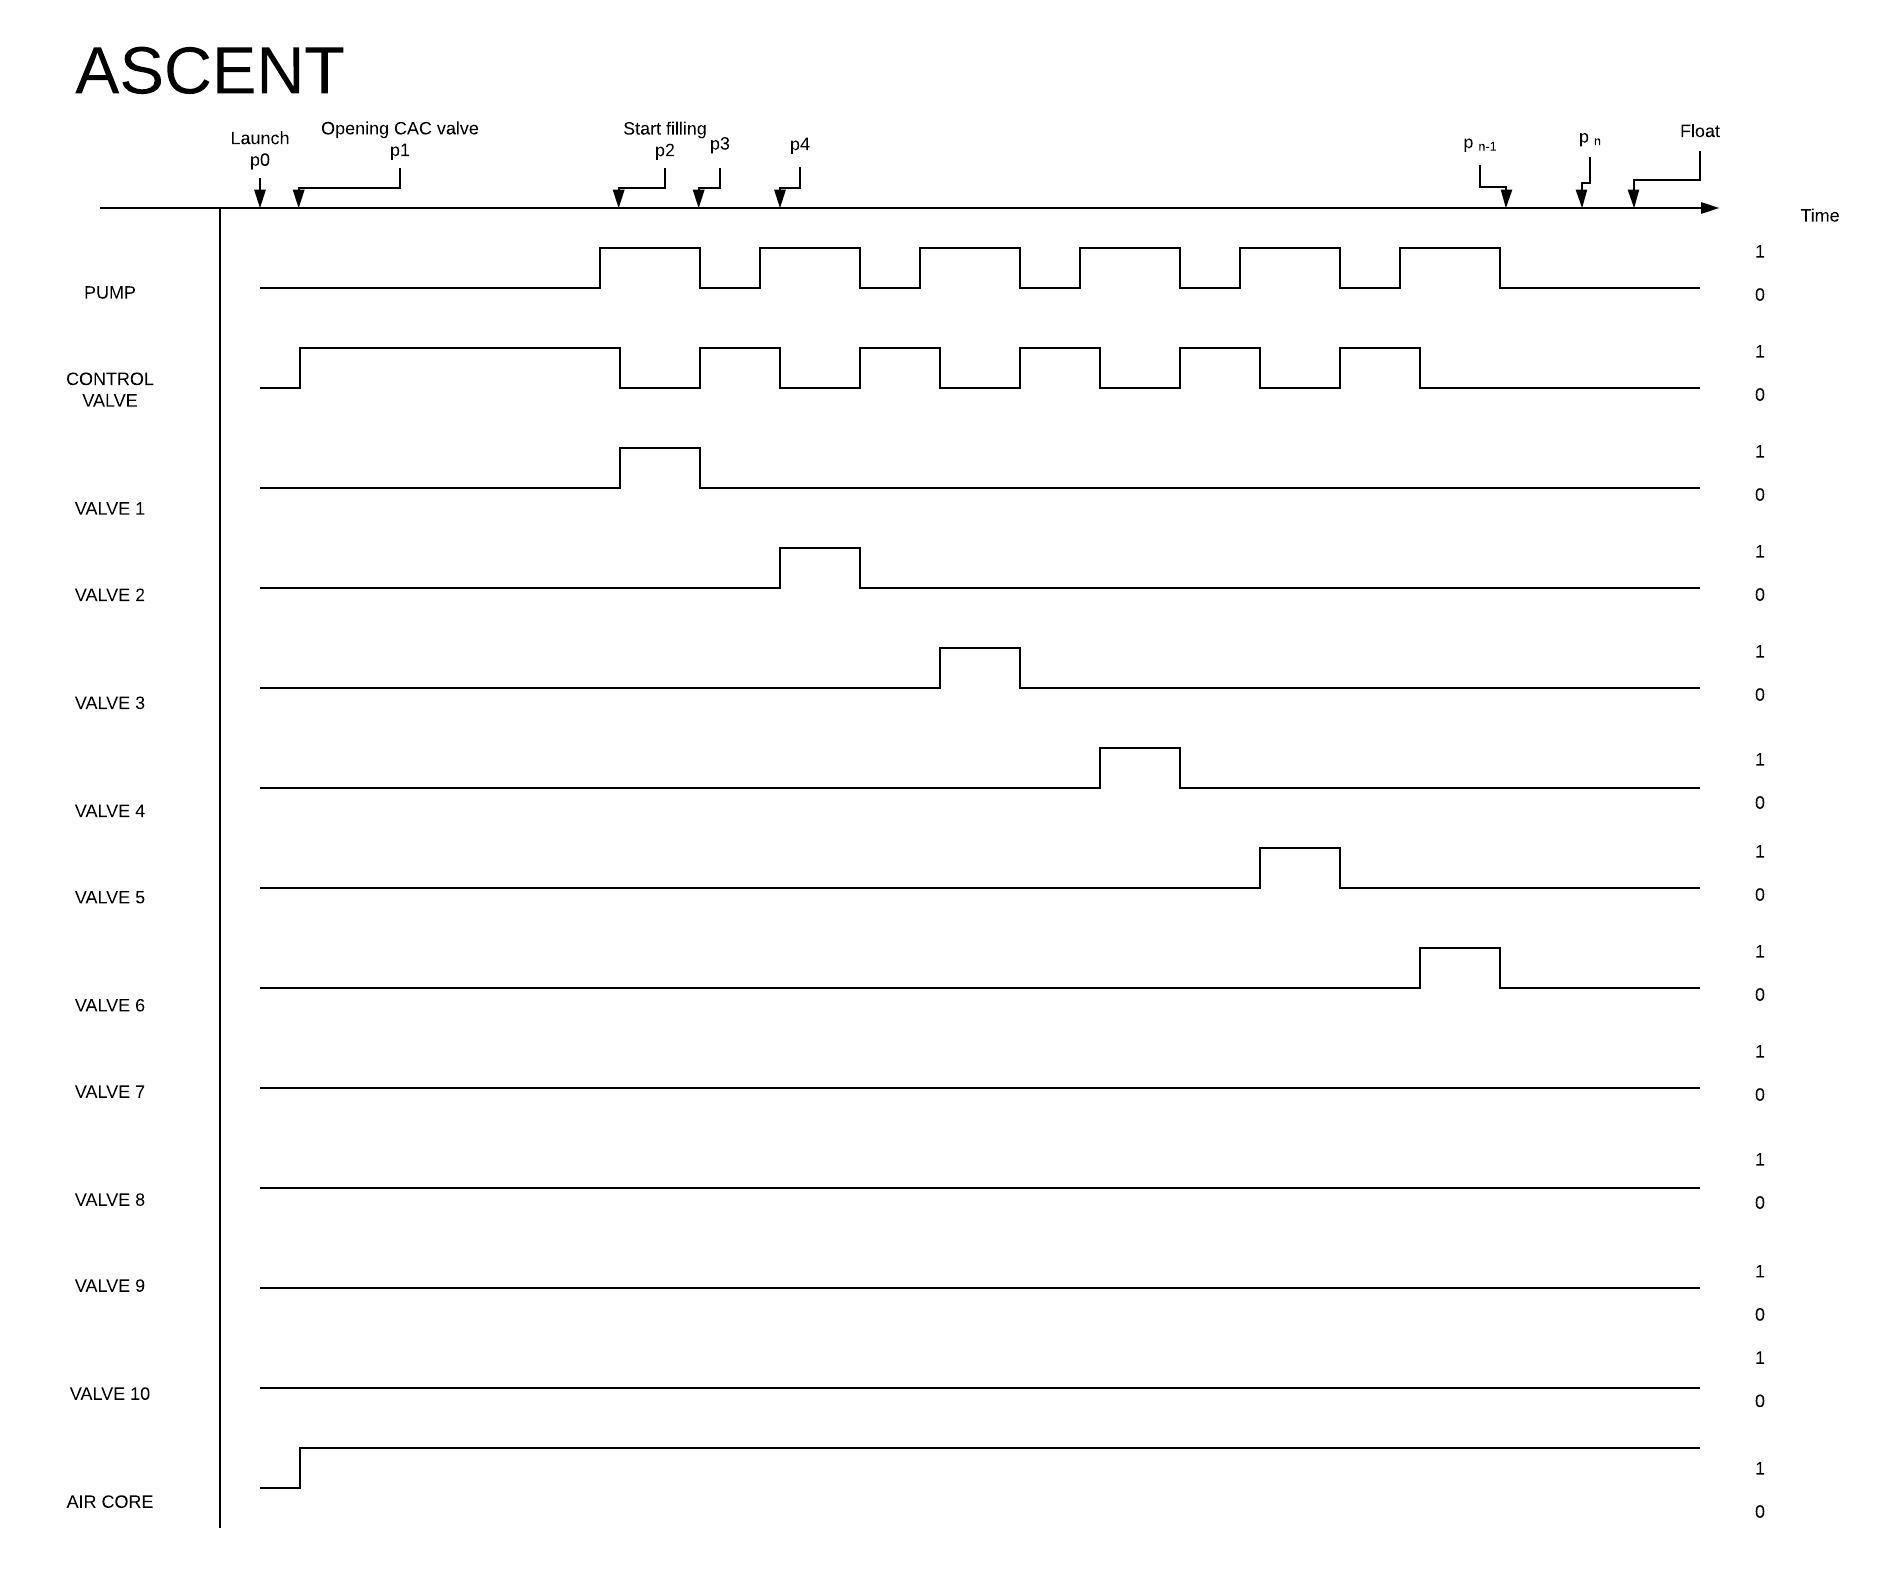
\includegraphics[width=1\linewidth]{4-experiment-design/img/ascent-phase.jpeg}
    \end{align*}
    \caption{The emptying and sampling sequence-Ascent Phase\label{fig:ascent}}
\end{figure}

\begin{figure}[H]
    \begin{align*}
        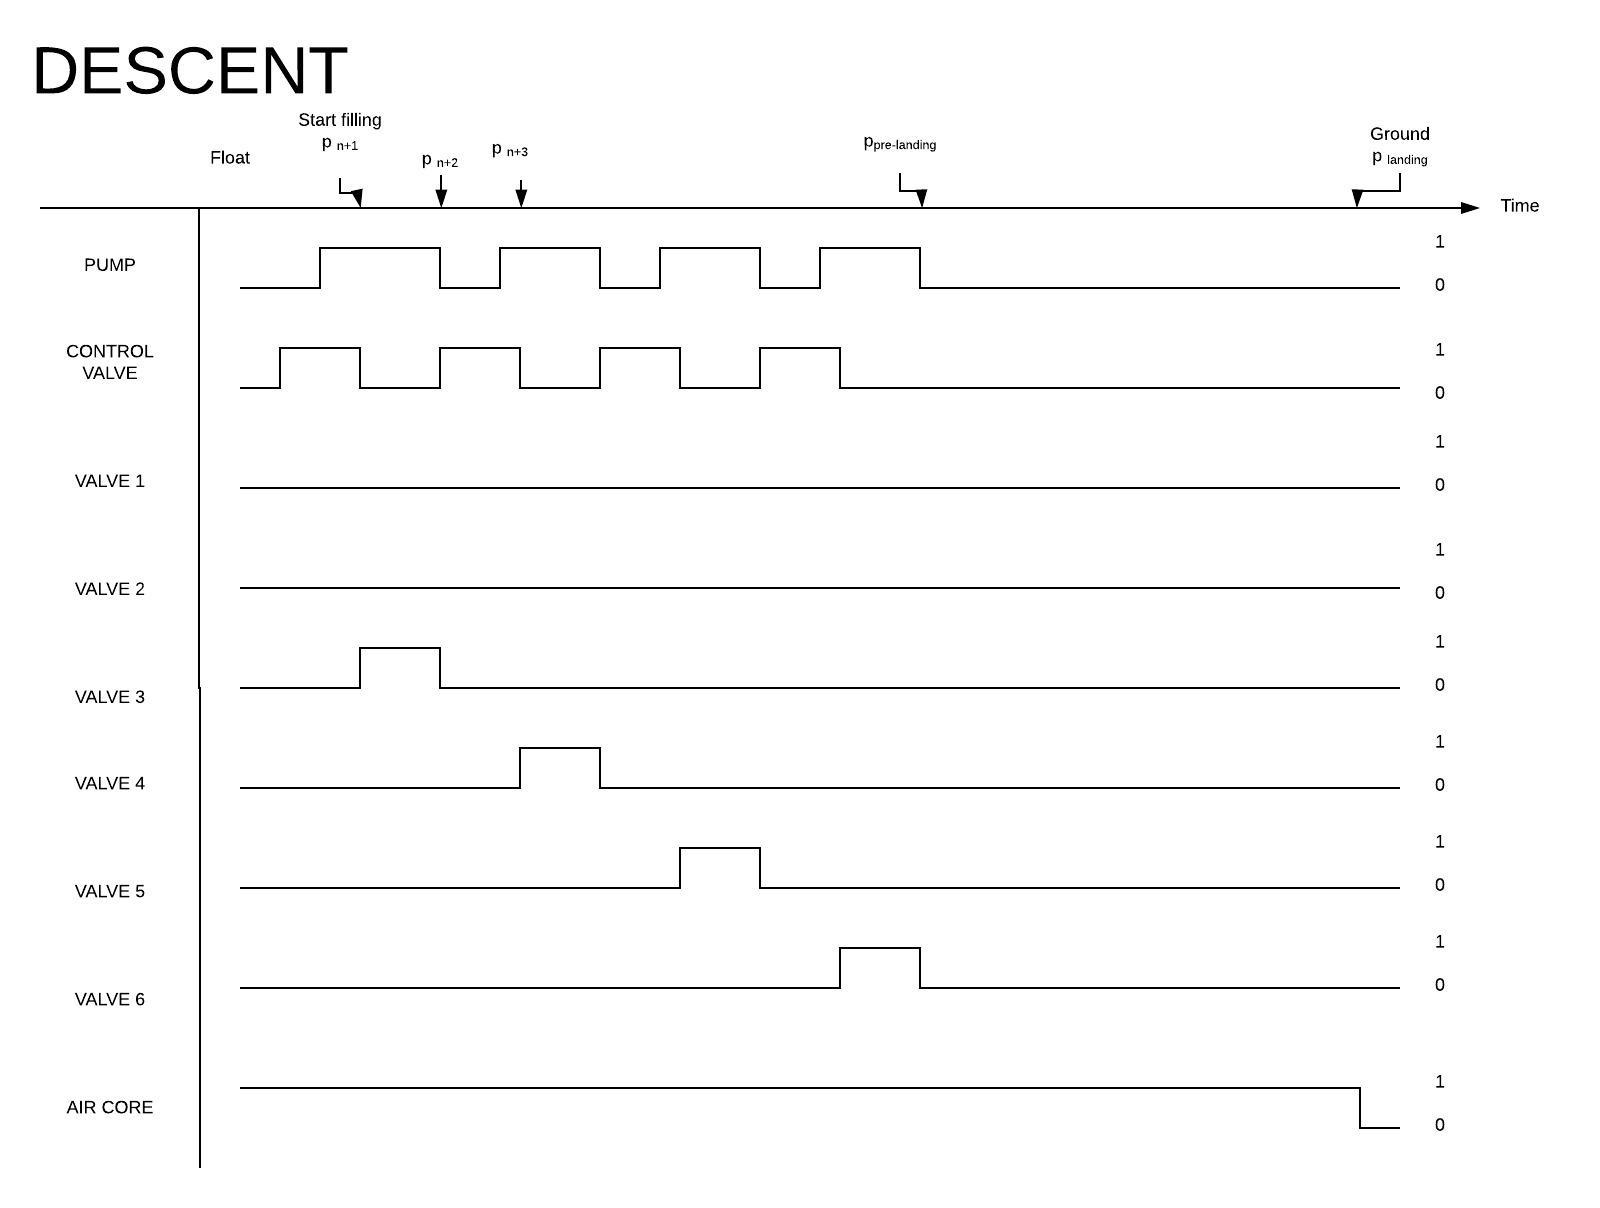
\includegraphics[width=1\linewidth]{4-experiment-design/img/descent-phase.jpeg}
    \end{align*}
    \caption{The emptying and sampling sequence-Descent Phase\label{fig:descent}}
\end{figure}

In the diagrams, 0 denotes closed/off and 1 denotes opened/on.

The general timeline of the experiment is as follow:

\textbf{Ascent Phase:}\\
$p_0$ – $p_1$
\begin{itemize}
    \item CAC valve shall be closed.
    \item AAC valves shall be closed.
    \item AAC' control valve shall be closed.
    \end{itemize}
$p_1$ – $p_2$
\begin{itemize}
    \item CAC valve shall be opened.
    \item AAC valves shall be closed.
    \item CAC tube shall be flushed.
    \item AAC' control valve shall be open.
    \end{itemize}
$p_2$ – $p_3$
\begin{itemize}
    \item Sampling bags' control valve shall be closed.
    \item Sampling bag valve 1 shall be opened, allowing for air to enter the first bag.
    \item CAC valve remains open.
    \end{itemize}
$p_3$ – $p_4$
\begin{itemize}
    \item Sampling bag valve 1 shall be closed
    \item Sampling bags' control valve shall be opened, allowing the system to flush. 
    \end{itemize}
\DIFdelbegin \DIFdel{\mbox{%DIFAUXCMD
$t_4$
}%DIFAUXCMD
}\DIFdelend \DIFaddbegin \DIFadd{\mbox{%DIFAUXCMD
$p_4$
}%DIFAUXCMD
}\DIFaddend - \DIFdelbegin \DIFdel{\mbox{%DIFAUXCMD
$t_{n-1}$
}%DIFAUXCMD
}\DIFdelend \DIFaddbegin \DIFadd{\mbox{%DIFAUXCMD
$p_{n-1}$
}%DIFAUXCMD
}\DIFaddend \begin{itemize}
    \item The above procedures shall repeat itself until the remaining \DIFdelbegin \DIFdel{nine }\DIFdelend \DIFaddbegin \DIFadd{five }\DIFaddend bags have collected air samples for their assigned altitudes.
    \end{itemize}
$p_{n-1}$ – $p_n$
\begin{itemize}
    \item Sampling bag valve \DIFdelbegin \DIFdel{10 }\DIFdelend \DIFaddbegin \DIFadd{6 }\DIFaddend shall be closed.
    \item Sampling bags' control valve shall be closed.
\end{itemize}


\textbf{\\Float Phase:}\\
No action taken other than continued telemetry. Air pump is off.\\

\textbf{Descent Phase:}

Note: Before sampling starts again, the system has to be flushed. 

$p_{n+1}$ – $p_{n+2}$
\begin{itemize}
    \item Sampling bags' control valve shall be closed.
    \item Sampling bag valve \DIFdelbegin \DIFdel{11 }\DIFdelend \DIFaddbegin \DIFadd{7 }\DIFaddend shall be opened, allowing for air to enter the first bag.
\end{itemize}

$p_{n+2}$ – $p_{n+3}$
\begin{itemize}
    \item Sampling \DIFdelbegin \DIFdel{bags' control valve }\DIFdelend \DIFaddbegin \DIFadd{bag valve 7 }\DIFaddend shall be closed
    \DIFdelbegin \DIFdel{and sampling bag valve 12 }\DIFdelend \DIFaddbegin \item \DIFadd{Sampling bags' control valve }\DIFaddend shall be opened\DIFaddbegin \DIFadd{, allowing the system to flush}\DIFaddend . 
\end{itemize}

In between, same procedure shall repeat itself until all the remaining bags have collected air samples for their assigned altitudes.

$p_{pre-landing}$ 
\begin{itemize}
    \item System \DIFdelbegin \DIFdel{shuts down:}\DIFdelend Sampling bag valve \DIFdelbegin \DIFdel{16 }\DIFdelend \DIFaddbegin \DIFadd{10 }\DIFaddend shall be closed.
    \item Sampling bags' control valve shall be closed
    \item CAC valve shall be \DIFaddbegin \DIFadd{opened.
}\end{itemize}


\DIFadd{\mbox{%DIFAUXCMD
$p_{landing}$
}%DIFAUXCMD
}\begin{itemize}
    \item \DIFadd{CAC valve shall be }\DIFaddend closed.
\end{itemize}


Note: The AAC system's air pump is only on during sampling into the air sampling bags and flushing of the system.


\raggedbottom
\pagebreak
\subsection{Experiment Interfaces}

\subsubsection{Mechanical Interfaces}
The experiment box will be fixed to the gondola rails by means of 4 screws interfacing the experiment outside structure with the hammer nuts in the rails. 90-degree aluminum angles will be used to provide this interface.This method is secure as well as fast enough to provide an accessible and easy recuperation for the later analysis. 

Lateral and top handles will be mounted to facilitate the experiment box manipulation when moving it in and out of the gondola. 

In order to collect reliable air samples, the experiment requires to be mounted at least with one side exposed to the outside. The later will reduce the pipe length used to collect clean air. Three tubes will extend from the experiment box face, see \DIFdelbegin \DIFdel{Figures \ref{fig:pipes_interface}and \ref{fig:pipes_interface_1}}\DIFdelend \DIFaddbegin \DIFadd{Figure \ref{fig:pipes_interface}}\DIFaddend . One for the CAC sampling and two, input and output, for the AAC sampling. The one-way selected method will provide a proper flushing of the pipe and thus ensure a reliable sampling as explained in section \ref{Experiment_Setup}.

\DIFaddbegin \begin{figure}[H]
    \begin{align*}
        \DIFaddFL{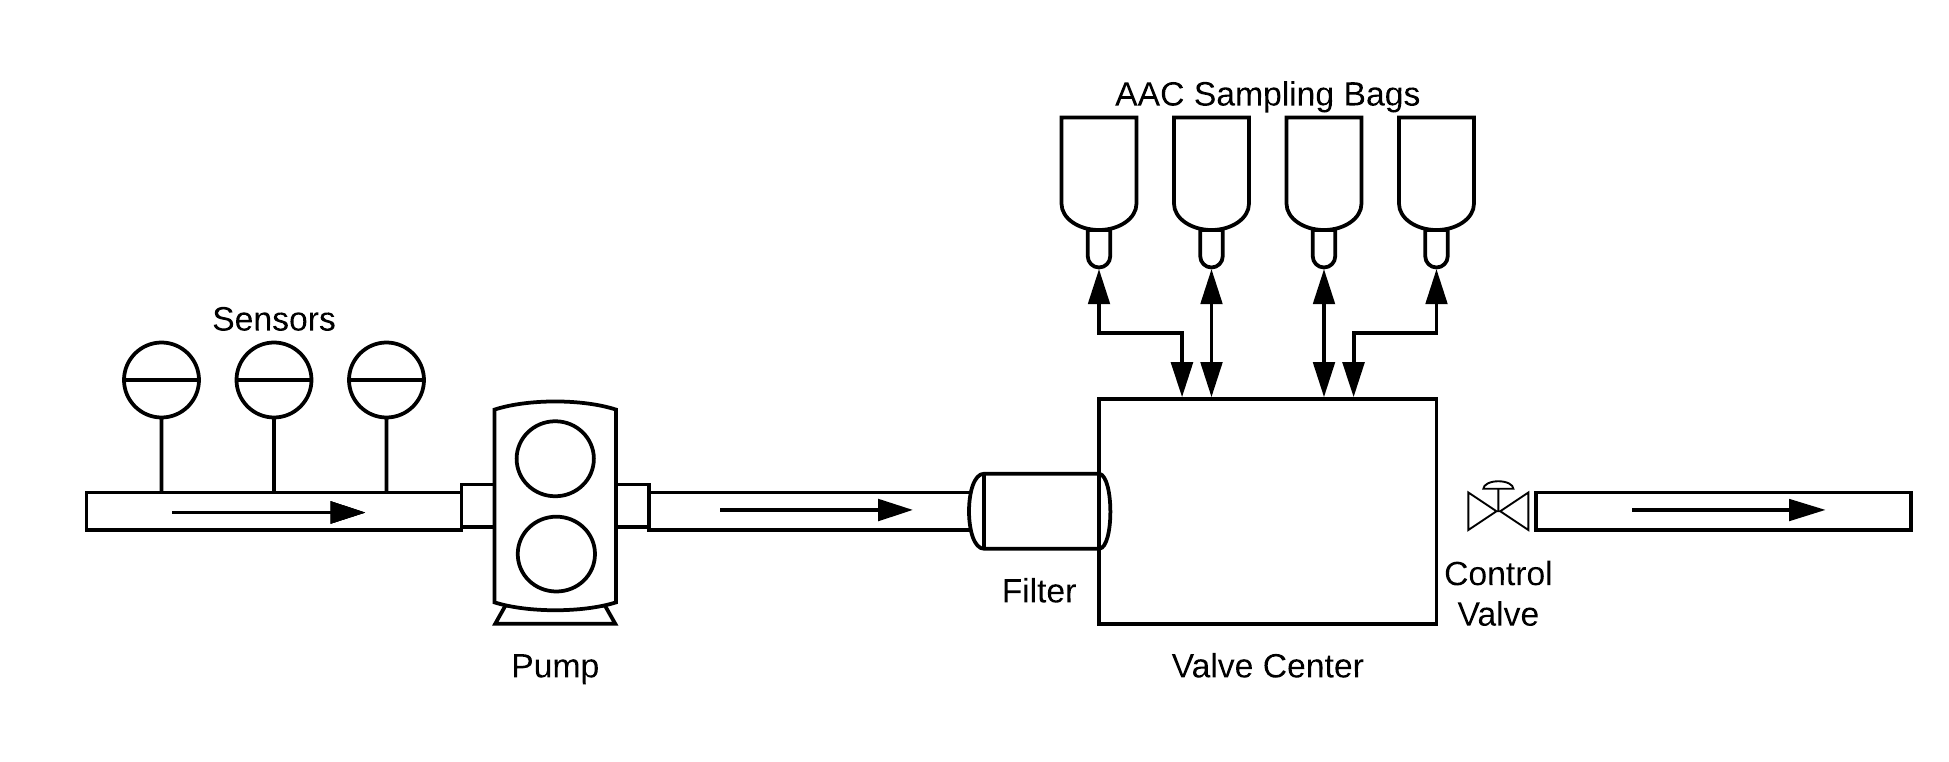
\includegraphics[width=0.7\textwidth]{4-experiment-design/img/Schematic_pipe.png}
    }\end{align*}
    \caption{\DIFaddFL{Schematic of air sampler pipe.}}\label{fig:pipes_interface}
\end{figure}

\DIFaddend \bigskip

\subsubsection{Electrical Interfaces}
\begin{centering}
The experiment will connect to the gondola electrically via a 4 pin, male, box mount receptacle MIL - C-26482P series 1 connector with an 8-4 insert arrangement (MS3112E8-4P) \cite{BexusManual}. It will connect to one 28.8V/1mA battery pack which consists of eight SAFT LSH20 batteries in series where each has a 5A fuse\cite{BexusManual}. The expected maximum current is 1.33A.
\end{centering}
\bigskip

\begin{centering}
The E-Link connection shall be made between the experiment and the E-Link system using a RJ45 connection which will be supplied by SSC and an Ethernet protocol. The Amphenol RJF21B connector will be mounted on either the front or the side of the experiment\cite{BexusManual}.  
\end{centering}
\bigskip

\begin{centering}
The expected data rate is 2kbit/s with 10kbit/s peak downlink and 5kbit/s peak uplink.
\end{centering}

\DIFdelbegin %DIFDELCMD < \begin{figure}[H]
%DIFDELCMD <     %%%
\begin{align*}
        \DIFdelFL{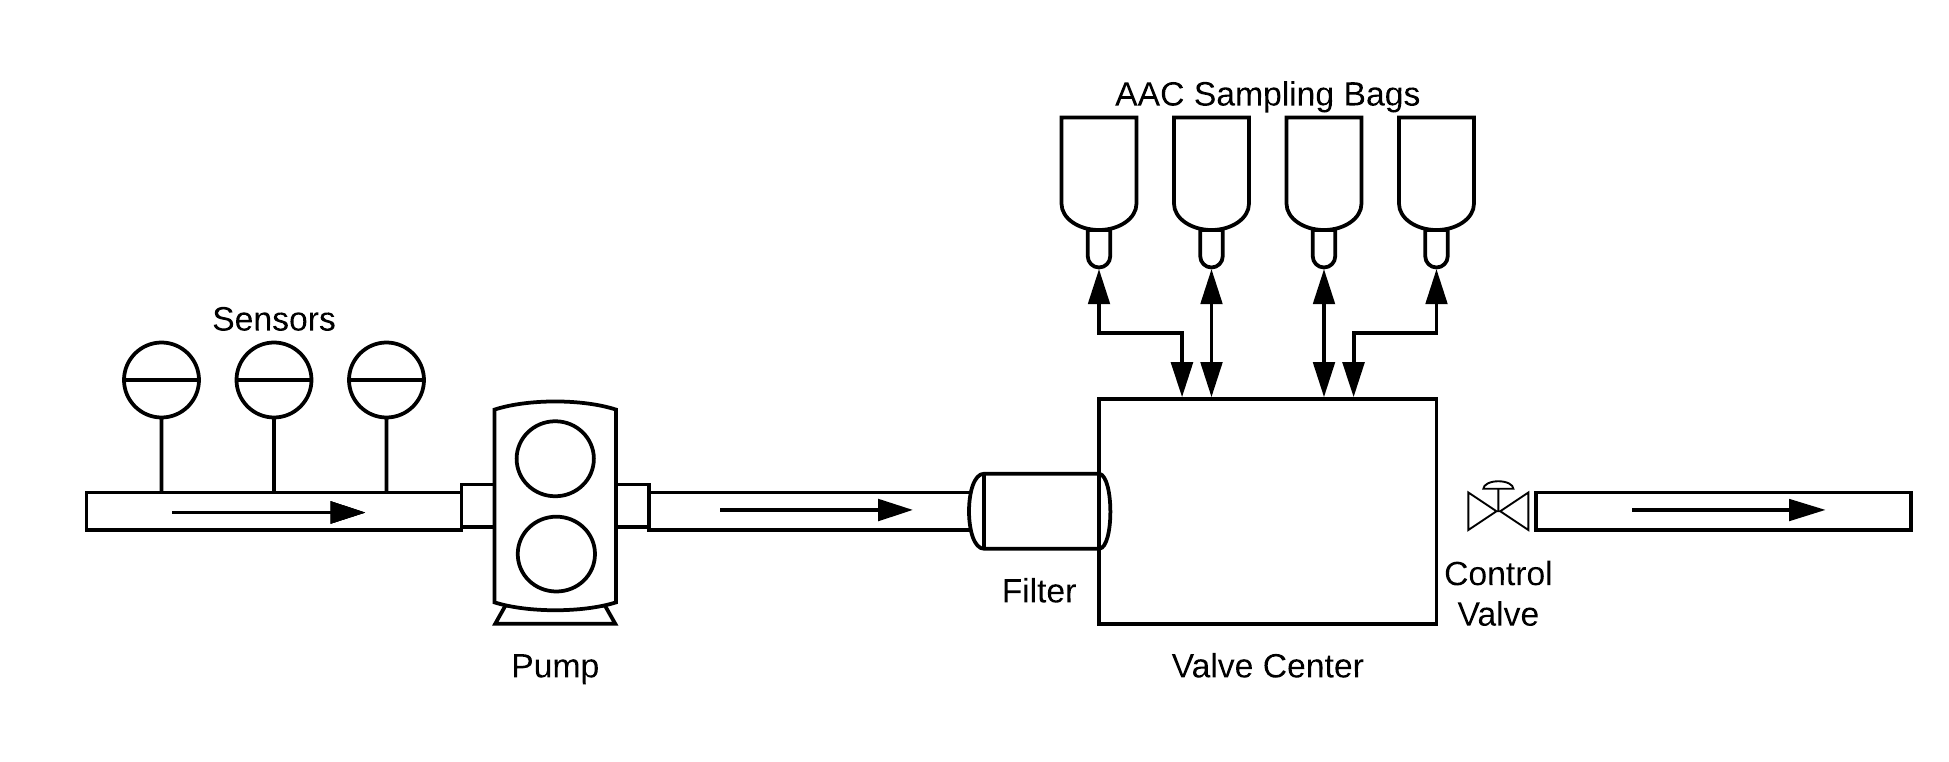
\includegraphics[width=0.7\textwidth]{4-experiment-design/img/Schematic_pipe.png}
    }\end{align*}
    %DIFAUXCMD
%DIFDELCMD < \caption{%
{%DIFAUXCMD
\DIFdelFL{Schematic of air sampler pipe.}}%DIFAUXCMD
%DIFDELCMD < \label{fig:pipes_interface}
%DIFDELCMD < \end{figure}
%DIFDELCMD < %%%
\DIFdelend %DIF > \begin{figure}[H]
%DIF >     \begin{align*}
%DIF >         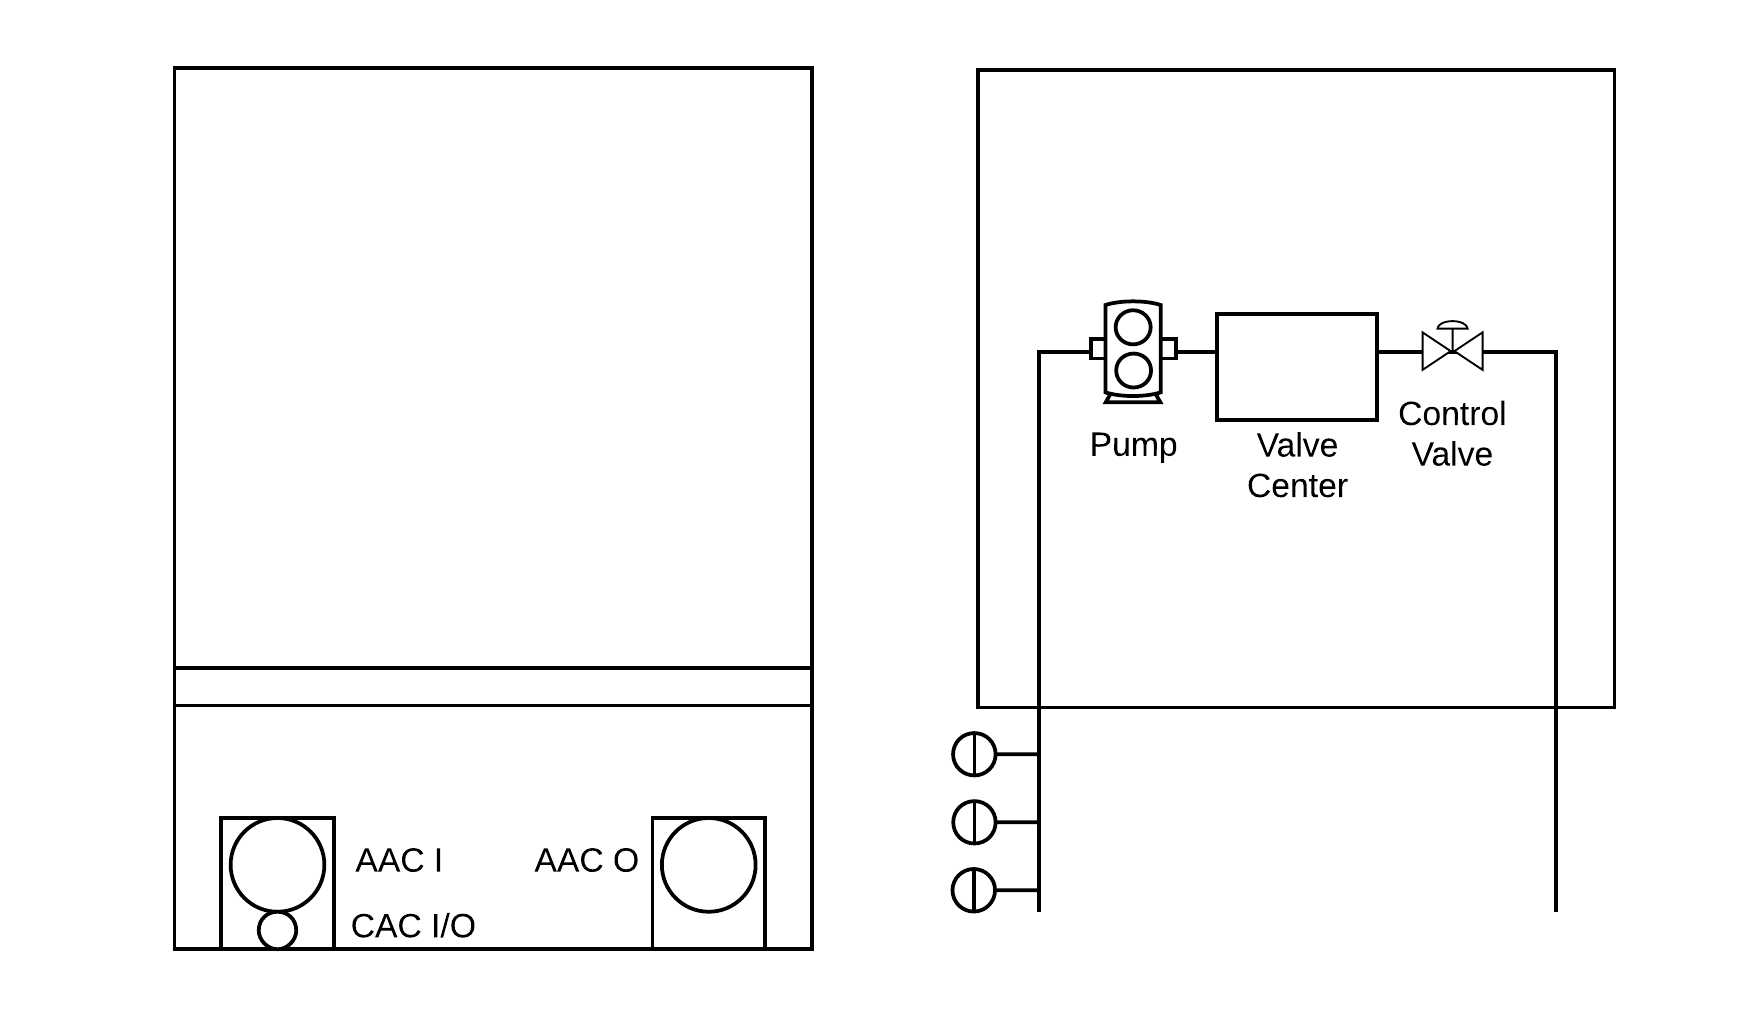
\includegraphics[width=0.7\textwidth]{4-experiment-design/img/Diagram_pipe.png}
%DIF >     \end{align*}
%DIF >     \caption{Diagram of the experiment box face exposed to the outside.}\label{fig:pipes_interface_1}
%DIF > \end{figure}

\DIFdelbegin %DIFDELCMD < \begin{figure}[H]
%DIFDELCMD <     %%%
\begin{align*}
        \DIFdelFL{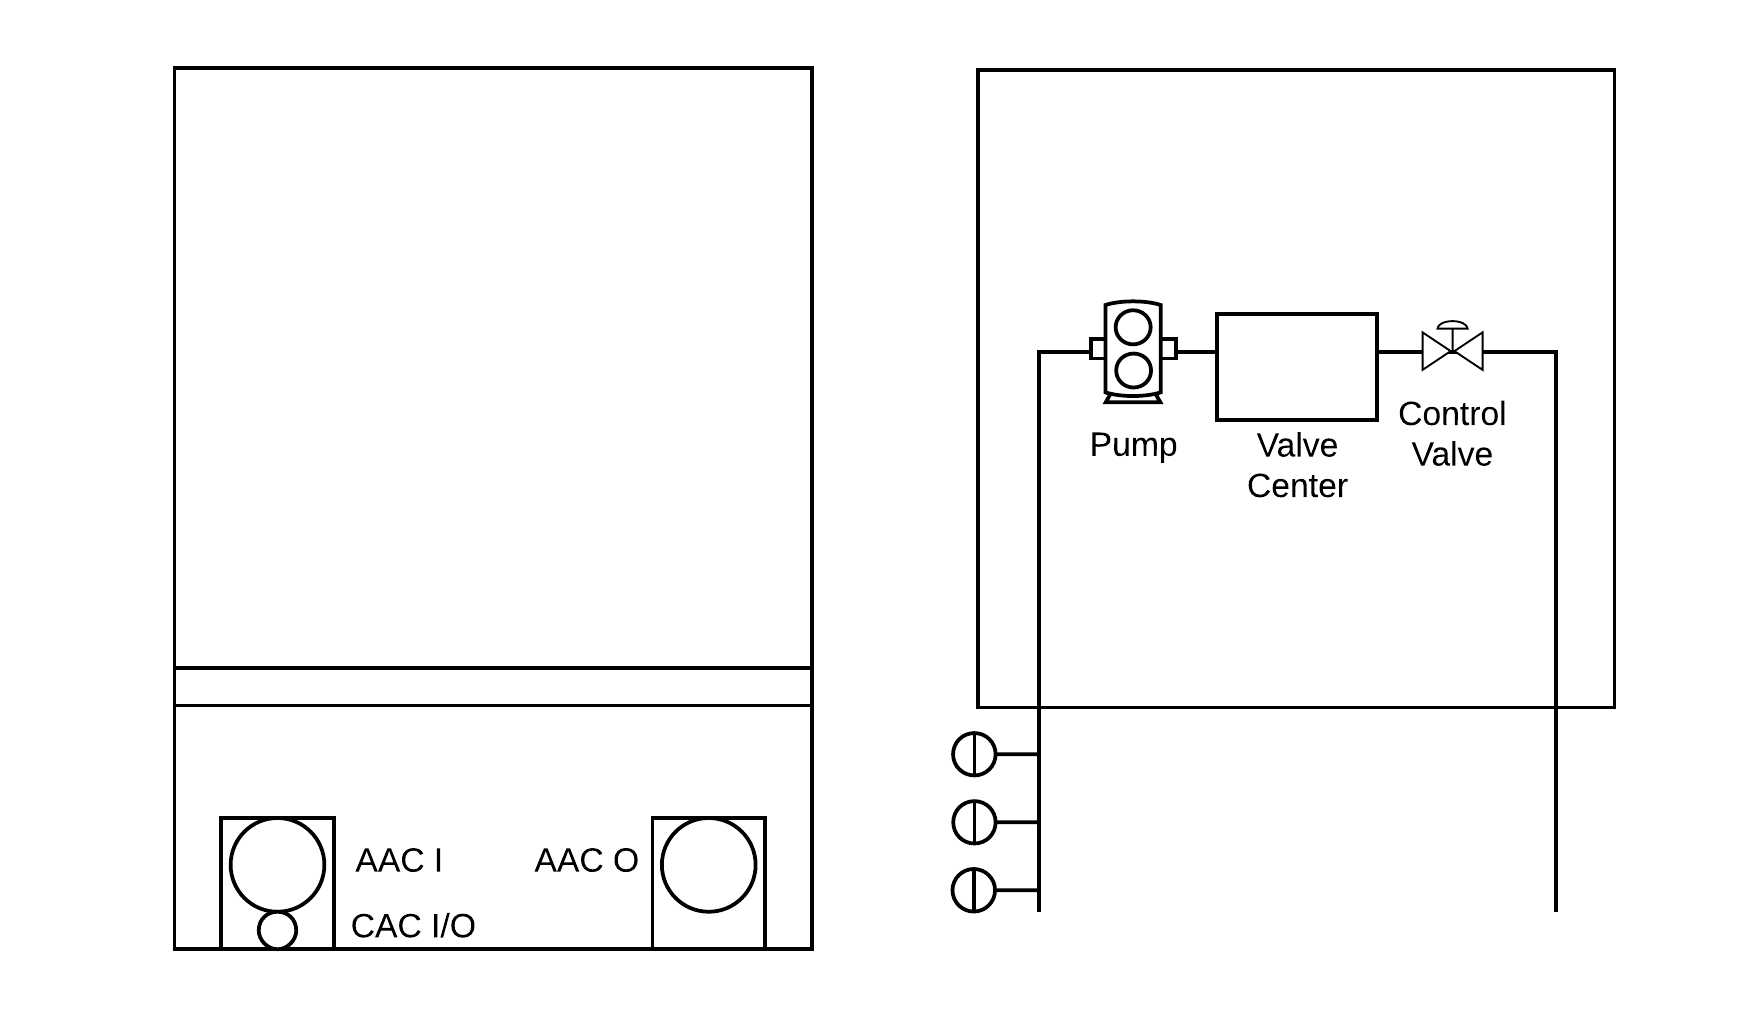
\includegraphics[width=0.7\textwidth]{4-experiment-design/img/Diagram_pipe.png}
    }\end{align*}
    %DIFAUXCMD
%DIFDELCMD < \caption{%
{%DIFAUXCMD
\DIFdelFL{Diagram of the experiment box face exposed to the outside.}}%DIFAUXCMD
%DIFDELCMD < \label{fig:pipes_interface_1}
%DIFDELCMD < \end{figure}
%DIFDELCMD < 

%DIFDELCMD < %%%
\DIFdelend \iffalse
\subsubsection{Radio Frequencies (Optional)}
\begin{centering}
Not required.
\end{centering}
\bigskip

\subsubsection{Thermal (Optional)}
\begin{centering}
Not required.
\end{centering}
\bigskip
\fi


\raggedbottom
\begin{landscape}
\subsection{Experiment Components}
\subsubsection{Electrical Components}

Table \ref{tab:electrical-components} shows all required electrical components with mass and price.




%DIF < 


\begin{longtable}{|m{0.03\textwidth}|m{0.3\textwidth}|m{0.25\textwidth}|m{0.05\textwidth}|m{0.1\textwidth}|m{0.3\textwidth}|m{0.15\textwidth}|m{0.08\textwidth}|}
    
\hline
\textbf{ID} & \textbf{Components} & \textbf{Specs (size,weight)} & \textbf{No.} & \textbf{Cost} & \textbf{Note} & \textbf{Availability} & \textbf{Status} \\ 
\hline
1 & Arduino Due & 101.52 mm x 53.3 mm, 36 g & 1 & 35 Euro & Fast and has many analog, and digital pins & Easily ordered online & Ordered \\ \hline
2 & W5500 Ethernet Shield  & 36 g & 1 & 28 Euro & Easily, connected on top of the board & Easily ordered online & Ordered \\ \hline
3 & KNF 850.1.2. KNDC B Miniature Diaphragm Pump & 30 x 54.3 x 77.5 mm, 430g  & 1 & 350 Euro & Low power, small size & Ordered online & Ordered \\ \hline
4 & Barometric Pressure Sensor MS5607-02BA03 & 5.0 x 3.0 x 1.0 mm, 1g  & 3 &  11 Euro & High resolution, large measuring range & Easily ordered online & To be ordered online \\ \hline
5 & Electromagnetically controlled valve & 1-1/2", 2640 g & 12 & 1756 Euro & Cascaded/series of valves & Easily ordered online & One ordered for testing \\ \hline
6 & Airflow sensor AWM40000 Series & 14 g & 1 & 106 Euro & good temperature range, high accuracy & Easily ordered online & To be ordered online \\ \hline
7 & Polyimide Thermofoil Heaters HK5161R78.4L12 & 12.7 x 101.6 mm, 6.84g & 1 & 40 Euro & Easy to mount, compact size & Easily ordered online & To be ordered online \\ \hline
8 & Polyimide Thermofoil Heaters HK5160R157L12 & 12.7 x 50.8 mm, 6.84g & 1 & 40 Euro & Easy to mount, compact size & Easily ordered online & To be ordered online \\ \hline
9 & Temperature sensor VSSOP-8, LM75A, Texas Instruments & 5.3 x 3.4 x 1.4 mm & 12 & 4 Euro & I2C digital output interface, temperature range down to - 55 ℃ & Easily ordered online & To be ordered online \\ \hline
10 & DC-DC Converter TEN 5 Series, 6 W, 12 V & 20.3 x 31.8 mm, 33.8 g & 3 & 50 Euro & Provides required output voltage and power & Easily ordered online & To be ordered online \\ \hline
11 & HDC2010 Low Power Humidity Digital Sensors & 1.5 x 1.5 x 0.675 mm, 15g & 1 & 3 Euro & I2C interface, good temperature range, high accuracy & Easily ordered online & To be ordered online \\ \hline
12 & Industrial temperature microSD XCUHS-I 8GB & 15 x 11 x 1 mm, 0.5 g & 1 & 20 Euro & Small, good temperature range, sufficient storage & Easily ordered online & Ordered  \\ \hline
13 & Logic CAT5E Network (2m) & 2 m, 90g & 1 & 7 Euro & Will be used for testing & Easily ordered in the nearest store & To be bought \\ \hline
14 & Electrical wires & 30g &  30 & 15 Eur & For use in testing and the final PCB board and circuitry & Easily ordered online & To be ordered \\ \hline
15 & Heat sinks & 25g &  5 &  5 Eur & For dissipating heat generated from components & Easily ordered online & To be ordered \\ \hline
16 & Resistors & 15g & 3 & 1.5 Eur & For use in valve switching circuit & Easily ordered online & To be ordered \\ \hline
17 & Transistors & 18g & 18 & 9 Eur &  For use in valve switching circuit & Easily ordered online & To be ordered \\ \hline 


    \caption{Table showing all required electrical components}
    \label{tab:electrical-components}
\end{longtable}
\raggedbottom
\DIFaddbegin \begin{longtable}{|m{0.03\textwidth}|m{0.3\textwidth}|m{0.25\textwidth}|m{0.05\textwidth}|m{0.1\textwidth}|m{0.3\textwidth}|m{0.15\textwidth}|m{0.08\textwidth}|}
    \DIFaddend 

\DIFdelbegin %DIFDELCMD < \begin{table}[H]
%DIFDELCMD <     %%%
\begin{align*}
        \DIFdelFL{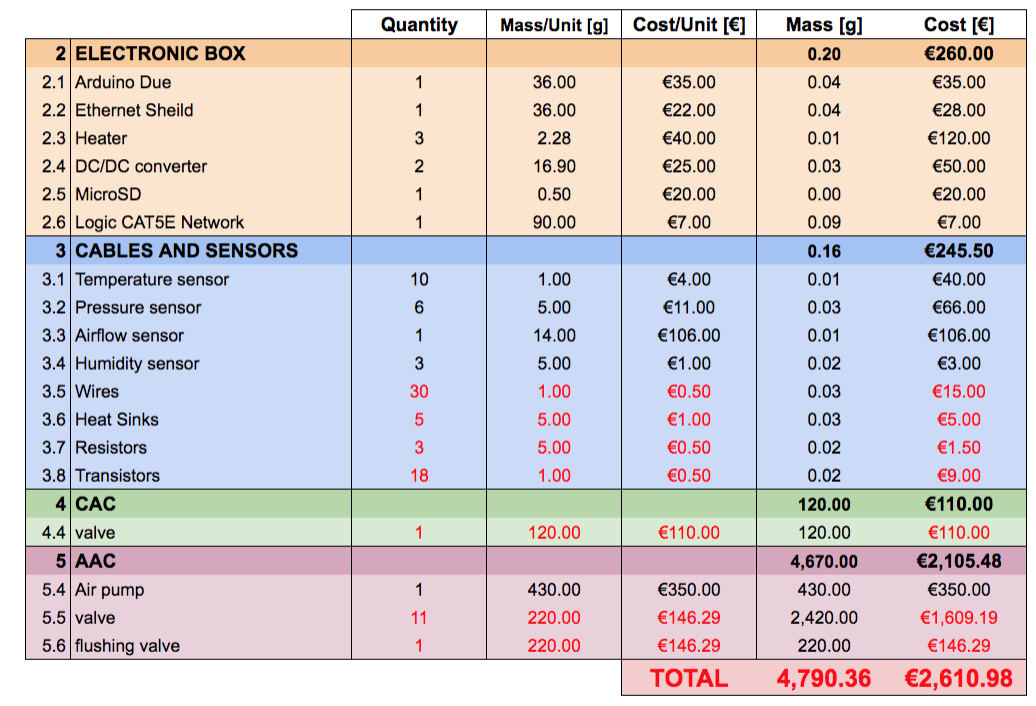
\includegraphics[height=10cm]{4-experiment-design/img/electrical-components-table.png}
    }\end{align*}
    %DIFAUXCMD
\DIFdelendFL \DIFaddbeginFL \hline
\textbf{\DIFaddFL{ID}} & \textbf{\DIFaddFL{Components}} & \textbf{\DIFaddFL{Specs (size,weight)}} & \textbf{\DIFaddFL{No.}} & \textbf{\DIFaddFL{Cost}} & \textbf{\DIFaddFL{Note}} & \textbf{\DIFaddFL{Availability}} & \textbf{\DIFaddFL{Status}} \\ 
\hline
\DIFaddFL{1 }& \DIFaddFL{Arduino Due }& \DIFaddFL{101.52 mm x 53.3 mm, 36 g }& \DIFaddFL{1 }& \DIFaddFL{35 Euro }& \DIFaddFL{Fast and has many analog, and digital pins }& \DIFaddFL{Easily ordered online }& \DIFaddFL{Ordered }\\ \hline
\DIFaddFL{2 }& \DIFaddFL{W5500 Ethernet Shield  }& \DIFaddFL{36 g }& \DIFaddFL{1 }& \DIFaddFL{28 Euro }& \DIFaddFL{Easily, connected on top of the board }& \DIFaddFL{Easily ordered online }& \DIFaddFL{Ordered }\\ \hline
\DIFaddFL{3 }& \DIFaddFL{KNF 850.1.2. KNDC B Miniature Diaphragm Pump }& \DIFaddFL{30 x 54.3 x 77.5 mm, 430g  }& \DIFaddFL{1 }& \DIFaddFL{350 Euro }& \DIFaddFL{Low power, small size }& \DIFaddFL{Ordered online }& \DIFaddFL{Ordered }\\ \hline
\DIFaddFL{4 }& \DIFaddFL{Barometric Pressure Sensor MS5607-02BA03 }& \DIFaddFL{5.0 x 3.0 x 1.0 mm, 1g  }& \DIFaddFL{3 }&  \DIFaddFL{11 Euro }& \DIFaddFL{High resolution, large measuring range }& \DIFaddFL{Easily ordered online }& \DIFaddFL{To be ordered online }\\ \hline
\DIFaddFL{5 }& \DIFaddFL{Electromagnetically controlled valve }& \DIFaddFL{1-1/2", 2640 g }& \DIFaddFL{12 }& \DIFaddFL{1756 Euro }& \DIFaddFL{Cascaded/series of valves }& \DIFaddFL{Easily ordered online }& \DIFaddFL{One ordered for testing }\\ \hline
\DIFaddFL{6 }& \DIFaddFL{Airflow sensor AWM40000 Series }& \DIFaddFL{14 g }& \DIFaddFL{1 }& \DIFaddFL{106 Euro }& \DIFaddFL{good temperature range, high accuracy }& \DIFaddFL{Easily ordered online }& \DIFaddFL{To be ordered online }\\ \hline
\DIFaddFL{7 }& \DIFaddFL{Polyimide Thermofoil Heaters HK5161R78.4L12 }& \DIFaddFL{12.7 x 101.6 mm, 6.84g }& \DIFaddFL{1 }& \DIFaddFL{40 Euro }& \DIFaddFL{Easy to mount, compact size }& \DIFaddFL{Easily ordered online }& \DIFaddFL{To be ordered online }\\ \hline
\DIFaddFL{8 }& \DIFaddFL{Polyimide Thermofoil Heaters HK5160R157L12 }& \DIFaddFL{12.7 x 50.8 mm, 6.84g }& \DIFaddFL{1 }& \DIFaddFL{40 Euro }& \DIFaddFL{Easy to mount, compact size }& \DIFaddFL{Easily ordered online }& \DIFaddFL{To be ordered online }\\ \hline
\DIFaddFL{9 }& \DIFaddFL{Temperature sensor VSSOP-8, LM75A, Texas Instruments }& \DIFaddFL{5.3 x 3.4 x 1.4 mm }& \DIFaddFL{12 }& \DIFaddFL{4 Euro }& \DIFaddFL{I2C digital output interface, temperature range down to - 55 ℃ }& \DIFaddFL{Easily ordered online }& \DIFaddFL{To be ordered online }\\ \hline
\DIFaddFL{10 }& \DIFaddFL{DC-DC Converter TEN 5 Series, 6 W, 12 V }& \DIFaddFL{20.3 x 31.8 mm, 33.8 g }& \DIFaddFL{3 }& \DIFaddFL{50 Euro }& \DIFaddFL{Provides required output voltage and power }& \DIFaddFL{Easily ordered online }& \DIFaddFL{To be ordered online }\\ \hline
\DIFaddFL{11 }& \DIFaddFL{HDC2010 Low Power Humidity Digital Sensors }& \DIFaddFL{1.5 x 1.5 x 0.675 mm, 15g }& \DIFaddFL{1 }& \DIFaddFL{3 Euro }& \DIFaddFL{I2C interface, good temperature range, high accuracy }& \DIFaddFL{Easily ordered online }& \DIFaddFL{To be ordered online }\\ \hline
\DIFaddFL{12 }& \DIFaddFL{Industrial temperature microSD XCUHS-I 8GB }& \DIFaddFL{15 x 11 x 1 mm, 0.5 g }& \DIFaddFL{1 }& \DIFaddFL{20 Euro }& \DIFaddFL{Small, good temperature range, sufficient storage }& \DIFaddFL{Easily ordered online }& \DIFaddFL{Ordered  }\\ \hline
\DIFaddFL{13 }& \DIFaddFL{Logic CAT5E Network (2m) }& \DIFaddFL{2 m, 90g }& \DIFaddFL{1 }& \DIFaddFL{7 Euro }& \DIFaddFL{Will be used for testing }& \DIFaddFL{Easily ordered in the nearest store }& \DIFaddFL{To be bought }\\ \hline
\DIFaddFL{14 }& \DIFaddFL{Electrical wires }& \DIFaddFL{30g }&  \DIFaddFL{30 }& \DIFaddFL{15 Eur }& \DIFaddFL{For use in testing and the final PCB board and circuitry }& \DIFaddFL{Easily ordered online }& \DIFaddFL{To be ordered }\\ \hline
\DIFaddFL{15 }& \DIFaddFL{Heat sinks }& \DIFaddFL{25g }&  \DIFaddFL{5 }&  \DIFaddFL{5 Eur }& \DIFaddFL{For dissipating heat generated from components }& \DIFaddFL{Easily ordered online }& \DIFaddFL{To be ordered }\\ \hline
\DIFaddFL{16 }& \DIFaddFL{Resistors }& \DIFaddFL{15g }& \DIFaddFL{3 }& \DIFaddFL{1.5 Eur }& \DIFaddFL{For use in valve switching circuit }& \DIFaddFL{Easily ordered online }& \DIFaddFL{To be ordered }\\ \hline
\DIFaddFL{17 }& \DIFaddFL{Transistors }& \DIFaddFL{18g }& \DIFaddFL{18 }& \DIFaddFL{9 Eur }&  \DIFaddFL{For use in valve switching circuit }& \DIFaddFL{Easily ordered online }& \DIFaddFL{To be ordered }\\ \hline 


    \DIFaddendFL \caption{Table showing all required electrical components\DIFdelbeginFL \DIFdelFL{.}\DIFdelendFL }
    \label{tab:electrical-components}
\DIFdelbeginFL %DIFDELCMD < \end{table}
%DIFDELCMD < %%%
\DIFdelend \DIFaddbegin \end{longtable}
\raggedbottom
\DIFaddend 

%DIF >  \begin{table}[H]
%DIF >      \begin{align*}
%DIF >          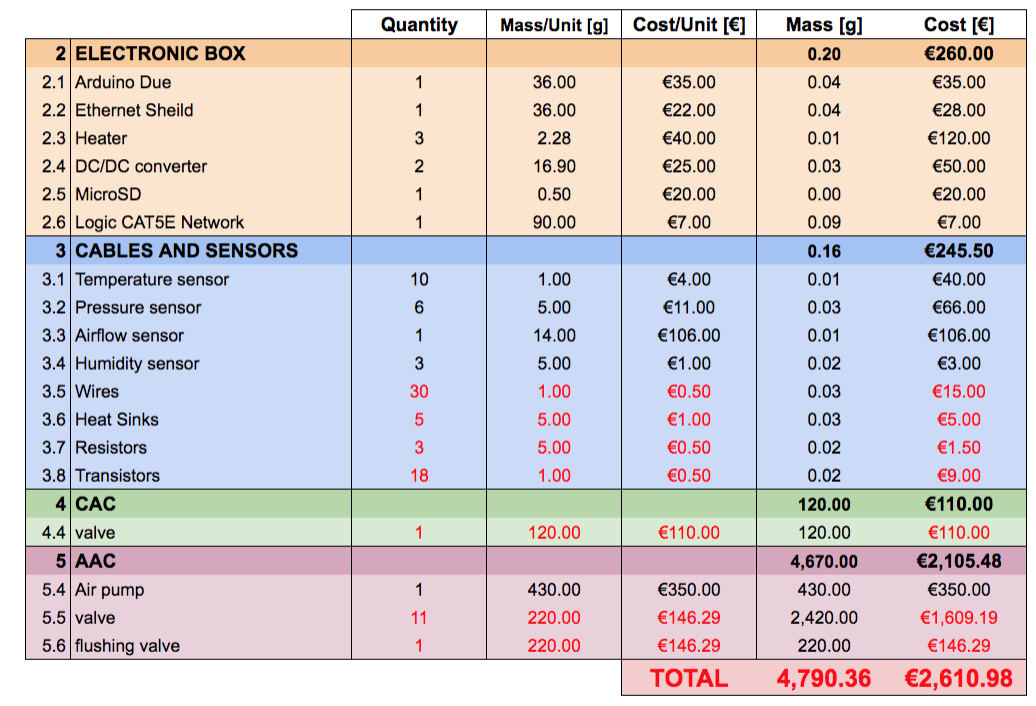
\includegraphics[height=10cm]{4-experiment-design/img/electrical-components-table.png}
%DIF >      \end{align*}
%DIF >      \caption{Table showing all required electrical components.}\label{tab:electrical-components}
%DIF >  \end{table}
\DIFaddbegin 

\DIFaddend \end{landscape}

\begin{landscape}

\subsubsection{Mechanical Components}

Table \ref{tab:mechanical-components} shows all required mechanical components with mass and price. Table cells highlighted in yellow denote values that have yet to be determined.

%DIF < \begin{longtable}{|m{0.03\textwidth}|m{0.2\textwidth}|m{0.25\textwidth}|m{0.05\textwidth}|m{0.1\textwidth}|m{0.28\textwidth}|m{0.15\textwidth}|m{0.15\textwidth}|}
     
   
\hline
\textbf{ID} & \textbf{Components} & \textbf{Specs (size,weight)} & \textbf{No.} & \textbf{Cost} & \textbf{Note} & \textbf{Availability} & \textbf{Status} \\ \hline
1 & Aluminum Bar & 45cm & 16 & TBD\footnote{Request for quotes have been sent to identified vendors and responses are still pending. \label{fn:mechcomp1}} & Railed geometry, Structural element & Online & To be ordered \\ \hline
2 & Aluminum Bar & 40cm & 4 & TBD\textsuperscript{\ref{fn:mechcomp1}} & Railed geometry, Structural element & Online & To be ordered \\ \hline
3 & Aluminum Bar & 25cm & 4 & TBD\textsuperscript{\ref{fn:mechcomp1}} & Railed geometry, Structural element & Online & To be ordered \\ \hline
4 & Aluminum Plate & 50 x 40 x 0.2 cm & 4 & TBD\footnote{The other elements still need to be found either in the store or online. \label{fn:mechcomp2}} & Wall, Protective element & Store & To be ordered \\ \hline
5 & Aluminum Plate & 50 x 25 x 0.2 cm & 4 & TBD\textsuperscript{\ref{fn:mechcomp2}} & Wall, Protective element & Store & To be ordered \\ \hline
6 & Aluminum Plate & 50 x 50 x 0.2 cm & 2 & TBD\textsuperscript{\ref{fn:mechcomp2}} & Wall, Protective element & Store & To be ordered \\ \hline
7 & Styrofoam & 2 $m^2$, 2.5cm thick & 1 & TBD\textsuperscript{\ref{fn:mechcomp2}} & Wall, Protective element & Store & To be ordered \\ \hline
8 & Bag Valves & \textit{Swagelok} & 16 & TBD\textsuperscript{\ref{fn:mechcomp1}} & Interface bags with tubes & Online & To be ordered \\ \hline
9 & 90-degree angle & 0.25 x 0.25 cm & 52 & TBD\textsuperscript{\ref{fn:mechcomp2}} & Join structure bars & Online & To be ordered \\ \hline
10 & Coated box & 10 x 10 x 3 cm & 1 & TBD\textsuperscript{\ref{fn:mechcomp2}} & Valve center for AAC & Store & To be built \\ \hline
11 & Plastic Tube & 5 m & 1 & TBD\textsuperscript{\ref{fn:mechcomp2}} & Valves to bags & Store & To be ordered \\ \hline
12 & Air Filter & TBD\textsuperscript{\ref{fn:mechcomp2}} & 1 & TBD\textsuperscript{\ref{fn:mechcomp2}} & Main pipe protection & Store & To be built \\ \hline
13 & Flange & Small & 50 & TBD\textsuperscript{\ref{fn:mechcomp2}} & Join tubes with valves & Store & To be ordered \\ \hline
14 & Hinges & 5 x 5 x 0.1 cm & 2 & TBD\textsuperscript{\ref{fn:mechcomp2}} & Allow opening mechanism & Store & To be ordered \\ \hline
15 & Bar & 52.4 x 0.8 cm & 4 & TBD\textsuperscript{\ref{fn:mechcomp2}} & Anchor point fro bags & Store & To be ordered \\ \hline
16 & Handle & TBD\textsuperscript{\ref{fn:mechcomp2}} & 4 & TBD\textsuperscript{\ref{fn:mechcomp2}} & Experiment box manipulation & Store & To be ordered \\ \hline

    \caption{Table showing all required mechanical components}
    \label{tab:mechanical-components}
\end{longtable}
\raggedbottom
\DIFaddbegin \begin{longtable}{|m{0.03\textwidth}|m{0.2\textwidth}|m{0.25\textwidth}|m{0.05\textwidth}|m{0.1\textwidth}|m{0.28\textwidth}|m{0.15\textwidth}|m{0.15\textwidth}|}
     \DIFaddend 

   
\DIFdelbegin %DIFDELCMD < \begin{table}[H]
%DIFDELCMD <     %%%
\begin{align*}
        \DIFdelFL{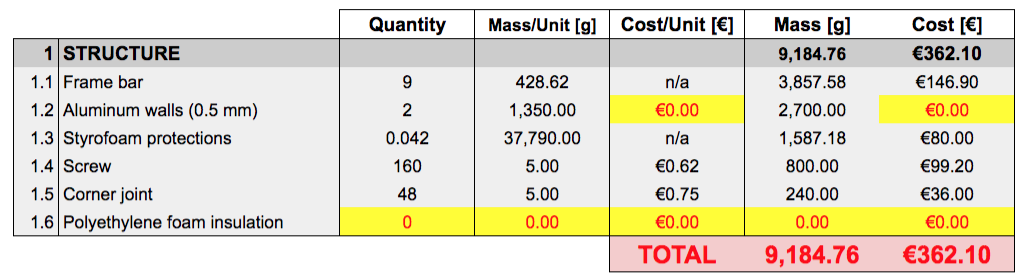
\includegraphics{4-experiment-design/img/mechanical-components-table.png}
    }\end{align*}
    %DIFAUXCMD
\DIFdelendFL \DIFaddbeginFL \hline
\textbf{\DIFaddFL{ID}} & \textbf{\DIFaddFL{Components}} & \textbf{\DIFaddFL{Specs (size,weight)}} & \textbf{\DIFaddFL{No.}} & \textbf{\DIFaddFL{Cost}} & \textbf{\DIFaddFL{Note}} & \textbf{\DIFaddFL{Availability}} & \textbf{\DIFaddFL{Status}} \\ \hline
\DIFaddFL{1 }& \DIFaddFL{Aluminum Bar }& \DIFaddFL{45cm }& \DIFaddFL{12 }& \DIFaddFL{TBD}\footnote{\DIFaddFL{Budget in Table 3.3.2 has estimated values. TBD here until exact values are figured out. }\label{fn:mechcomp1}} & \DIFaddFL{Railed geometry, Structural element }& \DIFaddFL{Online }& \DIFaddFL{To be ordered }\\ \hline
\DIFaddFL{2 }& \DIFaddFL{Aluminum Bar }& \DIFaddFL{40cm }& \DIFaddFL{8 }& \DIFaddFL{TBD\textsuperscript{\ref{fn:mechcomp1}} }& \DIFaddFL{Railed geometry, Structural element }& \DIFaddFL{Online }& \DIFaddFL{To be ordered }\\ \hline
\DIFaddFL{3 }& \DIFaddFL{Aluminum Bar }& \DIFaddFL{25cm }& \DIFaddFL{4 }& \DIFaddFL{TBD\textsuperscript{\ref{fn:mechcomp1}} }& \DIFaddFL{Railed geometry, Structural element }& \DIFaddFL{Online }& \DIFaddFL{To be ordered }\\ \hline
\DIFaddFL{4 }& \DIFaddFL{Aluminum Plate }& \DIFaddFL{50 x 40 x 0.2 cm }& \DIFaddFL{4 }& \DIFaddFL{TBD\textsuperscript{\ref{fn:mechcomp1}} }& \DIFaddFL{Wall, Protective element }& \DIFaddFL{Store }& \DIFaddFL{To be ordered }\\ \hline
\DIFaddFL{5 }& \DIFaddFL{Aluminum Plate }& \DIFaddFL{50 x 25 x 0.2 cm }& \DIFaddFL{4 }& \DIFaddFL{TBD\textsuperscript{\ref{fn:mechcomp1}} }& \DIFaddFL{Wall, Protective element }& \DIFaddFL{Store }& \DIFaddFL{To be ordered }\\ \hline
\DIFaddFL{6 }& \DIFaddFL{Aluminum Plate }& \DIFaddFL{50 x 50 x 0.2 cm }& \DIFaddFL{2 }& \DIFaddFL{TBD\textsuperscript{\ref{fn:mechcomp1}} }& \DIFaddFL{Wall, Protective element }& \DIFaddFL{Store }& \DIFaddFL{To be ordered }\\ \hline
\DIFaddFL{7 }& \DIFaddFL{Aluminum Plate }& \DIFaddFL{40 x 40 x 0.2 cm }& \DIFaddFL{2 }& \DIFaddFL{TBD\textsuperscript{\ref{fn:mechcomp1}} }& \DIFaddFL{Wall, Protective element }& \DIFaddFL{Store }& \DIFaddFL{To be ordered }\\ \hline
\DIFaddFL{8 }& \DIFaddFL{Styrofoam }& \DIFaddFL{2 \mbox{%DIFAUXCMD
$m^2$
}%DIFAUXCMD
, 1cm thick }& \DIFaddFL{1 }& \DIFaddFL{TBD\textsuperscript{\ref{fn:mechcomp1}} }& \DIFaddFL{Wall, Protective element }& \DIFaddFL{Store }& \DIFaddFL{To be ordered }\\ \hline
\DIFaddFL{9 }& \DIFaddFL{Polyethylene foam }& \DIFaddFL{2 \mbox{%DIFAUXCMD
$m^2$
}%DIFAUXCMD
, 1cm thick }& \DIFaddFL{1 }& \DIFaddFL{TBD\textsuperscript{\ref{fn:mechcomp1}} }& \DIFaddFL{Wall, Thermal insulation }& \DIFaddFL{Store }& \DIFaddFL{To be ordered }\\ \hline
%DIF > 9 & Bag Valves & \textit{Swagelok} & 16 & TBD\textsuperscript{\ref{fn:mechcomp1}} & Interface bags with tubes & Online & To be ordered \\ \hline
\DIFaddFL{10 }& \DIFaddFL{Corner joint }& \DIFaddFL{0.2 x 0.2 cm }& \DIFaddFL{52 }& \DIFaddFL{TBD\textsuperscript{\ref{fn:mechcomp1}} }& \DIFaddFL{Join structure bars, 90-degree angle }& \DIFaddFL{Online }& \DIFaddFL{To be ordered }\\ \hline
%DIF > 11 & Electronics shielding box & 20 x 10 x 10 cm & 1 & TBD\textsuperscript{\ref{fn:mechcomp2}} & Electronics center & Store & To be built \\ \hline
%DIF > 11 & Coated box & 20 x 10 x 10 cm & 1 & TBD\textsuperscript{\ref{fn:mechcomp2}} & Valve center for AAC & Store & To be built \\ \hline
%DIF > 12 & Plastic Tube & 5 m & 1 & TBD\textsuperscript{\ref{fn:mechcomp2}} & Valves to bags & Store & To be ordered \\ \hline
%DIF > 13 & Air Filter & TBD\textsuperscript{\ref{fn:mechcomp2}} & 1 & TBD\textsuperscript{\ref{fn:mechcomp2}} & Main pipe protection & Store & To be built \\ \hline
\DIFaddFL{11 }& \DIFaddFL{Flange }& \DIFaddFL{Small }& \DIFaddFL{50 }& \DIFaddFL{TBD\textsuperscript{\ref{fn:mechcomp1}} }& \DIFaddFL{Join tubes with valves }& \DIFaddFL{Store }& \DIFaddFL{To be ordered }\\ \hline
\DIFaddFL{12 }& \DIFaddFL{Bar }& \DIFaddFL{45 x 0.8 cm }& \DIFaddFL{2 }& \DIFaddFL{TBD\textsuperscript{\ref{fn:mechcomp1}} }& \DIFaddFL{Anchor point fro bags }& \DIFaddFL{Store }& \DIFaddFL{To be ordered }\\ \hline
\DIFaddFL{13 }& \DIFaddFL{Handle }& \DIFaddFL{TBD}\footnote{\DIFaddFL{Exact size depending on availability. }\label{fn:mechcomp2}} & \DIFaddFL{4 }& \DIFaddFL{TBD\textsuperscript{\ref{fn:mechcomp1}} }& \DIFaddFL{Experiment box manipulation }& \DIFaddFL{Store }& \DIFaddFL{To be ordered }\\ \hline
\DIFaddFL{14 }& \DIFaddFL{Screw }& \DIFaddFL{TBD\textsuperscript{\ref{fn:mechcomp2}} }& \DIFaddFL{160 }& \DIFaddFL{TBD\textsuperscript{\ref{fn:mechcomp1}} }& \DIFaddFL{Fixing elements }& \DIFaddFL{Store }& \DIFaddFL{To be ordered }\\ \hline

    \DIFaddendFL \caption{Table showing all required mechanical components\DIFdelbeginFL \DIFdelFL{.}\DIFdelendFL }
    \label{tab:mechanical-components}
\DIFdelbeginFL %DIFDELCMD < \end{table}
%DIFDELCMD < %%%
\DIFdelend \DIFaddbegin \end{longtable}
\raggedbottom
\DIFaddend 

%DIF > \begin{table}[H]
%DIF > %    \begin{align*}
%DIF >         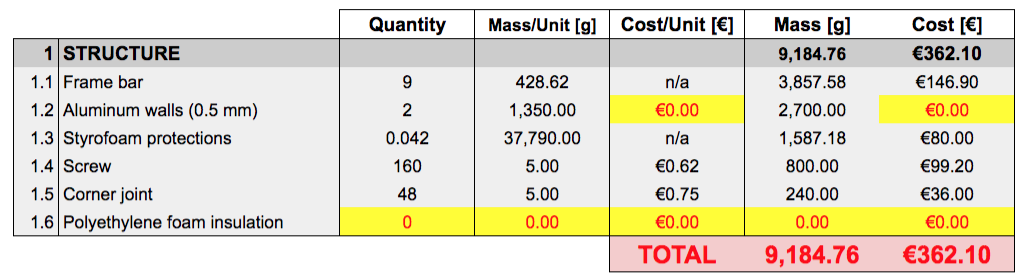
\includegraphics{4-experiment-design/img/mechanical-components-table.png}
%DIF >     \end{align*}
%DIF >     \caption{Table showing all required mechanical components.}\label{tab:mechanical-components}
%DIF > \end{table}
\DIFaddbegin 

\end{landscape}

\DIFaddend \subsubsection{Other Components}

Other components are included in the full budget previously presented in Table \ref{tab:budget-table}.


\DIFdelbegin %DIFDELCMD < \end{landscape}
%DIFDELCMD < 

%DIFDELCMD < %%%
\DIFdelend \raggedbottom
\pagebreak
\subsection{Mechanical Design} \label{Mechanical_Design}


\subsubsection{Structure}

The experiment consists on two cubic boxes, one stacked next to the other. The smallest box \DIFaddbegin \DIFadd{-in red in Figure \ref{overview}- }\DIFaddend allocates the heaviest element, the CAC. The main \DIFdelbegin \DIFdel{box }\DIFdelend \DIFaddbegin \DIFadd{box-in grey in Figure \ref{overview}- }\DIFaddend contains the AAC system as well as the general Electronic Box (EB). The frame of these two boxes will be made of aluminum bars which have a characteristic cross-section of 20x20 mm, see Figure \ref{cross-section}. The rails will allow an easy interface between bars and other elements. Bars will be joined together by using 90-degree angles \DIFaddbegin \DIFadd{and corner cubes}\DIFaddend , see Figure \ref{3_bars_joined}.

%% Cross section of one aluminum bar

\begin{figure}[!ht]
    \centering
    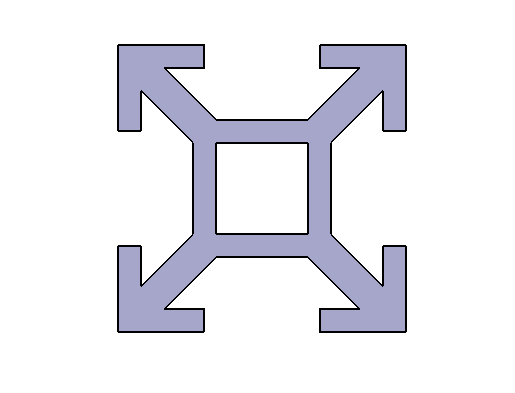
\includegraphics[width=0.5\textwidth]{4-experiment-design/img/1_cross_section.jpg}
    \caption{Cross section of the structural bars.}
    \label{cross-section}
\end{figure}

% Figure of 3 bars

\begin{figure}[!ht]
    \centering
    \DIFdelbeginFL %DIFDELCMD < 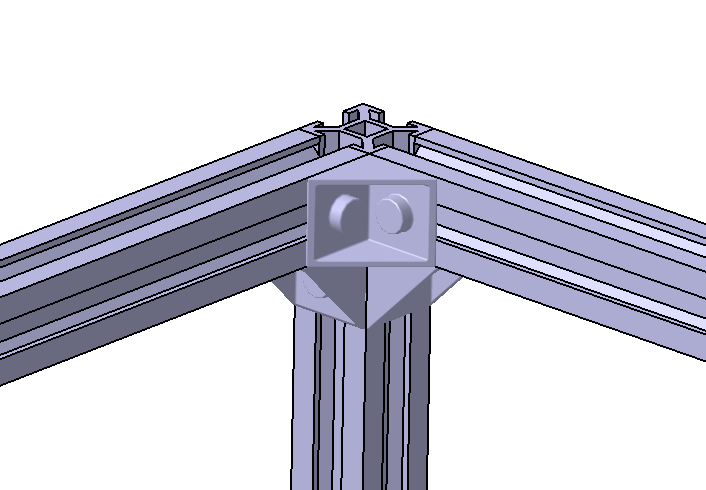
\includegraphics[width=0.6\textwidth]{4-experiment-design/img/bars_joint.jpg}
%DIFDELCMD <     %%%
\DIFdelendFL \DIFaddbeginFL 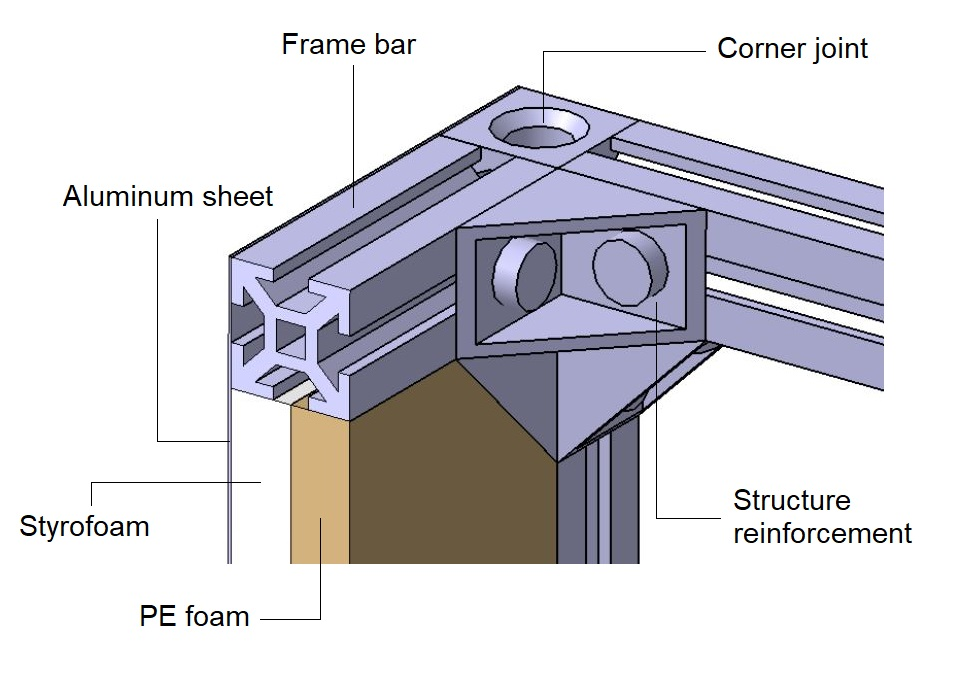
\includegraphics[width=0.8\textwidth]{4-experiment-design/img/structure_cut_name.jpg}
    \DIFaddendFL \caption{Interface between structural bars.}
    \label{3_bars_joined}
\end{figure}

The frame is designed to withstand all vibrations and ensure a reliable stability of the entire system. Further tests will help to confirm and update the design if necessary. 

The two-box design will allow ease of access and manipulation of both the CAC and AAC subsystems, see Figure \DIFdelbegin \DIFdel{\ref{strucutre}}\DIFdelend \DIFaddbegin \DIFadd{\ref{overview}}\DIFaddend . In addition, the AAC sampling system is designed to be re-usable for future handover to FMI, as such, it will be mountable on any standard balloon flight without having to introduce major design changes. The latter would imply to introduce a battery as a power unit, hence less bags could be carried (around \DIFdelbegin \DIFdel{8 bagsin the new setup)}\DIFdelend \DIFaddbegin \DIFadd{6 bags) in this potential future setup}\DIFaddend .

%DIF <  Figure of the two structures one above the other one (slightly separated)
%DIF >  Figure of the two structures
%DIF > \begin{figure}[!ht]
%DIF >     \centering
%DIF >     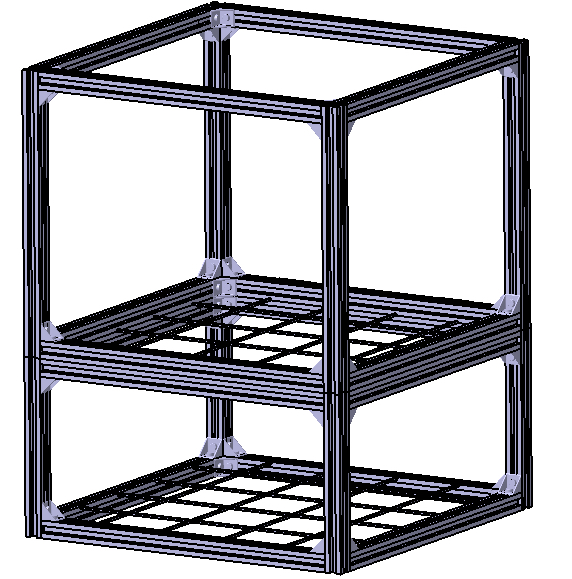
\includegraphics[width=0.7\textwidth, angle=90]{4-experiment-design/img/frame_structure.jpg}
%DIF >     \caption{Structure of the two-box design.}
%DIF >     \label{strucutre}
%DIF > \end{figure}
\DIFaddbegin 

\DIFaddend \begin{figure}[!ht]
    \centering
    \DIFdelbeginFL %DIFDELCMD < 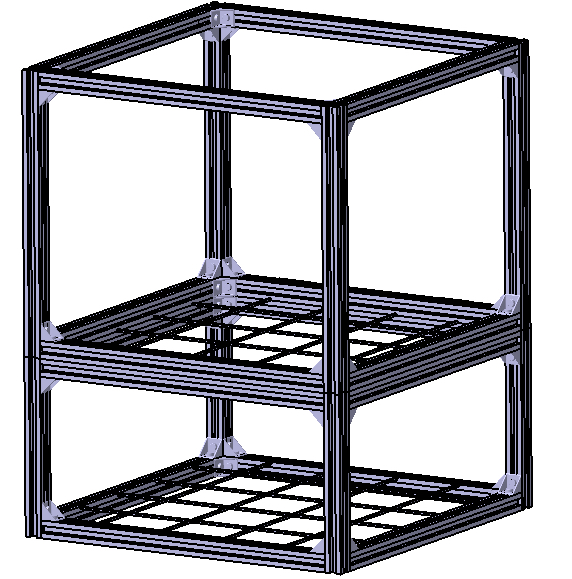
\includegraphics[width=0.7\textwidth, angle=90]{4-experiment-design/img/frame_structure.jpg}
%DIFDELCMD <     %%%
\DIFdelendFL \DIFaddbeginFL 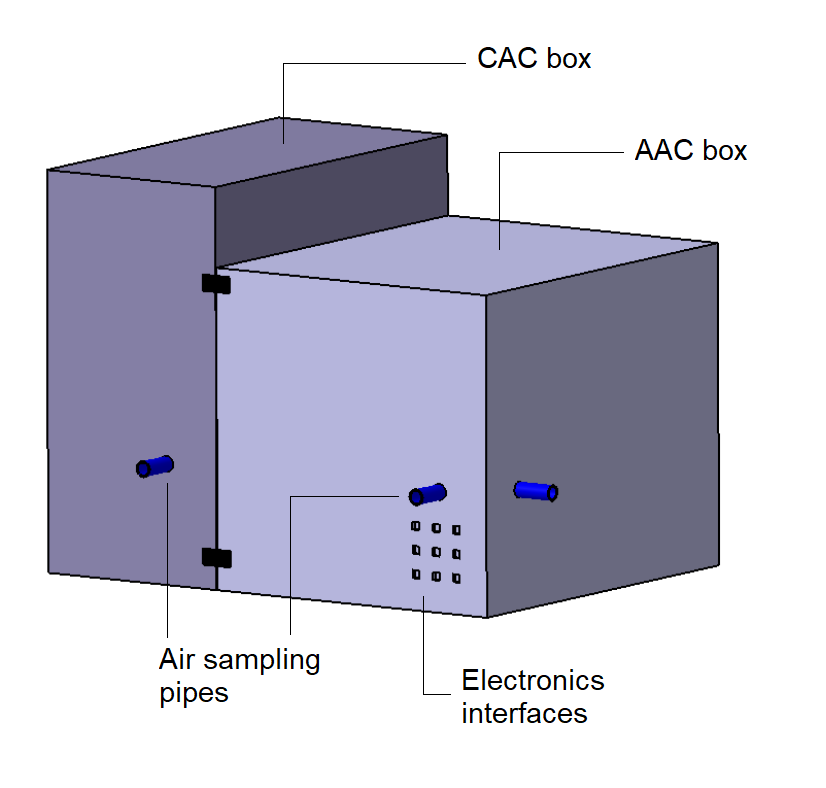
\includegraphics[width=0.7\textwidth]{4-experiment-design/img/overview_names.png}
    \DIFaddendFL \caption{\DIFdelbeginFL \DIFdelFL{Structure }\DIFdelendFL \DIFaddbeginFL \DIFaddFL{General configuration }\DIFaddendFL of the \DIFdelbeginFL \DIFdelFL{two-box design}\DIFdelendFL \DIFaddbeginFL \DIFaddFL{experiment}\DIFaddendFL .}
    \DIFdelbeginFL %DIFDELCMD < \label{strucutre}
%DIFDELCMD < %%%
\DIFdelendFL \DIFaddbeginFL \label{overview}
\DIFaddendFL \end{figure}

\subsubsection{CAC Subsystem}

The CAC subsystem is designed \DIFdelbegin \DIFdel{with }\DIFdelend \DIFaddbegin \DIFadd{to fit }\DIFaddend a 300-meter coiled tube, the valve governing it and a temperature sensor. To determine its positioning inside the gondola and the experiment box, some mechanical issues \DIFaddbegin \DIFadd{and gondola constraints }\DIFaddend must be considered.

\smallskip
Firstly, it is possible to identify the interface to attach the experiment box to the gondola as one of the most critical points in terms of mechanics performance. In the worst case scenario, with a heavy experiment and without a proper study of the aforesaid interface, shear in the screws could be produced after a violent landing stress. Since the CAC will be the heaviest component in the whole experiment, its location and orientation will affect directly the stress analysis of the structure. The larger the distance to the fixed points, the bigger the \DIFdelbegin \DIFdel{Momentum }\DIFdelend \DIFaddbegin \DIFadd{momentum }\DIFaddend produced by the component. Nevertheless, due to fast recovery implementation, the CAC tube will be placed vertically. Therefore, its dedicated box will be properly attached to the AAC box by means of 4 anchor points\DIFaddbegin \DIFadd{, in blacb in Figure \ref{overview}}\DIFaddend . The fast recovery then will only imply unscrewing 4 screws and \DIFdelbegin \DIFdel{disconnect }\DIFdelend \DIFaddbegin \DIFadd{disconnecting }\DIFaddend a wire. 

\smallskip
In order to command the valve, a wire will go out from the box and \DIFdelbegin \DIFdel{plugged on }\DIFdelend \DIFaddbegin \DIFadd{connected to }\DIFaddend the electronics interface panel located on an AAC box wall.

\smallskip
In addition, to avoid sample contamination with standstill air inside the gondola, the coil will have a direct outside inlet and outlet by means of an extension tube reaching further from the gondola’s limits\DIFaddbegin \DIFadd{, in blue in the red box in Figure \ref{overview}}\DIFaddend .


\DIFdelbegin %DIFDELCMD < \pagebreak
%DIFDELCMD < %%%
\DIFdelend \subsubsection{AAC Subsystem}

The AAC Subsystem consists of \DIFdelbegin \DIFdel{10 }\DIFdelend \DIFaddbegin \DIFadd{7 }\DIFaddend three-liter sampling bags. Each bag will have a dedicated valve in the Valve Center (VC) to allow emptying and filling processes as well as to close the bag when needed. The bags will be placed vertically and will have two anchor points: on the top through a  multiple anchor interface (see Figure \ref{anchor_bags}) and on the bottom by means of the tubes connecting them to the valves.

%% Several Figures of the top box with its inside elements: isometric, top view and front view.

\begin{figure}[!ht]
    \centering
    \DIFdelbeginFL %DIFDELCMD < 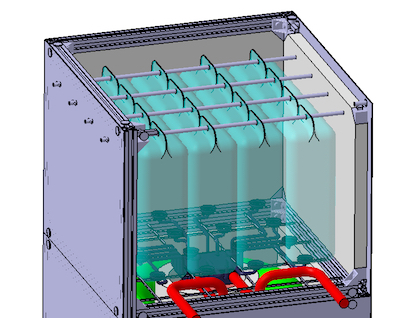
\includegraphics[width=0.7\textwidth]{4-experiment-design/img/anchored_bags.jpg}
%DIFDELCMD <     %%%
\DIFdelendFL \DIFaddbeginFL 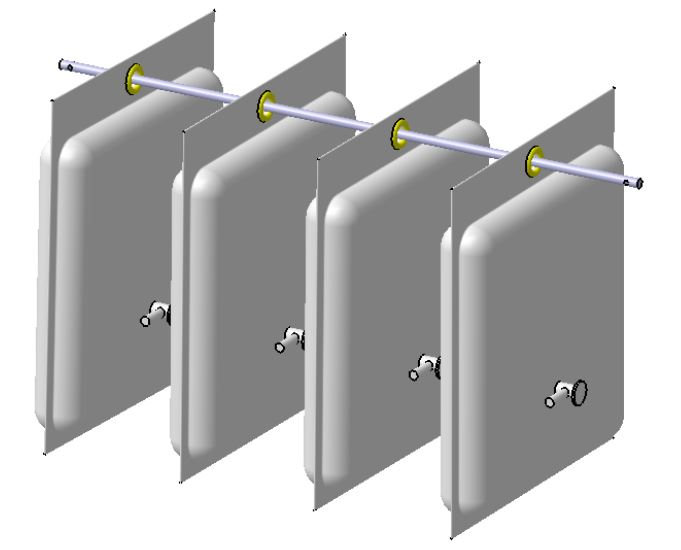
\includegraphics[width=0.7\textwidth]{4-experiment-design/img/bags_assembly.jpg}
    \DIFaddendFL \caption{\DIFdelbeginFL \DIFdelFL{AAC Subsystem }\DIFdelendFL \DIFaddbeginFL \DIFaddFL{Sampling bags }\DIFaddendFL with \DIFdelbeginFL \DIFdelFL{all its elements}\DIFdelendFL \DIFaddbeginFL \DIFaddFL{fixing interface}\DIFaddendFL .}
    \label{anchor_bags}
\end{figure}

\DIFdelbegin %DIFDELCMD < \pagebreak
%DIFDELCMD < %%%
\DIFdelend \subsubsection{Electronics Box}

The OBC and its external elements will be allocated in a bottom corner of the experiment box, inside AAC box, and on the opposite side of the CAC box. \DIFdelbegin \DIFdel{The latter }\DIFdelend \DIFaddbegin \DIFadd{This }\DIFaddend will allow an easy access and manipulation as well as the required external interfaces\DIFaddbegin \DIFadd{, holes in Figure \ref{overview}}\DIFaddend . The smallest side of the EB will have the outer connections interfaces. Hence, the wall will have the necessary holes. The EB will be fixed to the AAC box structure bars in 3 different points.


%% Figure of the electronics box inside the coil, only bottom cube, isometric top view, explosion

%\begin{figure}[!ht]
 %   \centering
  %  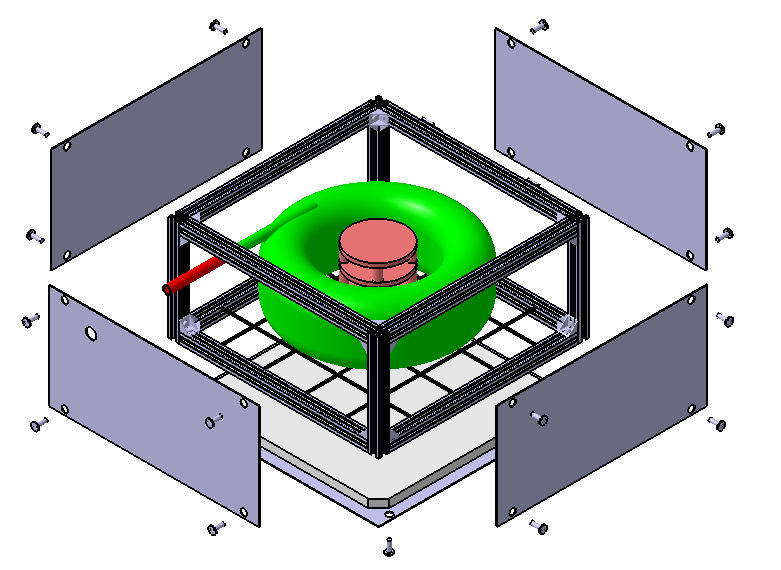
\includegraphics[width=0.7\textwidth]{4-experiment-design/img/explos_CAC.jpg}
   % \caption{.}
    %\label{electronics_box}
%\end{figure}

\pagebreak
\subsubsection{Valve Center}

The valve center consists of a coated box to which the AAC's \DIFdelbegin \DIFdel{10 }\DIFdelend \DIFaddbegin \DIFadd{7 }\DIFaddend air sampling bags will be attached to. This box will serve as \DIFdelbegin \DIFdel{the air flow }\DIFdelend \DIFaddbegin \DIFadd{airflow }\DIFaddend chamber. It will be connected to a pipe from which outside air will be pumped and also enable pre-sample collection flushing\DIFdelbegin \DIFdel{, see Figure \ref{valve_center_and_pipes}}\DIFdelend . The pump providing the airflow will be allocated on the inlet side and protected by an air filter. It will be allocated inside a shielding box, more detailed information in section \ref{Thermal_section}. \DIFaddbegin \DIFadd{The pipes used for both intake and outlet can be seen in blue in the grey box in Figure \ref{overview}.
}\DIFaddend 

\smallskip
Both the pump box and the valve center will be allocated above the EB so all the command center is at the same place. Having them together will provide as well a proper cooling system monitored by several temperature sensors. \DIFdelbegin \DIFdel{A sketch of the setup can be seen in Figure ....
}\DIFdelend %DIF > A sketch of the setup can be seen in Figure ....

%% Figure of the valve center with the pipe and small tubes

%\begin{figure}[!ht]
%    \centering
%    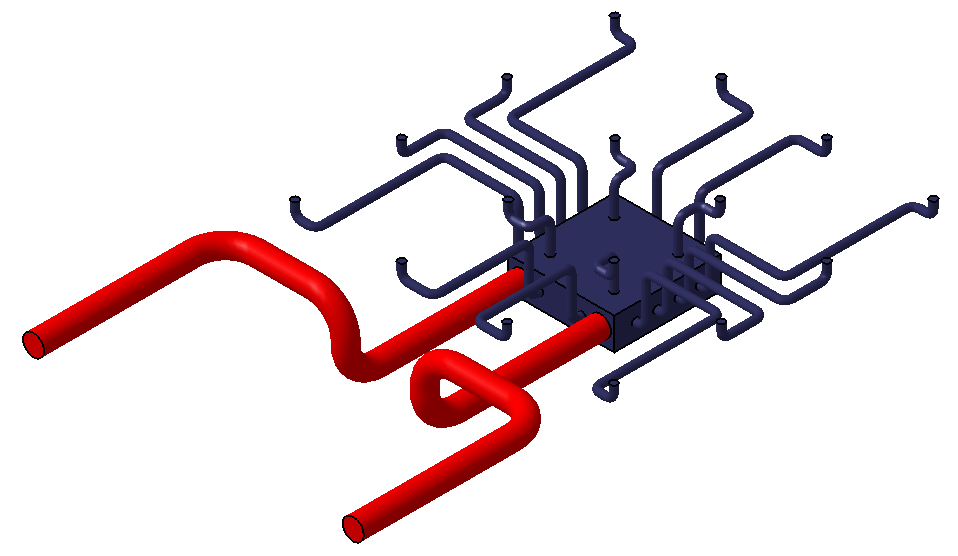
\includegraphics[width=0.9\textwidth]{4-experiment-design/img/valve_collector.jpg}
%    \caption{Valve center with all the tubes to the sampling bags and to the outside environment.}
%    \label{valve_center_and_pipes}
%\end{figure}

%% Add figure with EB and external interface + VC + Pump Box + Pipes + fixing elements


\DIFdelbegin %DIFDELCMD < \pagebreak
%DIFDELCMD < %%%
\DIFdelend \subsubsection{Protection}

In order to protect the components from all kind of external elements, the experiment box will be shielded with removable aluminum walls along with a thick layer of Styrofoam combined with Polyethylene foam attached to each wall. No internal space will be lost since the \DIFaddbegin \DIFadd{total }\DIFaddend foam thickness is the same as that of the structural bars. Isolating sheets will also be glued in the walls to reinforce the temperature shielding.
%DIF < Each box has an internal aluminum mesh at the bottom face. It will help to protect the CAC coiled tube from impacts as well as to withstand its considerable mass. On the other hand, the mesh in the upper box is used to fix the valve center at a privileged centered position.

The walls will properly protect both the CAC coiled tube and the AAC sampling bags from any external element, unexpected rapid movements, and a probable hard landing impact.
\DIFdelbegin \DIFdel{Cross-section in Figure \ref{cut_all}. 
}\DIFdelend %DIF > see in Figure \ref{walls}. 


%DIF < % Cut: Figure CAC+EB, AAC+valve center, and walls + Styrofoam.
%DIF > % Cut: Figure CAC+EB, AAC+valve center, and walls + Styrofoam. Label all the parts

\DIFdelbegin %DIFDELCMD < \begin{figure}[!ht]
%DIFDELCMD <     \centering
%DIFDELCMD <     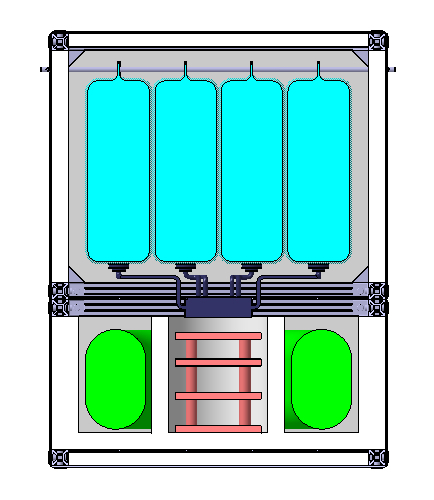
\includegraphics[width=0.7\textwidth]{4-experiment-design/img/tall_frontal.jpg}
%DIFDELCMD <     %%%
%DIFDELCMD < \caption{%
{%DIFAUXCMD
\DIFdelFL{Cross-section of the whole experiment box.}}
    %DIFAUXCMD
%DIFDELCMD < \label{cut_all}
%DIFDELCMD < \end{figure}
%DIFDELCMD < %%%
\DIFdelend %DIF > \begin{figure}[!ht]
%DIF >     \centering
%DIF >     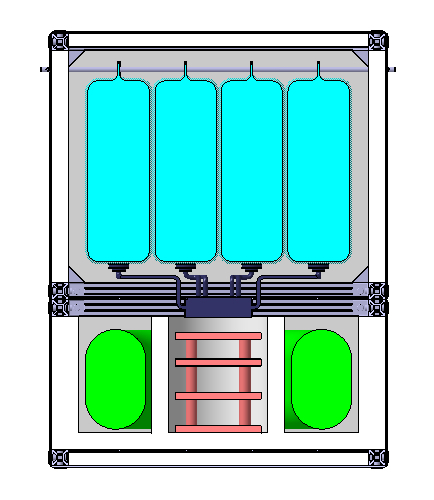
\includegraphics[width=0.2\textwidth]{4-experiment-design/img/tall_frontal.jpg}
%DIF >     \caption{Wall layers.}
%DIF >     \label{walls}
%DIF > \end{figure}

The front walls, face of the experiment box exposed to the outside, will have several holes\DIFaddbegin \DIFadd{: }\DIFaddend to allow the tubes providing air flow to collect clean air from the outside, \DIFdelbegin \DIFdel{see Figure \ref{front_wall_holes}}\DIFdelend \DIFaddbegin \DIFadd{and to manipulate the electric connections}\DIFaddend .

%The top lateral walls will have four holes to allow the introduction of the circular bars used as anchor points for the sampling bags, see Figure \ref{anchor_bags}.

Bolts shall be used to attach all walls to the structure's railed bars.

%DIF < % Figure front wall holes: isometric
%DIF > % Figure front wall holes: isometric Include labels

\DIFdelbegin %DIFDELCMD < \begin{figure}[!ht]
%DIFDELCMD <     \centering
%DIFDELCMD <     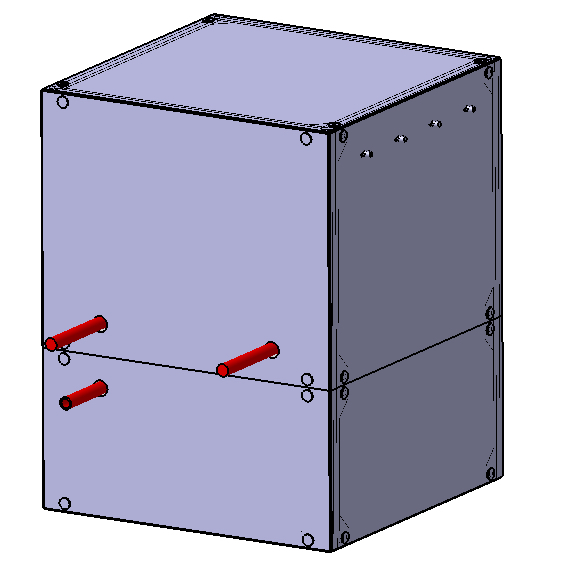
\includegraphics[width=0.7\textwidth]{4-experiment-design/img/frontal_holes.jpg}
%DIFDELCMD <     %%%
%DIFDELCMD < \caption{%
{%DIFAUXCMD
\DIFdelFL{.}}
    %DIFAUXCMD
%DIFDELCMD < \label{front_wall_holes}
%DIFDELCMD < \end{figure}
%DIFDELCMD < %%%
\DIFdelend %DIF > \begin{figure}[!ht]
%DIF >     \centering
%DIF >     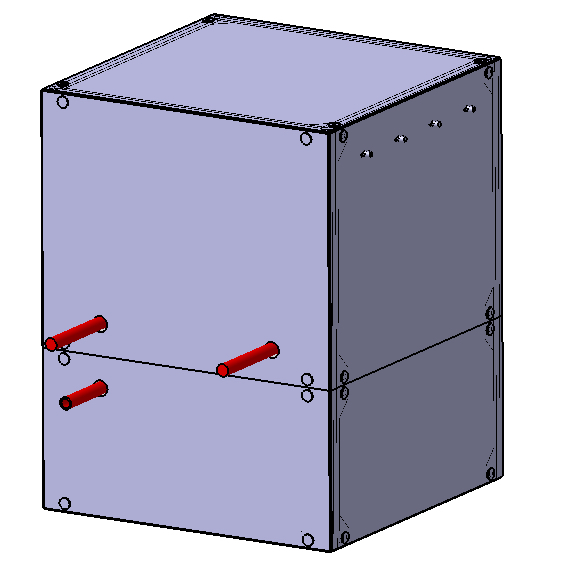
\includegraphics[width=0.7\textwidth]{4-experiment-design/img/frontal_holes.jpg}
%DIF >     \caption{External view of the experiment.}
%DIF >     \label{front_wall_holes}
%DIF > \end{figure}


\DIFdelbegin %DIFDELCMD < \pagebreak
%DIFDELCMD < %%%
\DIFdelend \subsubsection{Fixing Interface}

The two experiment box subsystem structures will be joined together by four anchor points\DIFaddbegin \DIFadd{, in black in Figure \ref{overview}}\DIFaddend . On the front and back side, two flat plates with two bolts each will interface both structures. 

This method will allow for easy and fast recovery of the CAC box. 


%% Figure with the two boxes attached


\DIFdelbegin %DIFDELCMD < \pagebreak
%DIFDELCMD < %%%
\DIFdelend \subsubsection{Manipulation Interface}

The two-box system will be fixed to the gondola rails by using four 90-degree angles, 2 per rail. All the anchor points \DIFaddbegin \DIFadd{to the gondola }\DIFaddend will be in the AAC box since the CAC box will be already attached \DIFdelbegin \DIFdel{the itby four anchor points}\DIFdelend \DIFaddbegin \DIFadd{to it}\DIFaddend . The latter also ensures that the AAC box will remain properly fixed in the gondola after the CAC fast recovery. 

\smallskip
In order to access the experiment once fixed in the gondola, the walls could be removed when necessary providing access in all three directions. They can be screwed in again once the manipulation is done.


Several handles will be placed to allow an easy and safe manipulation of \DIFdelbegin \DIFdel{the experiment box in }\DIFdelend both the CAC and the AAC boxes. 


\subsubsection{Mechanical Components}

All the components used in the mechanical design can be found in Table \ref{tab:mechanical-components}. Spare elements are not included. 


\raggedbottom
\pagebreak
\subsection{Electrical Design}

\subsubsection{Block Diagrams}
\begin{centering}
The electronics design can be seen in Figure \ref{fig:electronics-block-diagram} and the interfaces this requires can be seen in Figure \ref{fig:eee-interface-diagram}. There will be four distinct areas, the Electronics box, the valve centre, the pump box and the CAC system. All connections to the outside of the box are located in the electronics box. These are the voltage regulators for the external power source and the Ethernet shield with an SD data storage which will connect to the Telemetry, Tracking, and Command (TT\&C). Additionally one pressure sensor, one heater and one temperature sensor will be placed in this area. The CAC system area will contain three temperature sensors to monitor its ambient temperature and one electronic valve to be closed before landing. In the AAC system area there will be eleven valves, one airflow sensor, one pressure sensor, five temperature and one humidity sensor and a heater. In the pump box there will be the miniature diaphragm air pump, one temperature sensor and one heater.
\end{centering}
\bigskip

\begin{figure}[H]
    \begin{align*}
        \DIFdelbeginFL %DIFDELCMD < 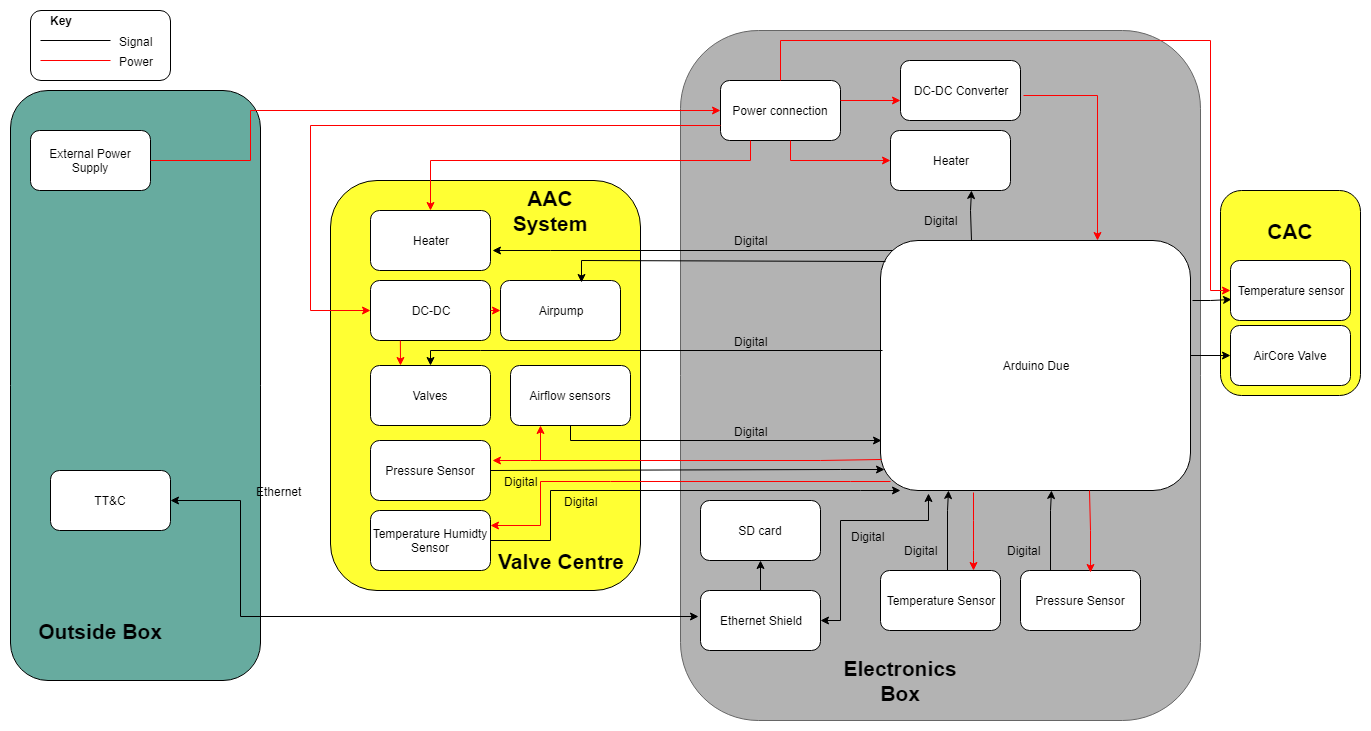
\includegraphics[width=16cm]{4-experiment-design/img/eee-block-diagram-march.png}
%DIFDELCMD <     %%%
\DIFdelendFL \DIFaddbeginFL 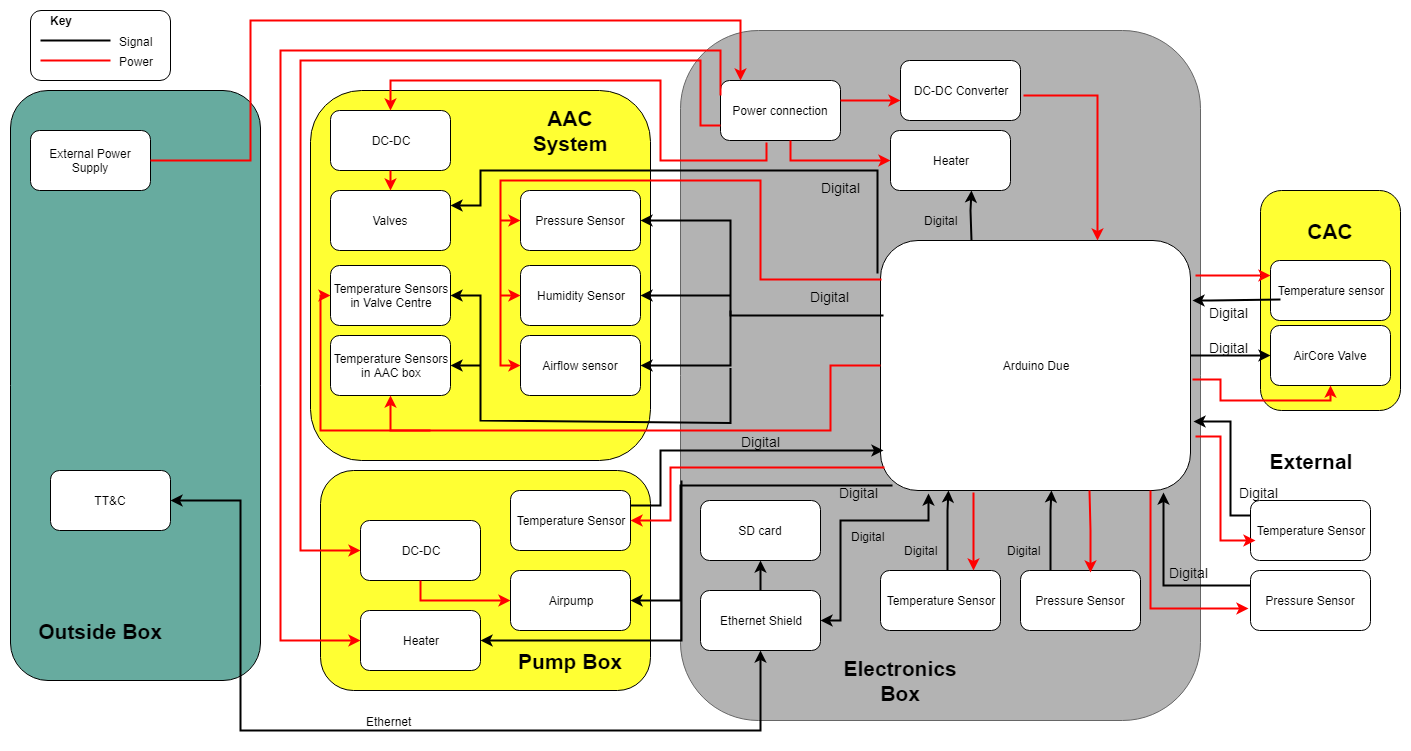
\includegraphics[width=16cm]{4-experiment-design/img/block-diagram-four-sections.png}
    \DIFaddendFL \end{align*}
    \caption{Block Diagram for all Electronic Components Showing the Signal and Power Connections}\label{fig:electronics-block-diagram}
\end{figure}


\begin{figure}[H]
    \begin{align*}
        \DIFdelbeginFL %DIFDELCMD < 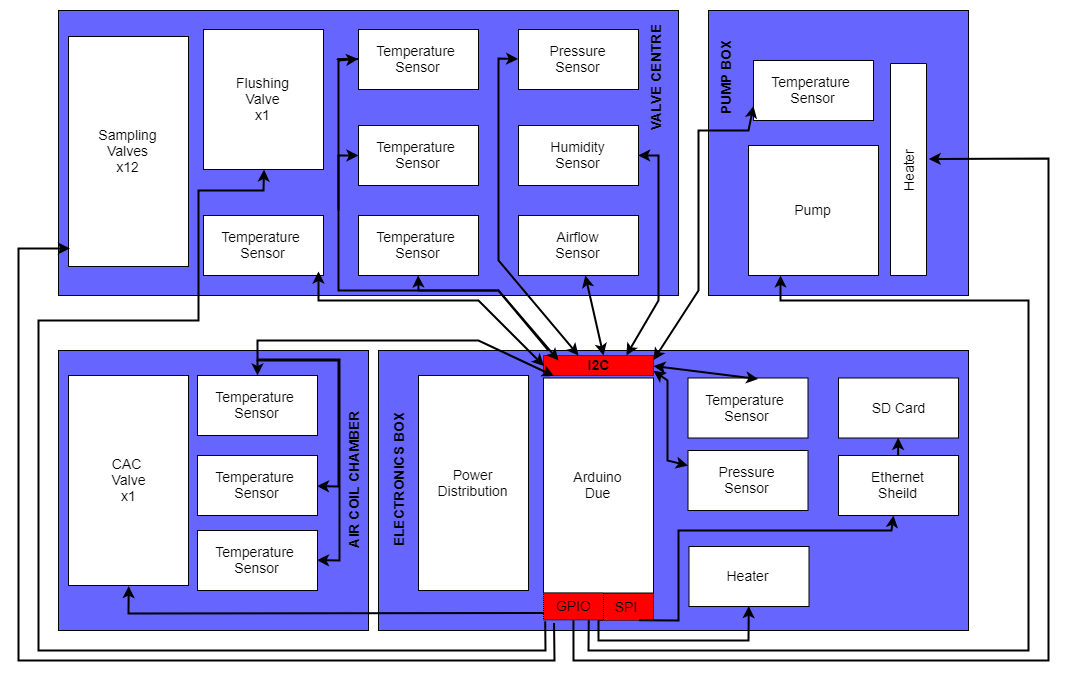
\includegraphics[width=16cm]{4-experiment-design/img/eee-interface-diagram.png}
%DIFDELCMD <     %%%
\DIFdelendFL \DIFaddbeginFL 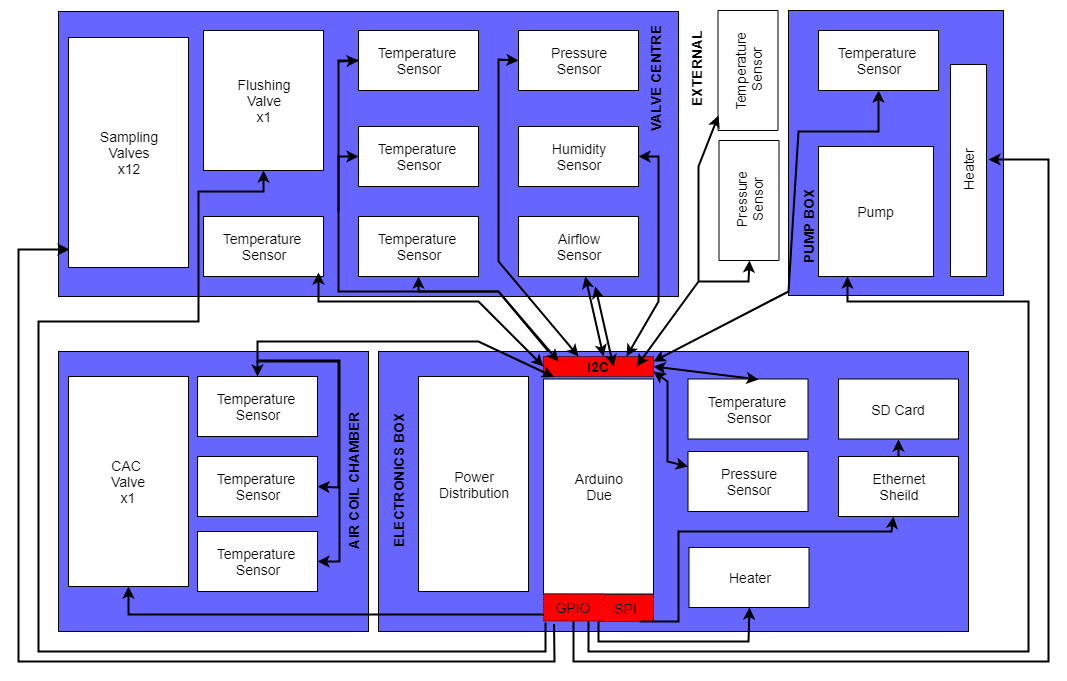
\includegraphics[width=16cm]{4-experiment-design/img/INTERFACE-DIAGRAM-2.png}
    \DIFaddendFL \end{align*}
    \caption{Block Diagram Showing the Interfaces Between All Electrical Components.}\label{fig:eee-interface-diagram}
\end{figure}

\begin{centering}
Three DC-DC converters will be used to step down the voltage from the 28.8V provided by the gondola down to: 
\end{centering}

\begin{centering}
\begin{itemize}
  \item $28.8V \Longrightarrow 12V$ for the Arduino.  
  \item $28.8V \Longrightarrow 24V$ for the valves.
  \item $28.8V \Longrightarrow 24V$ for the pump.
  \end{itemize}

\end{centering}
\bigskip

\begin{centering}
The heaters will not require the voltage to be stepped down and so will be powered directly from the gondola battery.
\end{centering}
\bigskip

\subsubsection{Miniature Diaphragm Pump}
\DIFdelbegin \DIFdel{PLACE HOLDER. INFORMATION AND PICTURE WILL BE PLACED HERE BEFORE MONDAY. }\DIFdelend \DIFaddbegin \DIFadd{The pump which has been selected is the KNF 850.1.2. KNDC B, Figure \ref{fig:pumppic}, which is manufactured by KNF. One of the reasons this pump has been selected is that it has successfully been flown on a similar flight in the past \mbox{%DIFAUXCMD
\cite{LISA}}\hspace{0pt}%DIFAUXCMD
. On this flight it managed to pump 180mL of air at 25km altitude. However, to ensure the pump will operate as intended several low pressure and low temperature tests will be completed.
}\DIFaddend 

\DIFdelbegin \subsubsection{\DIFdel{Solenoid Valves}}
%DIFAUXCMD
\addtocounter{subsubsection}{-1}%DIFAUXCMD
\DIFdel{PLACE HOLDER. INFORMATION AND PICTURE WILL BE PLACED HERE BEFORE MONDAY. }\DIFdelend \DIFaddbegin \DIFadd{The pump has a maximum flow rate of 8.0LPM when at ambient pressure. This is in excess of the required flow rate as the flow rate will decrease as the altitude increases. As the pressure decreases the current required by the pump will increase until it hits a peak current draw of 340mA. However as seen in Figure \ref{fig:pumpflowcur} the peak current then decreases as the pressure continues to decrease. It is also worth noting that whilst the flow rate appears to decrease too much Figure \ref{fig:pumpflowcur} is assuming that this is the pressure differential. Our bags will not be at vacuum and they will not be pressurized therefore the expected flow rate performance is higher.
}\DIFaddend 

\DIFaddbegin \begin{figure}[H]
    \begin{align*}
        \DIFaddFL{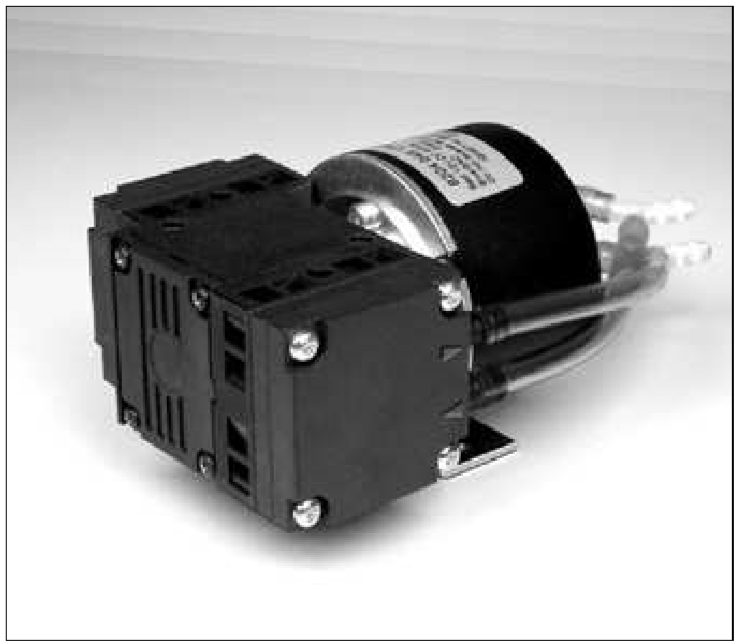
\includegraphics[width=6cm]{4-experiment-design/img/pump-850-1-2-kndc-b.png}
    }\end{align*}
    \caption{\DIFaddFL{KNF 850.1.2. KNDC B Miniature Diaphragm Pump}}\label{fig:pumppic}
\end{figure}


\begin{figure}[H]
    \begin{align*}
        \DIFaddFL{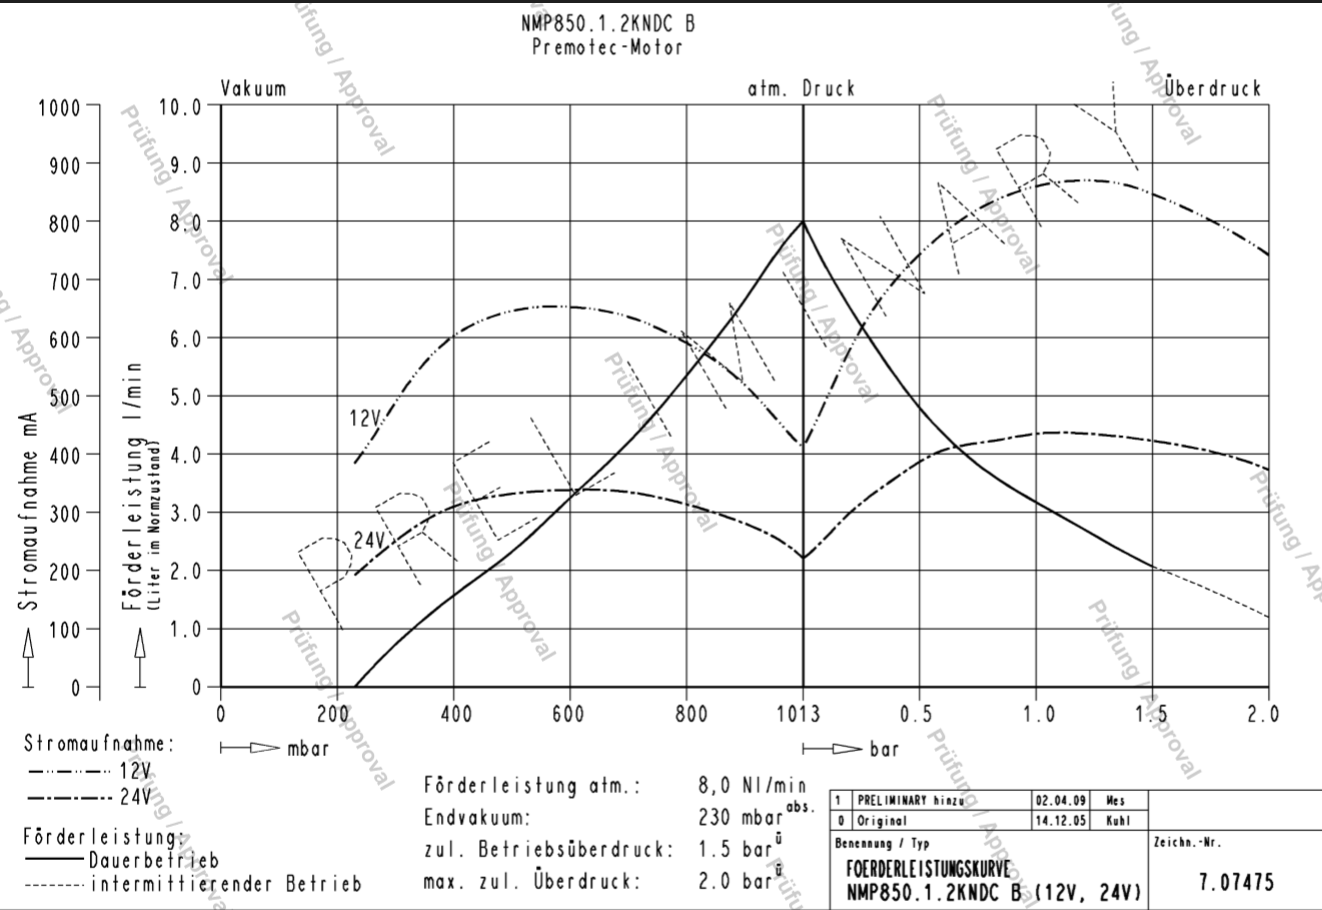
\includegraphics[width=15cm]{4-experiment-design/img/pump-flow-rate-current-graph.png}
    }\end{align*}
    \caption{\DIFaddFL{KNF 850.1.2. KNDC B Flow Rate and Current Draw to Pressure Graph.}}\label{fig:pumpflowcur}
\end{figure}


\subsubsection{\DIFadd{Electromagnetically Controlled Valves}}
\DIFadd{Filling of the air bags will be controlled by the solenoid valves. For this purpose Parker solenoid valve 121K63, Figure \ref{fig:valve},  with the 24 VDC coil, Figure \ref{fig:coil}, has been selected after careful consideration of the different options available in the market and keeping the experiment requirements in mind. The valves will be normally closed through out the experiment with zero power consumption and will be open, when given power, to fill up the air bags at specific altitudes or to flush the tubes.
}

\begin{figure}[H]
    \begin{align*}
        \DIFaddFL{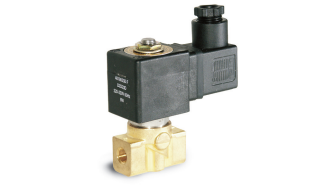
\includegraphics[width=6cm]{4-experiment-design/img/valve.png}
    }\end{align*}
    \caption{\DIFaddFL{Valve}}\label{fig:valve}
\end{figure}

\begin{figure}[H]
    \begin{align*}
        \DIFaddFL{\includegraphics[width=2cm]{4-experiment-design/img/Coil.png}
    }\end{align*}
    \caption{\DIFaddFL{Coil}}\label{fig:coil}
\end{figure}


\DIFadd{The port size of the valve is 1/4" which is compatible with the gas analyzer. The coil can withstand temperature from -40 to 50 °C which is suitable for flight operations at high altitudes. Although the valve can operate under a maximum pressure drop of 100 bar it also needs to be tested at intended low pressure values. For this purpose one valve with the motor and a shield, Figure \ref{fig:shield}, has already been ordered.  
}


\begin{figure}[H]
    \begin{align*}
        \DIFaddFL{\includegraphics[width=2cm]{4-experiment-design/img/Shield.png}
    }\end{align*}
    \caption{\DIFaddFL{Shield}}\label{fig:shield}
\end{figure}

\newpage
\DIFaddend \subsubsection{Valve Driving Circuit}
\DIFdelbegin \DIFdel{PLACE HOLDER. CIRCUIT DIAGRAM AND EXPLANATION WILL BE PLACED HERE BEFORE MONDAY. }\DIFdelend \DIFaddbegin \DIFadd{The valves will be powered through a 50W DC-DC converter that will step down the 28.8V to 24V. They will also have a connection to the Arduino so that they can be controlled. In order to allow this connection a switching circuit has been devised using a power MOSFET and a BJT. This circuit is detailed in Figure \ref{fig:switchcir}.
}\DIFaddend 

\DIFaddbegin \begin{figure}[H]
    \begin{align*}
        \DIFaddFL{\includegraphics[width=8cm]{4-experiment-design/img/switching-circuit-2.png}
    }\end{align*}
    \caption{\DIFaddFL{Schematic showing the switching circuit to drive the valves through the Arduino}}\label{fig:switchcir}
\end{figure}

\DIFadd{The power MOSFET will control the valves ON-OFF state whilst the BJT will connect directly to the Arduino and ensure that the valve is only turned on when a true signal is given. The power MOSFET will be on when the BJT is on. The BJT will be on when a signal of 3.3V is given and off when a signal of 0V is given. Three resistors will also be used. The purpose of \mbox{%DIFAUXCMD
$R_{1}$
}%DIFAUXCMD
is to protect the Arudino and also to step up the current entering the BJT. The value has been chosen to ensure that enough current reaches the valve to turn it on. \mbox{%DIFAUXCMD
$R_{2}$
}%DIFAUXCMD
is an optional resistor which creates a voltage divider that further increases the current entering the BJT. Finally \mbox{%DIFAUXCMD
$R_{3}$
}%DIFAUXCMD
is for when the BJT is off to avoid creating a short circuit. 
}


\DIFaddend \raggedbottom
\pagebreak
\subsection{Thermal Design} \label{Thermal_section}

\DIFaddbegin \subsubsection{\DIFadd{Thermal Environment}}
\DIFaddend \begin{centering}
The experiment will experience a wide range of temperatures during the flight and it must be able to continue to operate despite these changes. As seen in Figure \ref{fig:temperature-profile} the coldest point of the flight will be between 15km and 20km where the air temperature can drop to $-80\degree$C and temperatures on the gondola have been recorded as low as $-40\degree$C during the float phase in the past \cite{BexusManual}. In addition launching from Kiruna in late October means the temperature on the ground could be as low as $-15\degree$C. As our lowest operating temperature component must be at a minimum of $0\degree$C this could mean heaters may need to be switched on while the experiment is still on the ground. 
\end{centering}


\begin{figure}[H]
    \begin{align*}
        \includegraphics[height=5cm]{4-experiment-design/img/temperature-profile.png}
    \end{align*}
    \caption{Diagram showing the temperature profile of the atmosphere \cite{jacob}}\label{fig:temperature-profile}
\end{figure}

\DIFaddbegin \subsubsection{\DIFadd{Overall Design}}
\DIFaddend \begin{centering}
To protect the components against the cold two heaters will be included. One of these will be placed close to the Arduino, which is anticipated to be able to keep the controller area warm enough, and the second will be placed close to the valves to ensure they continue to operate as expected. To control these heaters two temperature sensors will also be onboard in similar locations. If the reading from one of the temperature sensors is lower than the predefined value then the heater will turn on. 
\DIFdelbegin \DIFdel{The predefined value will be chosen based upon the minimum operating temperature of the components. It is also expected that the electrical components will produce some heat themselves.
}\DIFdelend \end{centering}


\begin{centering}
In addition to using electrical heaters the experiment will also be thermally insulated. The Styrofoam casing which will be used to protect the CAC from impact forces will also serve as insulation. It is also planned to add additional insulation around the components.  
\end{centering}

\begin{centering}
It is also important to consider heating from the sun which could raise the temperature of the experiment considerably. Sufficient insulation should be included to ensure the inside of the box stays within the operating temperature range. This will be investigated at a later date when a full CFD thermal analysis is completed.
\end{centering}
\bigskip

\pagebreak

\begin{longtable}{|m{1cm}|m{3.5cm}|m{1cm}|m{1cm}|m{1cm}|m{1cm}|}
\hline
\multirow{2}{*}{\textbf{ID}} & \multirow{2}{*}{\textbf{Components}}                                 & \multicolumn{2}{l|}{\textbf{Operating T (°C)}} & \multicolumn{2}{l|}{\textbf{Survivable (°C)}} \\ \cline{3-6} 
                             &                                                                      & Min.                   & Max.                  & Min.                  & Max.                  \\ \hline
1                            & Arduino Due                                                          & -40                    & 85                    & -60                   & 150                   \\ \hline
2                            & Arduino Ethernet Shield 2                                            & -40                    & 85                    & -65                   & 150                   \\ \hline
3                           & \DIFaddbegin \DIFadd{KNF   850.1.2.KNDC   BMiniature Diaphragm Pump                                                            }& \DIFadd{5                      }& \DIFadd{50                      }& \DIFadd{-20                    }& \DIFadd{100                      }\\ \hline
\DIFadd{4                            }& \DIFaddend Barometric Pressure Sensor MS5607-02BA03                             & -40                    & 85                    & -40                   & 125                   \\ \hline
\DIFdelbegin \DIFdel{4                            }\DIFdelend \DIFaddbegin \DIFadd{5                          }\DIFaddend & \DIFaddbegin \DIFadd{Electromagnetically controlled valve                                 }&  \DIFadd{-40                      }& \DIFadd{50              }& \DIFadd{-40                      }& \DIFadd{50                      }\\ \hline
\DIFadd{6                            }& \DIFaddend Airflow sensor AWM40000 Series                                       & -40                    & 125                   & -40                   & 125                   \\ \hline
\DIFdelbegin \DIFdel{5                            }\DIFdelend \DIFaddbegin \DIFadd{9                            }\DIFaddend & Temperature sensor VSSOP-8, LM70, LM70CIMM-5/NOPB & -55                    & 150                   & -65                   & 150                   \\ \hline
\DIFdelbegin \DIFdel{6                           }\DIFdelend \DIFaddbegin \DIFadd{10                            }\DIFaddend & \DIFaddbegin \DIFadd{DC-DC step converter                                                 }& \DIFadd{-40                       }& \DIFadd{85                       }& \DIFadd{-50                      }& \DIFadd{125                      }\\ \hline
\DIFadd{11                           }& \DIFaddend HDC2010 Low Power Humidity Digital Sensors                           & -40                    & 85                    & -40                   & 125                   \\ \hline
\DIFdelbegin \DIFdel{7                            }\DIFdelend \DIFaddbegin \DIFadd{12                           }\DIFaddend & Industrial temperature microSD XCUHS-I 8GB                           & -40                    & 85                    & -40                   & 85                    \\ \hline
\DIFdelbegin \DIFdel{8                            }%DIFDELCMD < & %%%
\DIFdel{DC-DC step converter                                                 }%DIFDELCMD < & %%%
\DIFdel{-40                       }%DIFDELCMD < & %%%
\DIFdel{85                       }%DIFDELCMD < & %%%
\DIFdel{-50                      }%DIFDELCMD < & %%%
\DIFdel{125                      }%DIFDELCMD < \\ \hline
%DIFDELCMD < %%%
\DIFdel{9                           }%DIFDELCMD < & %%%
\DIFdel{Electromagnetically controlled valve                                 }%DIFDELCMD < &  %%%
\DIFdel{-43                      }%DIFDELCMD < & %%%
\DIFdel{85              }%DIFDELCMD < & %%%
\DIFdel{-43                      }%DIFDELCMD < & %%%
\DIFdel{100                      }%DIFDELCMD < \\ \hline
%DIFDELCMD < %%%
\DIFdel{10                           }%DIFDELCMD < & %%%
\DIFdel{BTC Series PMDC Iron Core Brush Miniature Diaphragm Pump H084-11                                                            }%DIFDELCMD < & %%%
\DIFdel{5                      }%DIFDELCMD < & %%%
\DIFdel{50                      }%DIFDELCMD < & %%%
\DIFdel{-20                    }%DIFDELCMD < & %%%
\DIFdel{100                      }%DIFDELCMD < \\ \hline
%DIFDELCMD < %%%
\DIFdelend 


\caption{Thermal Table}
\label{tab:thermal-table}
\end{longtable}
\raggedbottom

\raggedbottom

\subsubsection{Internal Temperature}

As the current experiment model stands, an enclosed partition has been reserved in the lower front-right corner of the AAC section of the TUBULAR experiment. This partition will house all of the electronic components not required to be situated in specified locations throughout the experiment setting, \DIFdelbegin \DIFdel{as well as the pump and valves. 
The partition will }\DIFdelend \DIFaddbegin \DIFadd{such as some of the sensors. 
}

\DIFadd{Inside this partition will be three separate insulated boxes. The first of these is the Electronics box which will }\DIFaddend occupy a space measuring 20 cm in length, 10 cm in width, and 20 cm in height, and will be insulated from inside to outside with polyethylene, polystyrene, and finally aluminum. The infrastructure within this enclosure shall be such that the electronics are fitted together to in turn be bound within another box of insulated material (likely made from PVC)\DIFdelbegin \DIFdel{and will be appropriately labeled the "Electronics Box." Subsequently, above the electronics box}\DIFdelend \DIFaddbegin \DIFadd{. 
}

\DIFadd{Above the electronics box will be the second internal box, the pump box, where the pump }\DIFaddend will be situated \DIFdelbegin \DIFdel{the pump and the collection of valves - the valves being }\DIFdelend \DIFaddbegin \DIFadd{and the third internal box, the valve centre, where the valves will be situated. The valves will be }\DIFaddend routed together by several tubes to form a compact structure \DIFdelbegin \DIFdel{with the label "Valve Center" ascribed to it. 
As previously mentioned regarding the heaters, one }\DIFdelend \DIFaddbegin \DIFadd{aiding the thermal control over this area. 
}

\DIFadd{One heater }\DIFaddend will be included in the electronics box with its main priority being keeping the Arduino Due board within operational temperatures \DIFdelbegin \DIFdel{, and }\DIFdelend \DIFaddbegin \DIFadd{whilst }\DIFaddend delivering the remaining heat to peripheral electronics. The other heater will be fitted between the \DIFdelbegin \DIFdel{diaphragm of the }\DIFdelend pump and the entrances to the valve center and will \DIFdelbegin \DIFdel{carry the task of keeping }\DIFdelend \DIFaddbegin \DIFadd{keep }\DIFaddend its lateral neighbors within their respective \DIFdelbegin \DIFdel{functional }\DIFdelend \DIFaddbegin \DIFadd{operational }\DIFaddend temperature ranges.

The pump has the most critical temperature range \DIFdelbegin \DIFdel{in that }\DIFdelend \DIFaddbegin \DIFadd{as }\DIFaddend it is the only component that cannot operate below freezing temperatures\DIFdelbegin \DIFdel{- in fact, }\DIFdelend \DIFaddbegin \DIFadd{. It's data sheet states }\DIFaddend it must always be no colder than $5\degree$C, or the EPDM diaphragm \DIFdelbegin \DIFdel{will }\DIFdelend \DIFaddbegin \DIFadd{may }\DIFaddend not be able to expand and contract sufficiently to maintain the desired airflow of 8L/min. \DIFaddbegin \DIFadd{However as this pump has been used successfully on flights before, \mbox{%DIFAUXCMD
\cite{LISA}}\hspace{0pt}%DIFAUXCMD
, tests will be conducted on the pump to find its true performance at lower temperatures. }\DIFaddend The valves are also crucial to the experiment's function, as \DIFdelbegin \DIFdel{their correct function is }\DIFdelend \DIFaddbegin \DIFadd{they are }\DIFaddend what enables each and every sampling bag onboard to be used. For this reason, while the valves can operate down to $-43\degree$C, \DIFdelbegin \DIFdel{they still need to be kept }\DIFdelend \DIFaddbegin \DIFadd{it is desirable to be keep them }\DIFaddend above this limit whenever in use.

Given the thermal conductivity of EPDM ($0.2 W/(m.K)$), the \DIFaddbegin \DIFadd{pump's }\DIFaddend diaphragm experiences a minimal temperature drop across itself when one side is subject to the heater's temperature while the other end of the pump is leveled with the ambient temperature. \DIFdelbegin \DIFdel{Case in point, }\DIFdelend \DIFaddbegin \DIFadd{Through calculation }\DIFaddend it was found that at an ambient temperature of $-50\degree$C and a heater temperature at $10\degree$C, that the center of the pump\DIFdelbegin \DIFdel{- }\DIFdelend \DIFaddbegin \DIFadd{, }\DIFaddend the far end of the diaphragm\DIFdelbegin \DIFdel{- }\DIFdelend \DIFaddbegin \DIFadd{, }\DIFaddend measured $9.35\degree$C. Reassessing the equation yielded the most energy-conserving temperature that would keep the pump's diaphragm above the minimum requirement to be $7\degree$C\DIFdelbegin \DIFdel{- and this }\DIFdelend \DIFaddbegin \DIFadd{. This }\DIFaddend held whether the temperature \DIFdelbegin \DIFdel{were }\DIFdelend \DIFaddbegin \DIFadd{was }\DIFaddend as it could be on ground level ($-10\degree$C), or in floating phase ($-50\degree$C).

 \DIFaddbegin \begin{align*}
     \DIFadd{T_{inlet} }&\DIFadd{= 263 K}\\
    \DIFadd{T_{heated} }&\DIFadd{= 283 K}\\
    \DIFadd{L_{inlet} }&\DIFadd{= 0.038 m}\\
    \DIFadd{L_{phragm} }&\DIFadd{= 0.038 m}\\
    \DIFadd{k_{PPS} }&\DIFadd{= 2\frac{W}{m*K}}\\
    \DIFadd{k_{EPDM} }&\DIFadd{= 0.2\frac{W}{m*K}}\\
    \DIFadd{k_{air} }&\DIFadd{= 0.024\frac{W}{m*K}}\\
    \DIFadd{k_{phragm} }&\DIFadd{=  \frac{k_{EPDM}+4k_{air}}{5} = 0.06\frac{W}{m*K}}\\
    \DIFadd{T_{med} }&\DIFadd{= \frac{ k_{phragm}  L_{inlet} T_{inlet} + k_{PPS} L_{phragm} T_{heated} }{ k_{phragm} L_{inlet} + k_{PPS}  L_{phragm}} }\\
    \DIFadd{T_{med} }&\DIFadd{= \frac{ 0.06 (0.038)(263) + 2(0.038)(283)}{(0.06)(0.038) + (2)(0.038)} }\\
    \DIFadd{T_{med} }&\DIFadd{= 282.35 K \longrightarrow 9.35\degree C
 }\end{align*}

\DIFadd{Reworking the equation to fit the inlet face at the true ambient temperature of -50\mbox{%DIFAUXCMD
$\degree$
}%DIFAUXCMD
C and the reduced heater temperature of 7\mbox{%DIFAUXCMD
$\degree$
}%DIFAUXCMD
C gives the following:
}

%DIF >  nice :) Also remove the * and it will number the equations. Also also to start a new line just write \\ at the end and it will make the next thing appear on a new line. Also also also using &= aligns all the equals signs and makes it look nice :D I leave these tips here so delete when you don't need them :)



 \begin{align*}
     \DIFadd{T_{inlet} = 223 K}\\
    \DIFadd{T_{heated} = 280 K}\\
    \DIFadd{T_{med} = \frac{ k_{phragm} L_{inlet} T_{inlet} + k_{PPS} L_{phragm} T_{heated} }{ k_{phragm} L_{inlet} + k_{PPS}  L_{phragm}}}\\
    \DIFadd{T_{med} = \frac{ 0.06 (0.038)(223) + 2(0.038)(280)}{(0.06)(0.038) + (2)(0.038)}}\\
    \DIFadd{T_{med} = 278.28 K \longrightarrow 5.28\degree C
 }\end{align*}

\DIFaddend \subsubsection{Box Analysis}
\DIFaddbegin 

\DIFadd{For the box temperature to be properly estimated, the other two divisions within the component enclosure need to be taken into account. The manifold comprising the valve center is made of a compound of nylon (assumed to be nylon-6) and kynar. It has also been assumed they are used equally in mass and distribution at this stage of thermal estimation.
}

 \begin{align*}
    \DIFadd{T_{outlet} }&\DIFadd{= 263 K}\\
    \DIFadd{T_{heated} }&\DIFadd{= 283 K}\\
    \DIFadd{L_{outhalf}}& \DIFadd{= 0.038 m}\\
    \DIFadd{L_{inhalf} }&\DIFadd{= 0.038 m}\\
    \DIFadd{k_{Nylon-6} }&\DIFadd{= 0.24\frac{W}{m*K}}\\
    \DIFadd{k_{Kynar} }&\DIFadd{= 0.162\frac{W}{m*K}}\\
    \DIFadd{k_{manifold} }&\DIFadd{=  \frac{k_{Nylon-6}+k_{Kynar}}{2} = 0.201\frac{W}{m*K}}\\
    \DIFadd{T_{med} }&\DIFadd{= \frac{ k_{manifold} L_{inhalf} T_{heated} + k_{manifold} L_{outhalf} T_{outlet} }{ k_{manifold} L_{inhalf} + k_{manifold}  L_{outhalf}}}\\
    \DIFadd{T_{med} }&\DIFadd{= \frac{ 0.201 (0.040)(223) + 0.201(0.040)(280)}{(0.201)(0.040) + (0.201)(0.040)}}\\ 
    \DIFadd{T_{med} }&\DIFadd{= 251.59 K or -21.41\degree C
 }\end{align*}
\DIFaddend \pagebreak
\subsection{Power Design}

\subsubsection{Power System Requirements}
\begin{centering}
The Gondola provides 28.8 V \DIFdelbegin \DIFdel{/1 mA }\DIFdelend or 13 Ah battery with a recommended maximum current draw of 1.8A \cite{BexusManual}. The experiment must run on external power from 4 hours before launch during the countdown phase and for the entire flight duration, lasting approximately 4 hours. As a factor of safety the experiment should be able to run for an additional 2 hours. 
\end{centering}

\begin{longtable}{|m{0.03\textwidth}| m{0.3\textwidth} |m{0.14\textwidth} |m{0.16\textwidth}|m{0.13\textwidth}| m{0.14\textwidth} |}
\hline
\textbf{ID}             & \textbf{Component}                                                   & \textbf{Voltage {[}V{]}} & \textbf{Current {[}mA{]}} & \textbf{Power {[}W{]}} & \textbf{Total {[}Wh{]}} \\ \hline
1                       & Arduino Due                                       & 12                                          & 30                                           & 0.36                                      & 36                                         \\ \hline
\DIFdelbegin \DIFdel{2                       }\DIFdelend \DIFaddbegin \DIFadd{3                       }\DIFaddend & \DIFdelbegin \DIFdel{BTC Series PMDC Iron Core Brush Miniature Diaphragm Pump                         H084-11                         }\DIFdelend \DIFaddbegin \DIFadd{KNF   850.1.2.KNDC   BMiniature Diaphragm Pump                         }\DIFaddend & 24                                          & \DIFdelbegin \DIFdel{180                                         }\DIFdelend \DIFaddbegin \DIFadd{320                                         }\DIFaddend & \DIFdelbegin \DIFdel{4.32                                      }\DIFdelend \DIFaddbegin \DIFadd{7.68                                      }\DIFaddend & \DIFdelbegin \DIFdel{4.32                                       }\DIFdelend \DIFaddbegin \DIFadd{7.68                                       }\DIFaddend \\ \hline
\DIFdelbegin \DIFdel{3                       }\DIFdelend \DIFaddbegin \DIFadd{4                       }\DIFaddend & Barometric Pressure Sensor MS5607-02BA03          & 3.3                                         & 1.4                                          & 0.00462                                   & 0.1                                        \\ \hline
\DIFdelbegin \DIFdel{4                       }\DIFdelend \DIFaddbegin \DIFadd{5                       }\DIFaddend & Electromagnetically controlled valve              & 24                                          & 458                                          & 11                                        & 75                                         \\ \hline
\DIFdelbegin \DIFdel{5                       }\DIFdelend \DIFaddbegin \DIFadd{6                       }\DIFaddend & Airflow sensor AWM40000 Series                    & 10                                          & 6                                            & 0.060                                     & 0.6                                        \\ \hline
\DIFdelbegin \DIFdel{6                       }\DIFdelend \DIFaddbegin \DIFadd{7                       }\DIFaddend & Polyimide Thermofoil Heaters HK5161R78.4L12       & 28                                          & 357                                          & 10                                        & 100                                        \\ \hline
\DIFdelbegin \DIFdel{7                       }\DIFdelend \DIFaddbegin \DIFadd{8                       }\DIFaddend & Polyimide Thermofoil Heaters HK5160R157L12        & 28                                          & 179                                          & 5                                         & 50                                         \\ \hline
\DIFdelbegin \DIFdel{8                       }\DIFdelend \DIFaddbegin \DIFadd{9                       }\DIFaddend & Temperature sensor VSSOP-8, LM70, LM70CIMM-5/NOPB & 5.5                                         & 0.49                                         & 0.002695                                  & 0.054                                      \\ \hline
\DIFdelbegin \DIFdel{9                       }\DIFdelend \DIFaddbegin \DIFadd{10                       }\DIFaddend & DC-DC step converter                              & 28                                          & 500 (output)                                 & 0.09                                      & 0.9                                        \\ \hline
\DIFdelbegin \DIFdel{10                      }\DIFdelend \DIFaddbegin \DIFadd{11                      }\DIFaddend & HDC2010 Low Power Humidity Digital Sensors        & 3.3                                         & 0.0005                                       & 1.65$\times10^{-6}$                              & 16.5$\times10^{-6}$                               \\ \hline
\multicolumn{1}{|c|}{-} & \textbf{Total}                                  & \multicolumn{1}{c|}{-}                      & \DIFdelbegin %DIFDELCMD < \multicolumn{1}{c|}{1671}                    %%%
\DIFdelend \DIFaddbegin \multicolumn{1}{c|}{1811}                    \DIFaddend & \DIFdelbegin %DIFDELCMD < \multicolumn{1}{c|}{41.42}                 %%%
\DIFdelend \DIFaddbegin \multicolumn{1}{c|}{44.77}                 \DIFaddend & \DIFdelbegin \DIFdel{267                                        }\DIFdelend \DIFaddbegin \DIFadd{270                                        }\DIFaddend \\ \hline
\multicolumn{1}{|c|}{-} & \textbf{Available from gondola}                 & \multicolumn{1}{c|}{-}                      & \multicolumn{1}{c|}{-}                       & \multicolumn{1}{c|}{-}                    & 374                                        \\ \hline

\caption{Power Design Table}
\label{tab:power-design-table}
\end{longtable}
\raggedbottom

%   $16.5\times10^{blah}$

\subsubsection{Power System Control and Regulation}
\DIFdelbegin \DIFdel{THIS IS A PLACEHOLDER. INFORMATION ON THE USE OF }\DIFdelend \DIFaddbegin \DIFadd{The power on board will be split using three }\DIFaddend DC-DC \DIFdelbegin \DIFdel{CONVERTERS WILL BE PLACED HERE BEFORE MONDAY. }\DIFdelend \DIFaddbegin \DIFadd{converters. Due to the relatively high loading that will be placed on the DC-DC converter by the valves it was decided to use two DC-DC converters to step down from 28.8V to 24V giving the pump its own dedicated DC-DC converter. This is as the pump and valves both have a high peak current draw. The Arduino will also have its own DC-DC converter stepping the voltage down from 28.8V to 12V. It is thought using three DC-DC converters will provide the best compromise between efficiency, cost and heating.
}\DIFaddend 

\raggedbottom

\pagebreak
\subsection{Software Design}
\subsubsection{Purpose}
The purpose of the software is to automatically control the valves so that they will be opened/closed at the designated altitude. Moreover, the software will store housekeeping data from sensors, pump and valves states to the on-board memory storage device. To determine a vertical profile, the acquisition of sensor data is required. From Olivier's research:
\begin{quote}
"In order to determine the vertical profiles of CO$_2$ and CH$_4$ from the analysis of sampled air, measurements of several atmospheric parameters are needed (see Sect. 2.3). The two most important parameters are the ambient pressure and the mean coil temperature. Those parameters are recorded by the AirCore-HR electronic data package. Mean coil temperature is obtained by taking the mean of three temperatures recorded by independent probes located at different positions along the AirCore-HR".\cite{Olivier}
\end{quote}
The next purpose is to transmit such data to the ground. It will allow the team to monitor the real-time condition of the experiment. Telecommand is also needed to take over the experiment if the software automation fails, since this experiment is highly dependent on the software. It will also be used to test the system, especially valves and heaters.\par
\subsubsection{Design}
\begin{enumerate}[label=(\alph*)]
\item{Process Overview}\\
The software which run on Arduino Due reads from the sensors through the I2C interface. The sensors provides temperature, pressure, airflow and humidity data. The acquired data will be time-stamped and stored on the on-board SDcard and transmitted via the E-Link System to the ground station. Then according to the pressure/altitude, the software controls the valves which will allow the air to flow inside the tube and bags. Figure \ref{processOverview} visually explain the process flow.
\begin{figure}[H]
    \centering
    \includegraphics[width=0.85\textwidth]{4-experiment-design/img/Process-overview-V0-1.png}
    \caption{The process overview of the experiment}
    \label{processOverview}
\end{figure}
\item{General and Safety related concepts}\\
Watchdog timer, which is an electronic countdown timer that causes an interrupt when it reaches 0, will be used to avoid failure because of a freezing software. During normal operations, the software will regularly reset the the watchdog timer to prevent it from elapsing, or \enquote{timing out}. Telecommands will also be used as backup in case the automation fails or otherwise become unresponsive. Telemetry will be utilized to transmit housekeeping data and the state of the valves to get conformation of operation. Rigorous testing will be performed during the development of the project and before the launch phase to insure that that the software is capable to control the experiment.\\
\\
Watchdog has been suggested to be removed in Preliminary Design Review. However, it is still a good feature for automatic reset in case the software freeze/stuck. Therefore, the watchdog will be kept and shall be tested before Critical Design Review.
\item{Interfaces}\\
Table \ref{tab:comIntpro} demonstrates how the components will interact with the onboard computer (OBC). Components that use SPI, will share MISO, MOSI, and CLK pins on the Arduino board. Each of them will also be connected to general pins input output (GPIO) for slave select. Furthermore, components using I2C protocol, will share Serial Data pin (SDA) and Serial Clock pin (SCL).

\begin{table}[H]
\centering
\begin{tabular}{lll}
Components interacting & Communication protocol & Interface                 \\ \hline
Pressure Sensors-OBC   & I2C                    & Arduino I2C \\
Temperature sensors-OBC        & I2C                    & Arduino I2C \\
Airflow sensor-OBC     & I2C                    & Arduino I2C \\
Heaters-OBC            & Digital                & GPIO pins \\
Air pump-OBC           & Digital                & GPIO pins \\
Valve-OBC              & Digital                & GPIO pins                 \\
OBC-microSD Storage    & SPI                    & Arduino Ethernet shield   \\
OBC - E-Link           & Ethernet               & Ethernet port            
\end{tabular}%Tabular dude
\caption{Communication and interface protocols}
\label{tab:comIntpro}
\end{table}

Every transmission to/from the ground will utilize the E-link connection. The data packet which will be used is Ethernet Packet with a header contains the address of destination, followed by the data, and at the end there is a frame check sequence (FCS). The up-linked data packet will have the same structure, with header followed by commands and ended with FCS.
\item{Data Acquisition and Storage}\\
Data will be stored on the SD memory card on the Arduino Ethernet Shield. It is estimated that for the entire flight, all the sensors will produce $650$ kilo bytes or $5.2$ mega bits of data. The sampling rates of the sensors are dependent on the modes (see Figure \ref{fig:modediag}). In standby mode, the sampling rate is $1$ per $10$ seconds, since this is not the essential part. The sampling rate is increased in the Normal Operation (ascent) mode to $1$ per seconds. Moreover, in the the descent phase of the experiment, the sampling rate will be increased significantly to $10$ per one second.\\
\\
The data will be collected and presented as a matrix, where the first column is the time frame, the following columns are the sensors data. After the sensors data, there will also be housekeeping data, that keeps track of the valves, and heaters states. However, the size of the housekeeping data is not expected to surpass 20 bits per sampling.\\
\\
Data will be continuously down-linked and the total telemetry size is 4.788 MB for 5 hours of flight.
\item{Process Flow}\\
The process flow can be explained with the mode diagram in figure \ref{fig:modediag}. The software will start with Standby Mode, in which the software will get samples from all sensors. When the software got reading of pressure changes (decrease), it will change to Normal - Ascent mode, where the software will empty the tube and bags by opening the valves. Then, at certain altitudes, air sampling will be conducted during ascending phase. During floating phase, there will be nothing conducted. The software will go to Normal - Descent mode when it sense when the pressure reduction is considerably big, where the software will sample the air by opening the valves for each bag in their designated altitude. The air sampling during descent phase will only be started after the gondola stabilize after cut-off. The software will know this by the reduction of pressure value readings. The experiment goes to SAFE mode about $500 \, m$ before the landing, where all the valves will be closed. 
\begin{figure}[H]
    \begin{align*}
        \includegraphics[width=1\linewidth]{4-experiment-design/img/state-diagram-V1-2.png}
    \end{align*}
    \caption{Process diagram for the modes}\label{fig:modediag}
\end{figure}
\item{Modularization and Pseudo Code}\\
\begin{figure}[H]
    \begin{align*}
        \includegraphics[width=1\linewidth]{4-experiment-design/img/sw_design.png}
    \end{align*}
    \caption{Onboard Software Design Tree}\label{fig:obtree}
\end{figure}
The software design is produced by using object oriented approach. The functionality of the experiment has been divided into several objects and their children. The design tree is shown in Figure \ref{fig:obtree}.\\
\\
The Telemetry object is responsible to format the sensor/housekeeping data, and to transmit it. MODE is responsible for controlling the four modes of software. INIT will initialize the necessary software programs. COMMANDS reads the telecommands and execute their commands. The AIR SAMPLING CONTROL object have the four children objects. The first child is responsible for controlling the pump. The second child contains the parameters for the valves and pump. The third child reads the data from the sensors, a fourth child is responsible for manipulating the valves.\\
\\
The SENSOR object have two children objects. One for sampling the sensors and another for recording and storing the housekeeping data. The HEATER object have three children objects. One for reading the temperature sensor data, another for deciding if the heaters should be turn on/off. And the third child for turning it on/off.\\ 
\\
Each of the objects interacts with each others fulfilling mutually exclusive interaction. It means that any shared variables can only be accessed by one object at time. This is important considering the program is be fully automatic and to prevent unnecessary data lost. The objects interface diagrams and their sequence diagrams can be found in Appendix \ref{sec:appB} and \ref{sec:appC}.
\end{enumerate}
%\begin{figure}[H]
%    \centering
%    \includegraphics[width=1\textwidth]{4-experiment-design/img/hood-diagram-v1-0.png}
%    \caption{Hierarchic Object-Oriented Design of the software}
%    \label{fig:hood}
%\end{figure}
\subsubsection{Implementation}
The C/C++ programming language is used when programming the platform. Software's as Arduino IDE will be used, other software will be used if necessary. A real-time operating system is under consideration and might be implemented if its use is found warranted. 


\raggedbottom
\pagebreak
\subsection{Ground Support Equipment}
One personal computer will be used to connect to the E-Link through the Ethernet port. A GUI will be created to display the sensors data and a feature to change the parameters in the experiment. The GUI for the ground station shall be with MATLAB programming language and IDE.\par
The data shall be recorded and stored on the computer. 
\begin{figure}[H]
    \centering
    \includegraphics[width=0.6\textwidth]{4-experiment-design/img/gc-software-V1-2.png}
    \caption{The ground control software design tree}
    \label{fig:gcModel}
\end{figure}
Figure \ref{fig:gcModel} shows the preliminary design of the ground station. The RXTX object is responsible for receiving and transmitting data over the provided Ethernet connection. The READ object takes the input received from the user, and the DISPLAY object takes data received from the RXTX object and show the data to the user through the GUI.


\raggedbottom
\raggedbottom
\pagebreak
\section{Experiment Verification and Testing}

\subsection{Verification Matrix}

The verification matrix is made following the standard of \textit{ECSS-E-10-02A}. \cite{ECSSSecretariat}

\textit{There are four established verification methods:}
\newline \textit{A - Verification by analysis or similarity}
\newline \textit{I - Verification by inspection}
\newline \textit{R - Verification by review-of-design}
%\newline \textit{S - Verification by similarity}
\newline \textit{T - Verification by testing}

Currently, no verification has yet transpired due to the hardware and software components potentially fitting the requirements still being sought and ordered and/or requested. As the project advances and the parts for each division arrive or are developed, the verification methods will be revised, and test numbers and status will be assigned.

\makeatletter
\renewcommand\@makefntext[1]{\leftskip=3em\hskip-1em\@makefnmark#1}
\makeatother

\begin{longtable}[]{|m{0.06\textwidth}| m{0.48\textwidth} |m{0.13\textwidth} |m{0.1\textwidth}|m{0.1\textwidth}|}

\hline
ID   & Written requirement                                                                                                                                                     & Verification & Test number & Status \\ \hline
F.1  & The experiment \textit{shall} collect air samples.                                                                                                                               &      T        &  2, 7           &        \\ \hline
F.2  & The experiment's CAC System \textit{shall} collect air samples during the descent phase.                                                                                         &      T        &  2, 7           &        \\ \hline
F.3  & The experiment's AAC System \textit{shall} collect air samples.                                                                                                                  &     T         &  1, 2, 7           &        \\ \hline
F.4  & The experiment's AAC System \textit{shall} be able to collect air samples during the ascent phase.                                                                               &     T         & 1, 2, 7     &        \\ \hline
F.5  & The experiment's AAC System \textit{shall} be able to collect air samples during the descent phase.                                                                              &      T        & 1, 2, 7    &        \\ \hline
F.6  & The altitude from which a sampling bag will start sampling \textit{shall} be programmable.                                                                                       &     A,T         &  10           &        \\ \hline
F.7  & The altitude from which a sampling bag will stop sampling \textit{shall} be programmable.                                                                                        &    A,T          & 10            &        \\ \hline
F.8  & The experiment \textit{shall} pump air into the AAC Sampling Bags.                                                                                                               &     T        & 1, 7            &        \\ \hline
F.9  & The experiment \textit{should} measure the air intake to the Sampling Bags.                                                                                                      &       T       & 2, 10            &        \\ \hline
F.10 & The experiment \textit{shall} measure the ambient pressure.                                                                                                                      &       T       & 2, 10            &        \\ \hline
F.11 & The experiment \textit{shall} measure the Electronics Box temperature.                                                                                                                   &       T       & 2, 10            &        \\ \hline
F.12 & The experiment \textit{shall} measure the ambient humidity.                                                                                                                      &      A        & 2, 10            &        \\ \hline
F.13 & The experiment \textit{shall} measure the temperature inside the AAC Valve Box.                                                                                                  &      T        & 2, 10            &        \\ \hline
F.14 & The experiment \textit{should} measure the humidity inside the AAC Valve Box.                                                                                                    &      A        & 2, 10            &        \\ \hline
F.15 & The experiment \textit{shall} measure the time.                                                                                                                                  &        A, T      & 2, 10            &        \\ \hline
F.16 & The experiment \textit{shall} accept telecommand instructions to programme AAC sampling altitudes for each sampling bag.                                                         &      T        & 10            &        \\ \hline
F.17 & The experiment \textit{shall} accept telecommand instructions to open designated valves.                                                                                         &      T        & 1, 10            &        \\ \hline
F.18 & The experiment \textit{shall} accept telecommand instructions to close designated valves.                                                                                        &      T        & 1, 10            &        \\ \hline
F.19 & The experiment \textit{may} accept telecommand instructions to change the sampling rate of the ambient pressure sensor.                                                          &     T         & 10            &        \\ \hline
F.20 & The experiment \textit{may} accept telecommand instructions to change the sampling rate of the Electronics Box temperature sensor.                                                       &      T        & 10            &        \\ \hline
F.21 & The experiment \textit{may} accept telecommand instructions to change the sampling rate of the AAC Valve Box temperature sensor.                                                 &      T        & 10            &        \\ \hline
F.22 & The experiment \textit{may} accept telecommand instructions to turn on the air pump.                                                                                             &      T        & 10            &        \\ \hline
F.23 & The experiment \textit{may} accept telecommand instructions to turn off the air pump.                                                                                            &       T       & 10            &        \\ \hline
F.24 & The experiment \textit{may} accept telecommand instructions to turn on the Valve Heater.                                                                                         &      T        & 10            &        \\ \hline
F.25 & The experiment \textit{may} accept telecommand instructions to turn off the Valve Heater.                                                                                        &      T        & 10            &        \\ \hline
F.26 & The experiment \textit{may} accept telecommand instructions to turn on the Electronics Box Heater.                                                                                    &      T        & 10            &        \\ \hline
F.27 & The experiment \textit{may} accept telecommand instructions to turn off the Electronics Box Heater.                                                                                   &      T        & 10            &        \\ \hline
P.1  & The telecommand data rate \textit{shall} not be over 10Kb/s.                                                                                                                          &        T      & 8, 10            &        \\ \hline
P.2  & \st{The default sampling rate of the ambient pressure sensor during Standby mode \textit{shall} be 0.1 Hz.}\footnote{Replaced by P.23\label{replaceSoftVeri}}                                                                       &      T        & 10            &        \\ \hline
P.3  & \st{The default sampling rate of the ambient pressure sensor during Normal operation-ascent mode \textit{shall} be 0.2 Hz.}\textsuperscript{\ref{replaceSoftVeri}}                                                           &      T        & 10            &        \\ \hline
P.4  & \st{The default sampling rate of the ambient pressure sensor during Normal operation-descent mode \textit{shall} be 10 Hz.}\textsuperscript{\ref{replaceSoftVeri}}                                                           &       T       & 10            &        \\ \hline
P.5  & \st{The default sampling rate of the AAC Valve Box temperature sensor \textit{shall} be 1 Hz.}\textsuperscript{\ref{replaceSoftVeri}}                                                                                        &      T        & 10            &        \\ \hline
P.6  &\st{ The programmable sampling rate of the ambient pressure sensor \textit{shall} not be lesser than 0.1 Hz.}\textsuperscript{\ref{replaceSoftVeri}}                                                                          &      T        & 10            &        \\ \hline
P.7  & \st{The programmable sampling rate of the ambient pressure sensor \textit{shall} not be greater than 100 Hz.}\textsuperscript{\ref{replaceSoftVeri}}                                                                         &       T       & 10            &        \\ \hline
P.8  & \st{The programmable sampling rate of the Electronics Box temperature sensor \textit{shall} not be lesser than 1Hz.}\textsuperscript{\ref{replaceSoftVeri}}                                                                          &       T       & 10            &        \\ \hline
P.9  & \st{The programmable sampling rate of the Electronics Box temperature sensor \textit{shall} not be greater than 7Hz. }\textsuperscript{\ref{replaceSoftVeri}}                                                                        &        T      & 10            &        \\ \hline
P.10 & \st{The programmable sampling rate of the AAC Valve Box temperature sensor \textit{shall} not be lesser than 1 Hz. }\textsuperscript{\ref{replaceSoftVeri}}                                                                  &        T      & 10            &        \\ \hline
P.11 & \st{The programmable sampling rate of the AAC Valve Box temperature sensor \textit{shall} not be greater than 7 Hz. }\textsuperscript{\ref{replaceSoftVeri}}                                                                 &        T      & 10            &        \\ \hline
P.12 & The accuracy of the ambient pressure measurements \textit{shall} be -1.5/+1.5 mbar for 25$\degree$.                                                                              &        T      & 5, 10           &        \\ \hline
P.13 & The accuracy of the ambient temperature measurements \textit{shall} be +3.5/-2$\degree$C(max) for condition of -55$\degree$C to 150$\degree$C.                                   &       T, I       & 5, 10            &        \\ \hline
P.14 & The accuracy of the ambient humidity measurements \textit{shall} be +-2 percent.                                                                                                         &       TBD\footnote{The other elements still need to be found either in the store or online. \label{fn:vm1}}        &  10           &        \\ \hline
P.15 & The accuracy of the AAC Valve Box temperature measurements \textit{shall} be +3.5/-2$\degree$C(max).                                                                                                &       TBD\textsuperscript{\ref{fn:vm1}}       & 5, 10            &        \\ \hline
P.16 & The air intake rate of the air pump \textit{shall} be 3L/min.                                                                                                                       &       TBD\textsuperscript{\ref{fn:vm1}}       & 7            &        \\ \hline
P.17 & The temperature of the Electronics Box \textit{shall} not go below 0$\degree$C.                                                                                                   &       T       & 5           &        \\ \hline
P.18 & The temperature of the Electronics Box \textit{shall} not exceed 25$\degree$C.                                                                                                    &       T       & 5            &        \\ \hline
P.19 & The temperature of the AAC Valve Box \textit{shall} not go below 0$\degree$C.                                                                                                    &       T       & 5            &        \\ \hline
P.20 & The temperature of the AAC Valve Box \textit{shall} not exceed 25$\degree$C.                                                                                                     &      T        & 5            &        \\
                                                 \hline
P.21 & The AAC air sampling \textit{shall} filter out all water molecules before filling the sampling bags.                                                                             &        T      & 7            &        \\ \hline
P.22 & The CAC air sampling \textit{shall} filter out all water molecules before filling the tube.                                                                                      &         T     & 7            &        \\ \hline

P.23 & The sampling rate shall be 2Hz.                                                                                    &         A,T     & 10            &        \\ \hline


D.1  & The experiment \textit{shall} operate in the temperature profile of the BEXUS vehicle flight and launch.                                                                         &       T       & 5            &        \\ \hline
D.2  & The experiment \textit{shall} operate in the vibration profile of the BEXUS vehicle flight and launch.                                                                           &       T       & 9            &        \\ \hline
D.3  & The experiment \textit{shall} not disturb or harm the launch vehicle.                                                                                                            &      T        & 7            &        \\ \hline
D.4  & The experiment's communication system \textit{shall} be compatible with the gondola's E-link system.                                                                             &      T        & 8            &        \\ \hline
D.5  & The experiment's power supply \textit{shall
} be compatible with the gondola's provided power.                                                                                    &      T        &  11           &        \\ \hline
D.6  & The experiment \textit{shall} not disturb other experiments on the gondola.                                                                                                      &       A,I       & 7            &        \\ \hline
D.7  & The total DC current draw \textit{should} be below 1.8 A.                                                                                                                        &      A        & 11            &        \\ \hline
D.8  & The total power consumption \textit{should} be below 374 Wh.                                                                                                                      &       A,T       & 11            &        \\ \hline
D.9  & The experiment \textit{shall} be able to operate in low pressure conditions (300mbar) up to 30 km altitude.                                                                                       &      I        &  4           &        \\ \hline
D.10 & The components of the experiment \textit{shall} operate within their temperature ranges.                                                                                         &       T       & 5            &        \\  \hline
D.11 & The OBC \textit{shall} be able to autonomously control the heaters.                                                                                                              &         T     & 10            &        \\ \hline
D.12 & The ground station GC \textit{shall} be able to display some of the received data.                                                                                               &      T        & 2, 10            &        \\ \hline
D.14 & The experiment \textit{shall} be able to survive and operate between -30\degree C and 60\degree C.                                                                               &      T        & 5            &        \\ \hline
D.15 & The external components that are directly exposed to the outside environment \textit{shall} be able to operate in -70\degree C.                                                  &    T          & 5            &        \\ \hline
D.16 & The watchdog \textit{should} be able to reset the system.                                                                                                                        &        T      & 10            &        \\ 
 \hline
D.17 & The experiment \textit{shall} be able to autonomously turn itself off just before landing.                                                                                       &        T      &  7, 10           &        \\ \hline
D.18 & The experiment box \textit{shall} be placed with at least one face exposed to the outside.                                                                                       &     I, A         & -            &        \\ \hline
O.1  & The TUBULAR Team \textit{shall} send telecommands from the ground station to the experiment before and during the flight.                                             &    T          & 8            &        \\ \hline
O.2  & The TUBULAR Team \textit{shall} receive telemetry from the experiment during the flight.                                                                              &    T          & 8            &        \\ \hline
O.3  & The experiment \textit{shall} change modes autonomously.                                                                                                              &        T      & 10            &        \\ \hline
O.4  & The heating mechanism \textit{shall} work autonomously.                                                                                                               &        T      & 10            &        \\ \hline
O.5  & The experiment \textit{shall} store data autonomously.                                                                                                                &       T       & 2, 10            &        \\ \hline
O.6  & The Air sampling control system \textit{shall} work autonomously.                                                                                                     &        T      & 10            &        \\ \hline
O.7  & The Air sampling control system \textit{shall} work autonomously.The valves in air sampling control system \textit{should} be controllable from the ground station. &      T        & 1, 10            &        \\ \hline
O.8  & The experiment \textit{should} be able to handle a timeout or drop in the network connection.                                                                         &    T          &  8           &        \\ \hline
O.9  & The heaters \textit{should} be controllable from the ground station.                                                                                                  &     T         &  8, 10           &        \\ \hline
O.10 & The watchdog\footnote{An electronic timer that is used to detect and recover from computer malfunctions} \textit{should} be able to reset the system.               &     T         & 10            &        \\ \hline
O.11 & The system \textit{should} be able to be reset with a command from the ground station.                                                                                &     T         & 8, 10            &        \\ \hline
O.12 & The experiment \textit{should} enter different modes with a telecommand from the ground station.                                                                      &      T        & 8, 10            &        \\ \hline
C.1  & Constraints specified in the BEXUS User Manual                                                                                                                          &       I       & -            &        \\ \hline
C.2  & The person-hours allocated to project implementation is limited by university related factors such as exams, assignments, and lectures.                                 &      I        & -            &        \\ \hline
C.3  & Budget limited to TBD.                                                                                                                                                  &      TBD\footnote{Total budget cannot be determined until mechanical component selection has been confirmed and outreach budget has been assigned.}        & -            &        \\ \hline

\caption{Verification Matrix}
\label{tab:var-mat}
\end{longtable}
\raggedbottom
\pagebreak
\subsection{Test Plan}

The planned tests are as follows:

\begin{enumerate}
    \item Valves test in Table \ref{tab:valves-test}.
    \item Data collection test in Table \ref{tab:data-coll-test}.
    \item Weight verification in Table \ref{tab:weight-test}.
    \item Low pressure test in Table \ref{tab:vacuum-test}.
    \item Thermal test in Table \ref{tab:thermal-test}.
    \item Experiment assembly and disassembly test in Table \ref{tab:assemble-test}.
    \item Bench test in Table \ref{tab:bench-test}.
    \item E-Link test in Table \ref{tab:e-link-test}.
    \item Vibration test in Table \ref{tab:vibration-test}.
    \item Software operation test in Table \ref{tab:software-op-test}.
    \item Power systems test in Table \DIFdelbegin \DIFdel{\ref{tab:power-test}}\DIFdelend \DIFaddbegin \DIFadd{\ref{tab:electronics-test}}\DIFaddend .
    \item Experiment removal test in Table \ref{tab:removal-test}.
    \DIFaddbegin \item \DIFadd{Ground station - OBC connection test in Table \ref{tab:software-connection-test}.
    }\item \DIFadd{Ground station - OBC parameters reprogram test in Table \ref{tab:software-reprogram-test}.
    }\item \DIFadd{Ground station invalid commands test in Table \ref{tab:software-invalidcommand-test}.
    }\item \DIFadd{Sampling test in Table \ref{tab:Sampling system-test}.
    }\item \DIFadd{Samples' condensation test in Table \ref{tab:samples-condensation-test}.
    }\item \DIFadd{Pump low pressure test \ref{tab:pump-low-pressure-test}.
    }\item \DIFadd{PCB operations test \ref{tab:pcb-test}
    }\item \DIFadd{Switching circuit testing and verification \ref{tab:switching-test}
}\DIFaddend \end{enumerate}

\renewcommand\thempfootnote{\arabic{mpfootnote}}

\begin{table}[H]
\centering
\begin{minipage}{\textwidth}
\begin{tabular}{|m{0.3\textwidth}| m{0.7\textwidth} |}
\hline
\textbf{Test Number} & 1 \\ \hline
\textbf{Test Type} & Calibration and Verification \\ \hline
\textbf{Test Facility} & Kiruna Space Campus laboratory \\ \hline
\textbf{Tested Item} & Valve system \\ \hline
\multirow{2}{*}{\textbf{\begin{tabular}[c]{@{}l@{}}Test Level/ Procedure \\ and Duration\footnote[12]{All test procedure and duration's are subject to change. \label{fn:testing}}\end{tabular}}} & Test procedure: Test valves work at different air pressures and temperatures. Check valves respond to commands as expected. Ensure valve series are properly connected and properly seal.\\ & Test duration: 2 hours \\ \hline
\textbf{Test Campaign Duration} & Recurrent test until and during the launch campaign \\ \hline
\textbf{Test Campaign Date} & April \\ \hline
\textbf{Test Completed} & NO \\ \hline
\end{tabular}
\caption{Test 1: Valves calibration and verification}
\label{tab:valves-test}
\end{minipage}
\end{table}
\raggedbottom

\begin{table}[H]
\centering

\begin{tabular}{|m{0.3\textwidth}| m{0.7\textwidth} |}
\hline
\textbf{Test Number} & 2 \\ \hline
\textbf{Test Type} & Software \\ \hline
\textbf{Test Facility} & Kiruna Space Campus laboratory \\ \hline
\textbf{Tested Item} & Arduino, sensors, valves and pump \\ \hline
\multirow{2}{*}{\textbf{\begin{tabular}[c]{@{}l@{}}Test Level/ Procedure \\ and Duration\textsuperscript{\ref{fn:testing}}\end{tabular}}} & Test procedure: Run software for full flight duration and ensure data collection proceeds as expected. Particularly watch for error handling and stack overflow. \\ & Test duration: 5 hours. Based on previous BEXUS flight duration's.\\ \hline
\textbf{Test Campaign Duration} & 2 days (1 day build-up, 1 day testing) \\ \hline
\textbf{Test Campaign Date} & June \\ \hline
\textbf{Test Completed} & NO \\ \hline
\end{tabular}
\caption{Test 2: Data collection test description}
\label{tab:data-coll-test}
\end{table}
\raggedbottom

\begin{table}[H]
\centering

\begin{tabular}{|m{0.3\textwidth}| m{0.7\textwidth} |}
\hline
\textbf{Test Number} & 3 \\ \hline
\textbf{Test Type} & Weight Verification \\ \hline
\textbf{Test Facility} & Kiruna Space Campus laboratory \\ \hline
\textbf{Tested Item} & The entire experiment \\ \hline
\multirow{2}{*}{\textbf{\begin{tabular}[c]{@{}l@{}}Test Level/ Procedure \\ and Duration\textsuperscript{\ref{fn:testing}}\end{tabular}}} & Test procedure: Use scales to measure the weight of the entire experiment. \\ & Test duration: 1 minute\\ \hline
\textbf{Test Campaign Duration} & 1 day \\ \hline
\textbf{Test Campaign Date} & July-August \\ \hline
\textbf{Test Completed} & NO \\ \hline
\end{tabular}
\caption{Test 3: Weight verification description}
\label{tab:weight-test}
\end{table}
\raggedbottom
\begin{table}[H]
\centering

\begin{tabular}{|m{0.3\textwidth}| m{0.7\textwidth} |}
\hline
\textbf{Test Number} & 4 \\ \hline
\textbf{Test Type} & Vacuum \\ \hline
\textbf{Test Facility} & Esrange Space Centre TBC \\ \hline
\textbf{Tested Item} & The entire experiment \\ \hline
\multirow{2}{*}{\textbf{\begin{tabular}[c]{@{}l@{}}Test Level/ Procedure \\ and Duration\textsuperscript{\ref{fn:testing}}\end{tabular}}} & Test procedure: Take experiment down to at least stratospheric pressures and verify all systems work. Ensure valves and pump still perform as expected.\\ & Test duration: 5 hours \\ \hline
\textbf{Test Campaign Duration} & 1 week \\ \hline
\textbf{Test Campaign Date} & July-August \\ \hline
\textbf{Test Completed} & NO \\ \hline
\end{tabular}
\caption{Test 4: Low pressure test description}
\label{tab:vacuum-test}
\end{table}


\raggedbottom
\begin{table}[H]
\centering

\begin{tabular}{|m{0.3\textwidth}| m{0.7\textwidth} |}
\hline
\textbf{Test Number} & 5 \\ \hline
\textbf{Test Type} & Thermal \\ \hline
\textbf{Test Facility} & Esrange Space Centre \\ \hline
\textbf{Tested Item} & The entire experiment \\ \hline
\multirow{2}{*}{\textbf{\begin{tabular}[c]{@{}l@{}}Test Level/ Procedure \\ and Duration\textsuperscript{\ref{fn:testing}}\end{tabular}}} & Test procedure: Place experiment in thermal chamber and take the temperature down to at least $-40\degree$C but preferably $-80\degree$C and verify all systems still work.\\ & Test duration: 5 hours \\ \hline
\textbf{Test Campaign Duration} & 1 week \\ \hline
\textbf{Test Campaign Date} & July-August \\ \hline
\textbf{Test Completed} & NO \\ \hline
\end{tabular}
\caption{Test 5: Thermal test description}
\label{tab:thermal-test}
\end{table}


\raggedbottom
\begin{table}[H]
\centering

\begin{tabular}{|m{0.3\textwidth}| m{0.7\textwidth} |}
\hline
\textbf{Test Number} & 6 \\ \hline
\textbf{Test Type} & Assembly and disassembly \\ \hline
\textbf{Test Facility} & Kiruna Space Campus \\ \hline
\textbf{Tested Item} & The entire experiment \\ \hline
\multirow{2}{*}{\textbf{\begin{tabular}[c]{@{}l@{}}Test Level/ Procedure \\ and Duration\textsuperscript{\ref{fn:testing}}\end{tabular}}} & Test procedure: All components are laid out and the experiment is assembled. A timer is used to determine how long is required to assemble the experiment. Once the experiment is assembled the procedure is reversed to find the disassemble and replace components.\\ & Test duration: 1 hour \\ \hline
\textbf{Test Campaign Duration} & 2 days \\ \hline
\textbf{Test Campaign Date} & July-August \\ \hline
\textbf{Test Completed} & NO \\ \hline
\end{tabular}
\caption{Test 6: Assembly and disassembly test description}
\label{tab:assemble-test}
\end{table}


\raggedbottom

\begin{table}[H]
\centering

\begin{tabular}{|m{0.3\textwidth}| m{0.7\textwidth} |}
\hline
\textbf{Test Number} & 7 \\ \hline
\textbf{Test Type} & Verification \\ \hline
\textbf{Test Facility} & Kiruna Space Campus \\ \hline
\textbf{Tested Item} & The entire experiment \\ \hline
\multirow{2}{*}{\textbf{\begin{tabular}[c]{@{}l@{}}Test Level/ Procedure \\ and Duration\textsuperscript{\ref{fn:testing}}\end{tabular}}} & Test procedure: Assemble experiment and set up any desired monitoring sensors. Run through simulated countdown. Run through simulated launch and flight, include simulated e-link drop outs. Potentially run experiment for longer to simulate wait time before recovery.\\ & Test duration: 10 hours \\ \hline
\textbf{Test Campaign Duration} & 2 days (1 day build-up, 1 day testing) \\ \hline
\textbf{Test Campaign Date} & August-September \\ \hline
\textbf{Test Completed} & NO \\ \hline
\end{tabular}
\caption{Test 7: Bench test description}
\label{tab:bench-test}
\end{table}


\raggedbottom
\begin{table}[H]
\centering

\begin{tabular}{|m{0.3\textwidth}| m{0.7\textwidth} |}
\hline
\textbf{Test Number} & 8 \\ \hline
\textbf{Test Type} & Verification \\ \hline
\textbf{Test Facility} & Kiruna Space Campus \\ \hline
\textbf{Tested Item} & The entire experiment \\ \hline
\multirow{2}{*}{\textbf{\begin{tabular}[c]{@{}l@{}}Test Level/ Procedure \\ and Duration\textsuperscript{\ref{fn:testing}}\end{tabular}}} & Test procedure: Assemble experiment and set up any desired monitoring sensors. Run through simulated countdown. Run through simulated launch and flight, include simulated e-link drop outs. Potentially run experiment for longer to simulate wait time before recovery.\\ & Test duration: 10 hours \\ \hline
\textbf{Test Campaign Duration} & 2 days (1 day build-up, 1 day testing) \\ \hline
\textbf{Test Campaign Date} & August-September \\ \hline
\textbf{Test Completed} & NO \\ \hline
\end{tabular}
\caption{Test 8: E-link test description}
\label{tab:e-link-test}
\end{table}

\raggedbottom

\begin{table}[H]
\centering

\begin{tabular}{|m{0.3\textwidth}| m{0.7\textwidth} |}
\hline
\textbf{Test Number} & 9 \\ \hline
\textbf{Test Type} & Vibration \\ \hline
\textbf{Test Facility} & Kiruna Space Campus \\ \hline
\textbf{Tested Item} & Entire experiment \\ \hline
\multirow{2}{*}{\textbf{\begin{tabular}[c]{@{}l@{}}Test Level/ Procedure \\ and Duration\textsuperscript{\ref{fn:testing}}\end{tabular}}} & Test procedure: Either use a shake table to test both random and sinusoidal vibrations or mount the experiment on the back of a car/trailer and drive over bumpy or rough terrain. After check the experiment for functionality and structural integrity.\\ & Test duration: 2 hours \\ \hline
\textbf{Test Campaign Duration} & 1 week \\ \hline
\textbf{Test Campaign Date} & July-August \\ \hline
\textbf{Test Completed} & NO \\ \hline
\end{tabular}
\caption{Test 9: Vibration test description}
\label{tab:vibration-test}
\end{table}

\raggedbottom
\begin{table}[H]
\centering

\begin{tabular}{|m{0.3\textwidth}| m{0.7\textwidth} |}
\hline
\textbf{Test Number} & 10 \\ \hline
\textbf{Test Type} & Software \\ \hline
\textbf{Test Facility} & Kiruna Space Campus \\ \hline
\textbf{Tested Item} & Ardunio, sensors, pump and valves \\ \hline
\multirow{2}{*}{\textbf{\begin{tabular}[c]{@{}l@{}}Test Level/ Procedure \\ and Duration\textsuperscript{\ref{fn:testing}}\end{tabular}}} & Test procedure: Ensure software responds well to all possible commands including entering and exiting safe mode. Ensure experiment can be shut down manually. Perform simulated flight using previous BEXUS flight data.\\ & Test duration: 10 hours\\ \hline
\textbf{Test Campaign Duration} & 2 days \\ \hline
\textbf{Test Campaign Date} & July-August \\ \hline
\textbf{Test Completed} & NO \\ \hline
\end{tabular}
\caption{Test 10: Software operation test description}
\label{tab:software-op-test}
\end{table}


\raggedbottom

\begin{table}[H]
\centering

\begin{tabular}{|m{0.3\textwidth}| m{0.7\textwidth} |}
\hline
\textbf{Test Number} & 11 \\ \hline
\textbf{Test Type} & Electronics \\ \hline
\textbf{Test Facility} & Kiruna Space Campus \\ \hline
\textbf{Tested Item} & Electronic systems \\ \hline
\multirow{2}{*}{\textbf{\begin{tabular}[c]{@{}l@{}}Test Level/ Procedure \\ and Duration\textsuperscript{\ref{fn:testing}}\end{tabular}}} & Test procedure: Ensure all electronic connections function at all phases of the flight, simulate a full flight with all possible loading.\\& Test duration: 8 hours, to reproduce flight from pre-launch to post-landing. \\ \hline
\textbf{Test Campaign Duration} & 2 days (1 day build-up, 1 day testing) \\ \hline
\textbf{Test Campaign Date} & July-August \\ \hline
\textbf{Test Completed} & NO \\ \hline
\end{tabular}
\caption{Test 11: \DIFdelbeginFL \DIFdelFL{Power system }\DIFdelendFL \DIFaddbeginFL \DIFaddFL{Electronics }\DIFaddendFL test description}
\DIFdelbeginFL %DIFDELCMD < \label{tab:power-test}
%DIFDELCMD < %%%
\DIFdelendFL \DIFaddbeginFL \label{tab:electronics-test}
\DIFaddendFL \end{table}

\raggedbottom
\begin{table}[H]
\centering

\begin{tabular}{|m{0.3\textwidth}| m{0.7\textwidth} |}
\hline
\textbf{Test Number} & 12 \\ \hline
\textbf{Test Type} & Verification \\ \hline
\textbf{Test Facility} & Kiruna Space Campus \\ \hline
\textbf{Tested Item} & Entire experiment \\ \hline
\multirow{2}{*}{\textbf{\begin{tabular}[c]{@{}l@{}}Test Level/ Procedure \\ and Duration\textsuperscript{\ref{fn:testing}}\end{tabular}}} & Test procedure: Mount the experiment as it would be mounted in the gondola. Using a timer find the time required to remove the experiment, or part of the experiment, from the gondola. \\
 & Test duration: 1 hours \\ \hline
\textbf{Test Campaign Duration} & 1 day \\ \hline
\textbf{Test Campaign Date} & July-August \\ \hline
\textbf{Test Completed} & NO \\ \hline
\end{tabular}
\caption{Test 12: Experiment removal test description}
\label{tab:removal-test}
\end{table}


\raggedbottom
\begin{table}[H]
\centering

\begin{tabular}{|m{0.3\textwidth}| m{0.7\textwidth} |}
\hline
\textbf{Test Number} & 13 \\ \hline
\textbf{Test Type} & Software \\ \hline
\textbf{Test Facility} & Kiruna Space Campus \\ \hline
\textbf{Tested Item} & Ardunio, ground station \\ \hline
\multirow{2}{*}{\textbf{\begin{tabular}[c]{@{}l@{}}Test Level/ Procedure \\ and Duration\textsuperscript{\ref{fn:testing}}\end{tabular}}} & Test procedure: Ensure communication between ground station and OBC work. Perform simple data transfer.\\ & Test duration: 15 minutes\\ \hline
\textbf{Test Campaign Duration} & 1 day \\ \hline
\textbf{Test Campaign Date} & May-June \\ \hline
\textbf{Test Completed} & NO \\ \hline
\end{tabular}
\caption{Test 13: Ground station-OBC connection test description}
\label{tab:software-connection-test}
\end{table}


\raggedbottom
\begin{table}[H]
\centering

\begin{tabular}{|m{0.3\textwidth}| m{0.7\textwidth} |}
\hline
\textbf{Test Number} & 14 \\ \hline
\textbf{Test Type} & Software \\ \hline
\textbf{Test Facility} & Kiruna Space Campus \\ \hline
\textbf{Tested Item} & Ardunio, ground station \\ \hline
\multirow{2}{*}{\textbf{\begin{tabular}[c]{@{}l@{}}Test Level/ Procedure \\ and Duration\textsuperscript{\ref{fn:testing}}\end{tabular}}} & Test procedure: Ensure ground station can reprogram some parameters on OBC. Perform parameter changes.\\ & Test duration: 15 minutes\\ \hline
\textbf{Test Campaign Duration} & 1 day \\ \hline
\textbf{Test Campaign Date} & May-June \\ \hline
\textbf{Test Completed} & NO \\ \hline
\end{tabular}
\caption{Test 14: Ground station-OBC parameters reprogram test description}
\label{tab:software-reprogram-test}
\end{table}


\raggedbottom
\begin{table}[H]
\centering

\begin{tabular}{|m{0.3\textwidth}| m{0.7\textwidth} |}
\hline
\textbf{Test Number} & 15 \\ \hline
\textbf{Test Type} & Software \\ \hline
\textbf{Test Facility} & Kiruna Space Campus \\ \hline
\textbf{Tested Item} & Ardunio, ground station \\ \hline
\multirow{2}{*}{\textbf{\begin{tabular}[c]{@{}l@{}}Test Level/ Procedure \\ and Duration\textsuperscript{\ref{fn:testing}}\end{tabular}}} & Test procedure: Ensure OBC still works perfectly even after receiving invalid commands. Perform invalid commands.\\ & Test duration: 30 minutes\\ \hline
\textbf{Test Campaign Duration} & 1 day \\ \hline
\textbf{Test Campaign Date} & May-June \\ \hline
\textbf{Test Completed} & NO \\ \hline
\end{tabular}
\caption{Test 15: Ground station-OBC invalid commands test description}
\label{tab:software-invalidcommand-test}
\end{table}


\raggedbottom
\DIFaddbegin \renewcommand\thempfootnote{\arabic{mpfootnote}}

\begin{table}[H]
\centering
\begin{minipage}{\textwidth}
\begin{tabular}{|m{0.3\textwidth}| m{0.7\textwidth} |}
\hline
\textbf{\DIFaddFL{Test Number}} & \DIFaddFL{16 }\\ \hline
\textbf{\DIFaddFL{Test Type}} & \DIFaddFL{Verification }\\ \hline
\textbf{\DIFaddFL{Test Facility}} & \DIFaddFL{Kiruna Space Campus laboratory }\\ \hline
\textbf{\DIFaddFL{Tested Item}} & \DIFaddFL{Valves, pump, bags, pressure and temperature sensors }\\ \hline
\multirow{2}{*}{\textbf{\begin{tabular}[c]{@{}l@{}}Test Level/ Procedure \\ and Duration\footnote[12]{All test procedure and duration's are subject to change. \label{fn:testing}}\end{tabular}}} & \DIFaddFL{Test procedure: Test the filling of the bags at different pressure and different airflow intake.}\\ & \DIFaddFL{Test duration: 2 hours. }\\ \hline
\textbf{\DIFaddFL{Test Campaign Duration}} & \DIFaddFL{2 days (1 day build-up, 1 day testing)}\\ \hline
\textbf{\DIFaddFL{Test Campaign Date}} & \DIFaddFL{April }\\ \hline
\textbf{\DIFaddFL{Test Completed}} & \DIFaddFL{NO }\\ \hline
\end{tabular}
\caption{\DIFaddFL{Test 16: Sampling system verification}}
\label{tab:Sampling system-test}
\end{minipage}
\end{table}
\raggedbottom
\renewcommand\thempfootnote{\arabic{mpfootnote}}

\begin{table}[H]
\centering
\begin{minipage}{\textwidth}
\begin{tabular}{|m{0.3\textwidth}| m{0.7\textwidth} |}
\hline
\textbf{\DIFaddFL{Test Number}} & \DIFaddFL{17 }\\ \hline
\textbf{\DIFaddFL{Test Type}} & \DIFaddFL{Verification }\\ \hline
\textbf{\DIFaddFL{Test Facility}} & \DIFaddFL{Kiruna Space Campus  }\\ \hline
\textbf{\DIFaddFL{Tested Item}} & \DIFaddFL{Bags }\\ \hline
\multirow{2}{*}{\textbf{\begin{tabular}[c]{@{}l@{}}Test Level/ Procedure \\ and Duration\footnote[12]{All test procedure and duration's are subject to change. \label{fn:testing}}\end{tabular}}} & \DIFaddFL{Test procedure: Test the holding times of the bags and potential condensation of the samples.}\\ & \DIFaddFL{Test duration: 3 days. }\\ \hline
\textbf{\DIFaddFL{Test Campaign Duration}} & \DIFaddFL{3 days }\\ \hline
\textbf{\DIFaddFL{Test Campaign Date}} & \DIFaddFL{April }\\ \hline
\textbf{\DIFaddFL{Test Completed}} & \DIFaddFL{NO }\\ \hline
\end{tabular}
\caption{\DIFaddFL{Test 17: Bags' holding times and samples' condensation verification}}
\label{tab:samples-condensation-test}
\end{minipage}
\end{table}
\raggedbottom
\begin{table}[H]
\centering

\begin{tabular}{|m{0.3\textwidth}| m{0.7\textwidth} |}
\hline
\textbf{\DIFaddFL{Test Number}} & \DIFaddFL{18 }\\ \hline
\textbf{\DIFaddFL{Test Type}} & \DIFaddFL{Verification }\\ \hline
\textbf{\DIFaddFL{Test Facility}} & \DIFaddFL{Kiruna Space Campus }\\ \hline
\textbf{\DIFaddFL{Tested Item}} & \DIFaddFL{Pump }\\ \hline
\multirow{2}{*}{\textbf{\begin{tabular}[c]{@{}l@{}}Test Level/ Procedure \\ and Duration\textsuperscript{\ref{fn:testing}}\end{tabular}}} & \DIFaddFL{Test procedure: Pump shall be placed in a low pressure testing chamber and  a bag with a known volume attached to its output. The pump shall then be run at several different pressures that will be encountered during flight. The time taken to fill the bag will be recorded and the flow rate extrapolated.}\\ & \DIFaddFL{Test duration: 1 day }\\ \hline
\textbf{\DIFaddFL{Test Campaign Duration}} & \DIFaddFL{2 days (1 day build-up, 1 day testing) }\\ \hline
\textbf{\DIFaddFL{Test Campaign Date}} & \DIFaddFL{April }\\ \hline
\textbf{\DIFaddFL{Test Completed}} & \DIFaddFL{NO }\\ \hline
\end{tabular}
\caption{\DIFaddFL{Test 18: Pump low pressure test}}
\label{tab:pump-low-pressure-test}
\end{table}


\raggedbottom
\begin{table}[H]
\centering

\begin{tabular}{|m{0.3\textwidth}| m{0.7\textwidth} |}
\hline
\textbf{\DIFaddFL{Test Number}} & \DIFaddFL{19 }\\ \hline
\textbf{\DIFaddFL{Test Type}} & \DIFaddFL{Verification }\\ \hline
\textbf{\DIFaddFL{Test Facility}} & \DIFaddFL{Kiruna Space Campus }\\ \hline
\textbf{\DIFaddFL{Tested Item}} & \DIFaddFL{Electronics PCB }\\ \hline
\multirow{2}{*}{\textbf{\begin{tabular}[c]{@{}l@{}}Test Level/ Procedure \\ and Duration\textsuperscript{\ref{fn:testing}}\end{tabular}}} & \DIFaddFL{Test procedure: As PCB board is soldered check using a multimeter for shorts. Check that the circuit operates as intended by checking the voltages at test points using a multimeter. }\\ & \DIFaddFL{Test duration: 1 week }\\ \hline
\textbf{\DIFaddFL{Test Campaign Duration}} & \DIFaddFL{2 weeks }\\ \hline
\textbf{\DIFaddFL{Test Campaign Date}} & \DIFaddFL{June }\\ \hline
\textbf{\DIFaddFL{Test Completed}} & \DIFaddFL{NO }\\ \hline
\end{tabular}
\caption{\DIFaddFL{Test 19: PCB board operations check.}}
\label{tab:pcb-test}
\end{table}


\raggedbottom
\begin{table}[H]
\centering

\begin{tabular}{|m{0.3\textwidth}| m{0.7\textwidth} |}
\hline
\textbf{\DIFaddFL{Test Number}} & \DIFaddFL{20 }\\ \hline
\textbf{\DIFaddFL{Test Type}} & \DIFaddFL{Verification }\\ \hline
\textbf{\DIFaddFL{Test Facility}} & \DIFaddFL{Kiruna Space Campus }\\ \hline
\textbf{\DIFaddFL{Tested Item}} & \DIFaddFL{Valves, Arduino, Switching Circuit }\\ \hline
\multirow{2}{*}{\textbf{\begin{tabular}[c]{@{}l@{}}Test Level/ Procedure \\ and Duration\textsuperscript{\ref{fn:testing}}\end{tabular}}} & \DIFaddFL{Test procedure: Using a bread board test the switching circuit proposed in Figure \ref{fig:switchcir}. Check that the resistor values chosen produce the expected current output. }\\ & \DIFaddFL{Test duration: 1 hour }\\ \hline
\textbf{\DIFaddFL{Test Campaign Duration}} & \DIFaddFL{2 days }\\ \hline
\textbf{\DIFaddFL{Test Campaign Date}} & \DIFaddFL{Recurrent test through April }& \DIFaddFL{May }\\ \hline
\textbf{\DIFaddFL{Test Completed}} & \DIFaddFL{NO }\\ \hline
\end{tabular}
\caption{\DIFaddFL{Test 20: Switching circuit testing and verification.}}
\label{tab:switching-test}
\end{table}


\raggedbottom

\DIFaddend \pagebreak

\subsection{Test Results}
As testing has yet to be done, no test results exist currently. As the project advances, and all requirements are assigned verification methods, the testing environments can be set up, and the experiment components tested.
\pagebreak
\section{Launch Campaign Preparations}
\subsection{Input for the Campaign / Flight Requirements Plans}

The TUBULAR experiment consists of one box with two air sampling systems inside. It shall be positioned with at least one side exposed to the outside.

\subsubsection{Dimensions and Mass}

The data shown in Table \ref{dimensions_mass} below is based on the design presented in section \ref{Mechanical_Design}.  The mass for the electronics is estimated to be 1.5 kg.  

\begin{table}[!ht]
\centering
\begin{tabular}{|l|l|}
\hline
 Experiment mass  & $26.5$ $kg$ \footnote[13]{Initial estimation to be refined in future SED versions.} \\ \hline
 Experiment dimensions & $0.25$ x $0.50$ x $0.50$ $m$ and $0.40$ x $0.50$ x $0.40$ $m$ \\ \hline
 Experiment footprint area & $0.325$ $m^2$ \\ \hline
 Experiment volume  & $0.1625$ $m^3$ \\ \hline
 %Experiment expected CoG position &  Centered-bottom \\ \hline
\end{tabular}
\caption{Experiment summary table.}
\label{dimensions_mass}
\end{table}
\footnotetext[13]{To be refined in future SED versions.}
\raggedbottom

\subsubsection{Safety Risks}
Table \ref{tab:safrisk} contains the risks of all stages of the whole campaign and project.
\begin{table}[H]
\centering

\begin{tabular}{|m{0.12\textwidth}|m{0.4\textwidth}|m{0.4\textwidth}|}
\hline
\textbf{Risk}          & \textbf{Key Characteristics}                              & \textbf{Mitigation}                                                           \\ \hline
Flammable substances    & Styrofoam Brand Foam is oil based and is highly flammable & Extensive testing will be performed to make sure there is no heat/fire source \\ \hline
Sharp or cutting edges & Edges along the experiment                                & File down edges                                                               \\ \hline
\end{tabular}
\caption{Experiment safety risks}
\label{tab:safrisk}
\end{table}
\raggedbottom

\pagebreak
\subsubsection{Electrical Interfaces}

Please refer to Table \ref{tab:electrical-interface-table} for details on the electrical interfaces with the gondola.


\begin{table}[H]
\centering
\begin{tabular}{|c|c|c|}
\hline
\multicolumn{3}{|c|}{\textbf{BEXUS Electrical Interfaces}}                     \\ \hline
\multicolumn{3}{|c|}{\textbf{E-link Interface: Yes}}                           \\ \hline
\multirow{4}{*}{}    & Number of E-link interfaces               & 1           \\ \cline{2-3} 
                     & Data rate - Downlink                      & 10 kbps     \\ \cline{2-3} 
                     & Data rate - Uplink                        & 5 kbps      \\ \cline{2-3} 
                     & Interface type (RS232, Ethernet)          & Ethernet    \\ \hline
\multicolumn{3}{|c|}{\textbf{Power system: Gondola power required? Yes}}       \\ \hline
\multirow{2}{*}{}    & Peak power (or current) consumption:      & 44.3W            \\ \cline{2-3} 
                     & Average power (or current consumption)    & 26.9W            \\ \hline
\multicolumn{3}{|l|}{\textbf{Power system: Experiment includes batteries? No}} \\ \hline
\end{tabular}
\caption{Electrical Interface Table}
\label{tab:electrical-interface-table}
\end{table}
\raggedbottom

\subsubsection{Launch Site Requirements}
A laptop PC will be used to monitor the experiment. Therefore, a desk and a chair are needed for this station. A total of 13 chairs need to be rented: 10 chairs for all members of team TUBULAR and an additional 3 for visiting collaborators from FMI. One power outlet and one Ethernet cable for E-link connection are also essential for the laptop PC.

\subsubsection{Flight Requirements}

Floating altitude is desired to be as high as possible in order to sample air from the stratosphere both in ascent and decent phase. The duration of the float phase is not relevant for the experiment performance. 

\smallskip
No conditions for visibility are required for this experiment.

\smallskip
With respect to a swift recovery and transport for fast data analysis, a launch time in the early morning hours would be favorable.

\pagebreak
\subsubsection{Accommodation Requirements}

The experiment involves two cubic boxes inside the gondola environment. The only requirement is to allocate the box with at least one face exposed to the outside. The latter will also facilitate the fast experiment recovery for the later analysis of the collected samples. The design allows full adaptability regarding the interface with the gondola's rails, for more detail see section \ref{Mechanical_Design}. \DIFaddbegin \DIFadd{The current location of the experiment in Figure \ref{goldola_accommodation} is the one arranged with RXBX Coordinator during the Training Week in Esrange.
}\DIFaddend 

\begin{figure}[!ht]
    \centering
    \DIFdelbeginFL %DIFDELCMD < \includegraphics[width=0.7\textwidth]{6-launch-campaign-preparation/img/gondola_accommodation.jpg}
%DIFDELCMD <     %%%
\DIFdelendFL \DIFaddbeginFL \includegraphics[width=0.7\textwidth]{6-launch-campaign-preparation/img/gondola_overview_sample.png}
    \DIFaddendFL \caption{Example of experiment box accommodation inside the gondola.}
    \label{goldola_accommodation}
\end{figure}
\pagebreak
\subsection{Preparation and Test Activities at Esrange}
The ground station laptop PC will need to be put in place and operational. The communication through E-link with the experiment shall be tested. The air sampling itinerary has to be checked before flight.

What is more, in a preparation phase, short (15 cm) lengths of stainless steel tubing, will be filled with fresh magnesium perchlorate powder \cite{Karion} and will be attached to either end of the CAC tubing, to ensure that no moisture will enter the tubing during any testing or sampling.

Magnesium perchlorate powder will be used for the AAC. As seen in Figure \ref{fig:pipes_interface} the filter, in front of the valve center, will be coated with magnesium perchlorate to prevent moisture from entering while sampling. 

Before the launch, both CAC and AAC will be filled with  an inert gas. All the bags will be manually emptied before flight. Flushing of the CAC tube will be done passively through the progressive decrease in air pressure during the balloon's ascent phase. Nitrogen will be used as the inert gas. Nitrogen's triple bond is very strong and requires a lot of energy to break those bonds and participate in a reaction. That is why nitrogen is used, despite the fact that is not truly inert like most noble gases.

In a laboratory phase, tests under monitored conditions will be done to evaluate the overall consistency of the CAC and the AAC. In particular, the CAC and the AAC shall be tested for leaks at the junctions and at the valves. 

Should a gas chromatograph be made available on site, pre-flight testing will be made to ensure sample concentration preservation. To do so, calibrated dry standard gases of two different values for both CO$_2$ and CH$_4$ will be used. One with high CO$_2$ and CH$_4$ concentrations, i.e high-concentration calibration standard, and one with lower concentrations, i.e low-concentration standard. Should a gas chromatograph not be available, this activity will be incorporated in the latter part of the Experiment Building and Testing stage.
\pagebreak
\subsection{Timeline for Countdown and Flight}
Table \ref{tab:countflight} is the estimated timeline during countdown and flight. It may undergo updates in future versions of the SED.

The desired altitudes in which air samples are to be collected with the air sampling bags are associated with specific air pressure values. Thus, the valve operations to sample air during the balloon ascent and descent phases are to be triggered by readings from the ambient pressure sensor. The time values presented in Table \ref{tab:countflight} merely serve as an indicative estimate of when the sampling will take place as sampling will not be programmed based on flight time.

\begin{table}[H]
\centering


\begin{tabular}{|l|l|l|}
\hline
\multicolumn{1}{|c|}{\textbf{Time}}       & \multicolumn{1}{c|}{\textbf{Altitude}}      & \multicolumn{1}{c|}{\textbf{Events}}                              \\ \hline
\multicolumn{1}{|c|}{T-45min}    & \multicolumn{1}{c|}{0}             & Experiment is switched on                                \\ \hline
\multicolumn{1}{|c|}{T-45min}    & \multicolumn{1}{c|}{0}             & Experiment goes to Standby mode                          \\ \hline
\multicolumn{1}{|c|}{T=0}        & \multicolumn{1}{c|}{0}             & Lift-off                                                 \\ \hline
\multicolumn{1}{|c|}{T+1s}       & \multicolumn{1}{c|}{$\sim$5 meter} & Experiment goes to Normal - Ascent mode                  \\ \hline
\multicolumn{1}{|c|}{T+15 min}   & \multicolumn{1}{c|}{1 km}          & Experiment starts to empty the CAC's tube and AAC's bags \\ \hline
T+45 min                         & 15 km                              & Experiment stops emptying the tube and bags              \\ \hline
\multicolumn{1}{|c|}{T+$\sim$1H} & \multicolumn{1}{c|}{$\sim$18 km}   & Take air samples with AAC until $\sim$24 km                       \\ \hline
T+$\sim$1.5H                     & $\sim$25 km                        & Floating phase                                           \\ \hline
T+$\sim$2.5H                     & $\sim$25 km                        & Cut-off                                                  \\ \hline
T+$\sim$2.6H                     & $\sim$25 km                        & Experiment goes to Normal - Descent mode                 \\ \hline
T+$\sim$2.75H                    & $\sim$20 km                        & Parachute is deployed                                    \\ \hline
T+$\sim$2.8H                     & $\sim$19 km                        & Take air samples with AAC and CAC until 1 km above ground                 \\ \hline
T+3.5H                           & $\sim$1 km                         & Experiment goes to SAFE mode                             \\ \hline
\end{tabular}
\caption{Countdown and flight estimated timeline}
\label{tab:countflight}
\end{table}
\raggedbottom
\pagebreak
\subsection{Post Flight Activities}

To ensure minimize the length of time in which mixing of the gas occurs in the collected CAC samples, is necessary that the they  be analyzed as soon as possible after the experiment landing. Measurements will be made in partnership with the Finnish Meteorological Institute (FMI) thus it is necessary that the experiment can be transported to the measurement equipment provided by FMI. To make measurements at the landing site would be unfeasible due to the size of the gas analyzer hence measurements are to be made at the Esrange Space Centre.

The FMI team would begin their travel to Esrange as soon as the balloon landing site has been located. Once the experiment has been recovered to Esrange the samples will be analyzed by the FMI equipment and the preliminary results will be found. The disadvantages of this option are that additional time in between the gas collection and the analysis means a loss of vertical resolution in the sample and the transportation of the equipment from Sodankylä to Esrange may result in calibration loss due to equipment vibrations caused by transportation. The ideal scenario for would be to have the FMI team be at Esrange the day before the launch despite the possibility of waiting time in case of short notice launch cancellations. This would give margins to react to unforeseen problems such as trouble on the road due to bad weather as well as missing equipment and/or tools. Furthermore, this would allow additional time to install and calibrate their lab equipment at Esrange prior to the launch.

Special consideration will be put into designing the experiment so that the recovery team can easily remove the experiment from its enclosure for possible transportation back to Esrange via helicopter. Detailed instructions will be provided on operating the detachable mechanism that will be designed. In addition, instructions will be provided to ensure that the system is completely shut down and the valves secured. Shutdown will be automated however a manual shutdown mechanism will be included should the automation fail.

The analysis results that will then be used for the post flight meeting. Further analysis will then be carried out to fully understand the data. Once a full analysis of the data has been completed there is the potential for publication of research findings.



\pagebreak
\section{Data Analysis and Results}

\subsection{Data Analysis Plan}

After the flight the collected samples, from the CAC and the AAC, will be analyzed with a Picarro gas analyzer. The end of the CAC that remains closed during sampling, will be opened first, and connected to the gas standard with the higher CO$_2$ and CH$_4$ concentrations. The reason for that, is to have a notable difference between the standard gas and the stratospheric air sample. The other end of the CAC will be connected to the analyzer. The analyzer pump will pull the sample through the analyzer with both ends of the CAC open, so that the standard gas will be pulled through after the sample finish, \cite{Karion}, \cite{Olivier}.
After the sample has been analyzed, the time trace of analysis will be converted into a mole fraction profile as a function of atmospheric pressure, using the ideal gas law,
\begin{equation}
    PV = nRT <=> n = \frac{PV}{RT}
    \label{eq:idealgaslaw}
\end{equation}
where P is the ambient pressure, V is the inner volume of the CAC/AAC, n the fraction of moles, R is the universal gas constant in $J K^{-1} mol^{-1}$ and T the ambient temperature in Kelvin, \cite{Olivier}. 
A constant unit of pressure in the atmosphere is represented by a unit of length in the CAC tube, due to the method that the CAC will sample the ambient air.
During the analysis the number of moles that will go through the analyzer will increase linearly with time. So, the number of moles at any time during the analysis will be
\begin{equation}
    n_i = n^{max}\frac{t_i}{\Delta t}
    \label{eq:ni}
\end{equation}
where $n^{max}$ is the maximum number of moles i.e when the CAC reaches the Earth's surface, and $\Delta t$  is the total time duration of the analysis between the top and bottom of the CAC sample.   
Finally, the vertical profiles will be obtained by using equations \ref{eq:idealgaslaw} and \ref{eq:ni}, and relate a specific pressure point with every Picarro measurement of the sample.   

The AAC sampling system will be analyzed, in the same manner as the CAC, using the same Picarro gas analyzer. The vertical profiles for CO$_2$ and CH$_4$ are going to be obtained using again, equations \ref{eq:idealgaslaw} and \ref{eq:ni}. 


 
\pagebreak
\subsection{Launch Campaign}
No launch campaign activities are currently defined. This will be elaborated on in future SEDs.
\subsection{Results}

No results for now. More will come after the launch campaign in an updated version of the SED. 

\subsubsection{Expected Results}

After the analysis of the samples, the expected results are the vertical profiles of CO$_2$ and CH$_4$. The profiles will be similar to that of Figure \ref{fig:vertical-profile-karion}. The continuous profile (dashed line) belongs to the CAC while the discrete values (black dots) belongs to the AAC (\cite{Karion}). Both profiles are decreasing with increasing altitude.
\begin{figure}[H]
    \begin{align*}
        \includegraphics[width=1\linewidth]{7-data-analysis-and-results/img/ExpectedVerticalProfilesKarion.png}
    \end{align*}
    \caption{Pressure profiles for (left) CO$_2$ and (right) CH$_4$ by three different methods.\cite{Karion}\label{fig:vertical-profile-karion}}
\end{figure}

The experiment's goal is to achieve the higher vertical resolution possible. Since the vertical resolution is determined by the length and the diameter of the tube \cite{Olivier}, for the experiment a 300m long tube will be used, consisting of 2 smaller tubes. One of 200m length with \num{3e-3} m outside diameter and \num{1.3e-4} m wall thickness, and another one of 100m length with \num{6e-3} m outside diameter and \num{1.3e-4} m wall thickness. For achieving higher stratospheric resolution, the tube with the smaller diameter will be used to sample the higher altitudes and the one with the bigger diameter for the lower ones.
Figure \ref{fig:resolution-lenght} by Olivier Membrive \cite{Olivier} compares the vertical resolution that can be expected with three different AirCores.
\begin{figure}[H]
    \begin{align*}
        \includegraphics[width=1\linewidth]{7-data-analysis-and-results/img/ResolutionVslength.png}
    \end{align*}
    \caption{Comparison of the vertical resolutions that can be expected with different AirCores, after 3h storage time before analysis.\cite{Olivier}\label{fig:resolution-lenght}}
\end{figure}

The AirCore-HR (red line),\cite{Olivier}, is a combination of two tubes. One of 200m and one of 100m.

The NOAA 'original' CAC, \cite{Karion}, (black line) is a 152m long tube and the AirCore-GUF (designed and developed at Goethe University Frankfurt), (blue line) is a combination of three tubes, 100m long in total.

The longer AirCore, AirCore-HR, achieved a higher resolution throughout the whole sampled air. 

In addition, the vertical resolution depends on the the mixing inside the tube. 

The experiment takes into account two types of mixing. Molecular diffusion and the shear flow diffusion, known as Taylor dispersion. The effect of molecular diffusion is described by the root-mean-square of the distance of molecular travel, 
\begin{equation}
    X_{rms} = \sqrt{2Dt}
\end{equation}
where, D is the molecular diffusivity of the molecule in the surrounding gas, and t is the time over which travel occurs, \cite{Karion}.
For the tubing dimension that will be used in this experiment, the flow of air through the AirCore, will be laminar. In such a flow, a parabolic velocity profile exists inside the tube, causing longitudinal mixing (Taylor dispersion). 
 Before the experiment is recovered, only molecular diffusion will affect the sample, but during analysis both molecular diffusion and Taylor dispersion will affect the sample.
 Combining both of them, an effective diffusion coefficient can be calculated as,
 \begin{equation}
     D{eff} = D + \frac{a^2\overline{V^2}}{48D}
 \end{equation}
where D is the molecular diffusivity, a is the tube's inner radius, and $\overline{V}$ is the average velocity \cite{Olivier}. The first term translates into the longitudinal direction, while the second one is the Taylor dispersion.

The exact flow rates are going to be decided at a later stage of the experiment.

Finally, storage time (time from the moment the tube is sealed until the end of the analysis) is a key factor that affects the experiment's results in terms of resolution.
Figure \ref{fig:resolution-time} shows the effect of time delay between landing and analysis, on the expected vertical resolution. 
\begin{figure}[H]
    \begin{align*}
        \includegraphics[width=1\linewidth]{7-data-analysis-and-results/img/ResolutionVsTime.png}
    \end{align*}
    \caption{Expected vertical resolution of AirCore-HR, for a storage time of 3h (black), 6h (blue), 12h (green), 24h (orange) and 1 week (red). \cite{Olivier}\label{fig:resolution-time}}
\end{figure}

It is clear that the sooner the samples are going to be analyzed, the better the results for the vertical resolution of the CAC sample. At an altitude of 20km the resolution decreases significantly from 300m to 500m for 6h and 12h of delay, respectively, \cite{Olivier}. But even after a week of storage, a vertical profile can still be achieved with lower resolution.

Based on past BEXUS projects, the time to experiment recovery is estimated at 12 to 24 hours if not multiple days. As such, it is expected that the desired vertical resolution of gas analysis will favour AAC configuration over that of CAC due to mixing of gases in the latter configuration, resulting in poorer vertical resolution.



The targeted vertical resolution for the AAC is 500m. This will be achieved assuring the airflow intake rate. For ascent phase, a nominal speed of 5m/s is considered, which means that it will take 100 seconds to fill up a 3L sampling bag while ascending 500m, and therefore the airflow intake rate should be of approximately 1.8L/min. For descent phase, the nominal speed is assumed to be 8m/s. While descending 500m a 3L sampling bag will be filled in 62 seconds.
But considering the fact that the pump will not have the same efficiency at higher altitudes, the sampling time may be longer and the airflow intake rate may be higher. The exact numbers will be included in the upcoming version of the SED.  

For a 500m of vertical displacement, the horizontal resolution of the AAC has been approximated based on past BEXUS flights data obtained from the BEXUS manual \cite{BexusManual}. The average horizontal resolution obtained for ascent phase is 588m and for descent phase is 186.5m. This means that the square area covered by the sample will be 500m x 588m and 500m x 186.5m for ascent and descent phases respectively.



It is expected that the AAC will serve as model enabling a cost-effective large scale deployment scheme for regular high altitude greenhouse gas measurement. Unlike CAC, the design of AAC will not impose experimental restrictions based on the proximity of infrastructure for shipping and analysis. As such, a successful proof of concept of AAC sampling system will serve as a basis to enable reliable cost-effective measurements in remote areas.


 
\pagebreak
\subsection{Lessons Learned}
At this early stage of the experiment, and having already submitted an accepted experimental proposal, the TUBULAR team has learned important lessons regarding document creation as well as learning how to build an idea into a project. \par
The TUBULAR team expects that the BEXUS programme will be rewarding in terms of experience regarding balloon craft design and development, with real deadlines, published documents, and team work. This part of the document will be updated in later SEDs to reflect what the team members have learned.

\subsubsection{Science}
After an extended research in trace gases and climate change, as well as in atmospheric sampling methods, the science team has gained so far: 
\begin{itemize}
    \item General knowledge in climate change.
    \item General knowledge in the different sampling methods of the atmosphere; its characteristics and applications.
    \item Study scientific papers in detail.
    \item Outreach to scientific community.
    \item Translating scientific concepts to technical teams.
\end{itemize}


\subsubsection{Electrical Division}
The electrical team has thus far enhanced its understanding of the electronics design as well as gained confidence in selecting appropriate components as per requirements. Some of the points team improved as their general understanding are listed below:  
\begin{itemize}

    \item Gained confidence in designing electronics circuitry.
    \item Familiarized with the selection of the electrical components. 
    \item By reading through large number of data sheets, team is now able to easily extract and understand technical details. 
    \item Learned and developed power calculation skills.
\end{itemize}


\subsubsection{Software Division}

\begin{itemize}
    \item Learned more about version control in the form of Git.
    \item Learned how to implement RTOS in an Arduino micro-controller.
    \item Learned how to translate experiment requirements to software design.
\end{itemize}


\subsubsection{Mechanical Division}

\begin{itemize}
    \item Come up with real design solutions starting from conceptual problems.
    \item Make a proper use of both space and mass.
    \item Learn mechanical \textit{tricks} when designing. 

    % \item Choose components depending of availability and required characteristics.
\end{itemize}


\subsubsection{Management Division}

\begin{itemize}
    \item Coordination between multiple project stakeholders.
    \item Task definition, estimation, and management.
    \item Task integration.
    \item Conflict management and resolution.
    \item Communication flows.
    \item Funding research and outreach.
\end{itemize}
\pagebreak
\section{Abbreviations and References}

\subsection{Abbreviations}

%% My fight with this isn't over but for the sake of time I postpone fixing this.... T-T
% % abbreviations:
\newacronym{aac}{AAC}{Alternative Air Core}
\newacronym{ttc}{TT&C}{Telemetry, Tracking, and Command}
\newacronym{dlr}{DLR}{German Aerospace Centre}
 \newacronym{snsb}{SNSB}{Swedish National Space Board}
 \newacronym{esa}{ESA}{European Space Agency}
 \newacronym{ssc}{SSC}{Swedish Space Corporation}
 \newacronym{moraba}{MORABA}{Mobile Rocket Base}
 \newacronym{sed}{SED}{Student Experiment Documentation}
 \newacronym{irf}{IRF}{Swedish Institute of Space Physics}
 \newacronym{fmi}{FMI}{Finnish Meteorological Institute}
 \newacronym{ltu}{LTU}{Lule\aa University of Technology}
 \newacronym{co2}{CO2}{Carbon Dioxide}
 \newacronym{cad}{CAD}{Computer Aided Design}
 \newacronym{cac}{CAC}{Conventional Air Core}
 \newacronym{tbd}{TBD}{To Be Decided}
 \newacronym{bex}{BEXUS}{Balloon Experiment for University Students}
 \newacronym{dc}{DC}{Direct Current}
 \newacronym{gc}{GC}{Ground Control Station}
 \newacronym{spi}{SPI}{Serial Peripheral Interface}
 \newacronym{zarm}{ZARM}{Zentrum f{\"u}r angewandte Raumfahrttechnologie und Mikrogravitation}
 \newacronym{cfd}{CFD}{Computational Fluid Dynamics}
 \newacronym{sd}{SD}{Secure Digital}
 \newacronym{obc}{OBC}{Onboard Computer}
 \newacronym{gpio}{GPIO}{General Pins Input Output}
 \newacronym{sdp}{SDP}{Serial Data Pin}
 \newacronym{scp}{SCP}{Serial Clock Pin}
 \newacronym{miso}{MISO}{Master Input Slave Output}
 \newacronym{mosi}{MOSI}{Master Output Slave Input}
 \newacronym{clk}{CLK}{Serial Clock}
 \newacronym{i2c}{I2C}{Inter Integrated Circuit}
 %\newacronym{most}{MOST}{??????????????????}
 \newacronym{fcs}{FCS}{Frame Check Sequence}
 \newacronym{gui}{GUI}{Graphical User Interface}
 \newacronym{ide}{IDE}{Integrated Development Environment}
 \newacronym{ch4}{CH4}{Methane}
 \newacronym{noaa}{NOAA}{National Oceanographic and Atmospheric Administration}
 \newacronym{guf}{GUF}{Goethe University Frankfurt}
 \newacronym{mb}{MB}{Mega Byte}
 \newacronym{i/o}{I/O}{Input/Ouput}
 \newacronym{hood}{HOOD}{Hierarchic Object-Oriented Design}
 \newacronym{cog}{CoG}{Center of Gravity}
 \newacronym{rtos}{RTOS}{Real-time operating system}
 \newacronym{}{ppm}{parts per million}
 \newacronym{}{ppb}{parts per billion}


%\glsaddall
%\printglossary[type=\acronymtype,title=Abbreviations,nonumberlist]
% %\printglossary
% %\printglossary[title=8.1 Abbreviations]
% \printglossaries
% %\printglossary[title=TitleName, toctitle=TOCname]

  
    \begin{longtable}{p{3cm} p{9cm}}
            AAC         & Alternative to the Air Coil\\
            BEXUS       & Balloon Experiment for University Students\\
            CAC         & Conventional Air Coil\\
            CAD         & Computer Aided Design \\
            CFD         & Computational Fluid Dynamics\\
            CH$_{4}$    & Methane\\
            CLK         & Serial Clock\\
            CO$_{2}$    & Carbon Dioxide\\
            COG         & Center of Gravity \\
            DC          & Direct Current\\
            DFM         & Design for Manufacturability \\
            DLR         & Deutsches Zentrum f{\"u}r Luft- und Raumfahrt \\
            EB          & Electronic Box \\
            ESA         & European Space Agency \\
            FCS         & Frame Check Sequence\\
            FMI         & Finish Meteorological Institute\\
            GC          & Ground Control Station\\
            GPIO        & Goethe University Frankfurt\\
            GUI         & Graphical User Interface\\
            HOOD        & Hierarchic Object-Oriented Design\\
            I2C         & Inter-Integrated Circuit \\
            IDE         & Integrated Software Environment \\
            I/O         & Input/Output\\
            IRF         & Institutet för rymdfysik (Swedish Institute for Space Physics)\\
            LTU         & Luleå University of Technology \\
            MB          & Mega Byte\\
            MISO        & Master Input Slave Output\\
            MORABA      & Mobile Rocket Base \\
            MOSI        & Master Output Slave Input\\
            %MOST        &  ?\\
            MSc         & Master of Science \\
            N$_{2}$O    & Nitrous Oxide \\
            NOAA        & National Oceanographic and Atmospheric Administration \\
            OBC         & Onboard Computer\\
            ppb         & parts per billion\\
            ppm         & parts per million\\
            REXUS       & Rocket Experiment for University Students \\
            RJ45        & Registered Jack 45 \\
            RTOS        & Real-time operating system\\
            SAFT        & Soci\'{e}t\'{e} des Accumulateurs Fixes et de Traction\\
            SCP         & Serial Clock Pin\\
            SD          & Secure Digital (Storage) \\
            SDP         & Serial Data Pin\\
            SED         & Student Experiment Documentation \\
            SNSB        & Swedish National Space Board \\
            SPI         & Serial Peripheral Interface\\
            SSC         & Swedish Space Corporation \\
            TBC         & To Be Confirmed\\
            TBD         & To Be Determined \\
            TT$\&$C     & Telemetry, Tracking, and Command\\
            ZARM        & Zentrum f{\"u}r angewandte Raumfahrttechnologie und Mikrogravitation \\            
        \label{tab:abbrevi}
    \end{longtable}
    \raggedbottom
\pagebreak
\subsection{References}

\renewcommand{\refname}{}
\bibliography{refs}
\bibliographystyle{plain}
\pagebreak
\appendix

\section{APPENDIX A}
\subsection*{A1 - CAC Coiled Tube} \label{A}
\begin{figure}[H]
    \begin{align*}
        \includegraphics[width=0.6\linewidth]{appendix/img/cac-coil.png}
    \end{align*}
    \caption{CAC Coiled Tube}
    \label{fig:A1}
\end{figure}

\subsection*{A2 - Example Air Sampling Bag} \label{B}
\begin{figure}[H]
    \begin{align*}
        \includegraphics[width=0.6\linewidth]{appendix/img/aac-bags.png}
    \end{align*}
    \caption{Example Air Sampling Bag}
    \label{fig:A2}
\end{figure}
%\appendix
\DIFaddbegin \begin{landscape}
\DIFaddend \section{APPENDIX B} \label{sec:appB}
\DIFaddbegin 

\DIFaddend \subsection*{B1 Air Sampling Control Object Sequence diagrams}
\begin{figure}[H]
    \centering
    \DIFdelbeginFL %DIFDELCMD < \includegraphics[height=0.75\textwidth, angle=270]{appendix/img/ASC-seq-dia-v1-2-a.png}
%DIFDELCMD <     %%%
\DIFdelendFL \DIFaddbeginFL \includegraphics[height=0.75\textwidth]{appendix/img/ASC-seq-dia-v1-2-a.png}
    \DIFaddendFL \caption{ASC object in normal mode -Ascent.}
    \label{ASCa}
\end{figure}
\DIFaddbegin 

\DIFaddend \begin{figure}[H]
    \centering
    \DIFdelbeginFL %DIFDELCMD < \includegraphics[height=0.9\textwidth, angle=270]{appendix/img/ASC-seq-dia-v1-2-b.png}
%DIFDELCMD <     %%%
\DIFdelendFL \DIFaddbeginFL \includegraphics[height=0.9\textwidth]{appendix/img/ASC-seq-dia-v1-2-b.png}
    \DIFaddendFL \caption{ASC object in normal mode -Descent.}
    \label{ASCb}
\end{figure}
\begin{figure}[H]
    \centering
    \DIFdelbeginFL %DIFDELCMD < \includegraphics[height=0.9\textwidth, angle=270]{appendix/img/ASC-seq-dia-v1-2-c.png}
%DIFDELCMD <     %%%
\DIFdelendFL \DIFaddbeginFL \includegraphics[height=0.9\textwidth]{appendix/img/ASC-seq-dia-v1-2-c.png}
    \DIFaddendFL \caption{ASC object in standby mode.}
    \label{ASCb}
\end{figure}
\subsection*{B2 Heating Object Sequence Diagrams}
\begin{figure}[H]
    \centering
    \DIFdelbeginFL %DIFDELCMD < \includegraphics[height=0.9\textwidth, angle=270]{appendix/img/heater-seq-dia-a.png}
%DIFDELCMD <     %%%
\DIFdelendFL \DIFaddbeginFL \includegraphics[height=0.9\textwidth]{appendix/img/heater-seq-dia-a.png}
    \DIFaddendFL \caption{Heating object in standby mode.}
    \label{heatera}
\end{figure}
\begin{figure}[H]
    \centering
    \DIFdelbeginFL %DIFDELCMD < \includegraphics[height=0.9\textwidth, angle=270]{appendix/img/heater-seq-dia-b.png}
%DIFDELCMD <     %%%
\DIFdelendFL \DIFaddbeginFL \includegraphics[height=0.9\textwidth]{appendix/img/heater-seq-dia-b.png}
    \DIFaddendFL \caption{Heating object in normal mode -Ascent.}
    \label{heaterb}
\end{figure}
\begin{figure}[H]
    \centering
    \DIFdelbeginFL %DIFDELCMD < \includegraphics[height=0.9\textwidth, angle=270]{appendix/img/heater-seq-dia-c.png}
%DIFDELCMD <     %%%
\DIFdelendFL \DIFaddbeginFL \includegraphics[height=0.9\textwidth]{appendix/img/heater-seq-dia-c.png}
    \DIFaddendFL \caption{Heating object in normal mode -Descent.}
    \label{heaterc}
\end{figure}
\subsection*{B3 Sensor Object Sequence Diagrams}
\begin{figure}[H]
    \centering
    \DIFdelbeginFL %DIFDELCMD < \includegraphics[height=0.9\textwidth, angle=270]{appendix/img/sensor-seq-dia-a.png}
%DIFDELCMD <     %%%
\DIFdelendFL \DIFaddbeginFL \includegraphics[height=0.9\textwidth]{appendix/img/sensor-seq-dia-a.png}
    \DIFaddendFL \caption{Sensor object in standby mode}
    \label{sensora}
\end{figure}
\begin{figure}[H]
    \centering
    \DIFdelbeginFL %DIFDELCMD < \includegraphics[height=0.9\textwidth, angle=270]{appendix/img/sensor-seq-dia-b.png}
%DIFDELCMD <     %%%
\DIFdelendFL \DIFaddbeginFL \includegraphics[height=0.9\textwidth]{appendix/img/sensor-seq-dia-b.png}
    \DIFaddendFL \caption{Sensor object in normal -Ascent mode}
    \label{sensorb}
\end{figure}
\begin{figure}[H]
    \centering
    \DIFdelbeginFL %DIFDELCMD < \includegraphics[height=0.9\textwidth, angle=270]{appendix/img/sensor-dia-seq-c.png}
%DIFDELCMD <     %%%
\DIFdelendFL \DIFaddbeginFL \includegraphics[height=0.9\textwidth]{appendix/img/sensor-dia-seq-c.png}
    \DIFaddendFL \caption{Sensor object in normal -Descent mode}
    \label{sensorc}
\end{figure}
\DIFaddbegin \end{landscape}
\DIFaddend \section{APPENDIX C} \label{sec:appC}
\subsection*{C1 - Sensor Object Interface Diagram} %\label{}
\begin{figure}[H]
    \begin{align*}
        \includegraphics[width=1\linewidth]{appendix/img/sensor-interface.png}
    \end{align*}
    \caption{Sensor Object Interface Diagram}
    \label{fig:C1}
\end{figure}


\subsection*{C2 - Air Sampling Control Object Interface Diagram} %\label{}
\begin{figure}[H]
    \begin{align*}
        \includegraphics[width=1\linewidth]{appendix/img/asc-interface.png}
    \end{align*}
    \caption{Air Sampling Control Object Interface Diagram}
    \label{fig:C2}
\end{figure}


\subsection*{C3 - Heating Object Interface Diagram} %\label{}
\begin{figure}[H]
    \begin{align*}
        \includegraphics[width=1\linewidth]{appendix/img/heating-interface.png}
    \end{align*}
    \caption{Heating Object Interface Diagram}
    \label{fig:C3}
\end{figure}
\begin{landscape}
\section{APPENDIX D} \label{sec:appD}

\subsection*{D1 - Team availability from February 2018 to July 2018}

\begin{figure}[H]
    \begin{align*}
        \includegraphics[width=1\linewidth]{appendix/img/team-availability/team-availability-feb18-jul18.png}
    \end{align*}
    \caption{Team availability from February 2018 to July 2018.}
    \label{fig:team-availability-feb18-jul18}
\end{figure}

\end{landscape}

\pagebreak

\begin{landscape}

\subsection*{D2 - Team availability from August 2018 to January 2019}

\begin{figure}[H]
    \begin{align*}
        \includegraphics[width=1\linewidth]{appendix/img/team-availability/team-availability-aug18-jan19.png}
    \end{align*}
    \caption{Team availability from August 2018 to January 2019.}
    \label{fig:team-availability-aug18-jan19}
\end{figure}

\end{landscape}
\section{APPENDIX E} \label{sec:appE}

\subsection*{E1 - Outreach on Project Website}

\begin{figure}[H]
    \begin{align*}
        \includegraphics[width=1\linewidth]{appendix/img/outreach/outreach-website.png}
    \end{align*}
    \caption{Outreach on project website (tubularbex.us).}
    \label{fig:outreach-website}
\end{figure}

\subsection*{E2 - Social Media Outreach on Facebook}

\begin{figure}[H]
    \begin{align*}
        \includegraphics[width=0.7\linewidth]{appendix/img/outreach/outreach-facebook.png}
    \end{align*}
    \caption{Social media outreach on Facebook.}
    \label{fig:outreach-facebook}
\end{figure}

\subsection*{E3 - Social Media Outreach on Instagram}

\begin{figure}[H]
    \begin{align*}
        \includegraphics[width=1\linewidth]{appendix/img/outreach/outreach-instagram.png}
    \end{align*}
    \caption{Social media outreach on Instagram.}
    \label{fig:outreach-instagram}
\end{figure}

\subsection*{E4 - Social Media Outreach on Space Instrument Themed Instagram (1/2)}

\begin{figure}[H]
    \begin{align*}
        \includegraphics[width=1\linewidth]{appendix/img/outreach/outreach-instagram-space-instruments-1.png}
    \end{align*}
    \caption{Social media outreach on space instrument themed Instagram (1/2).}
    \label{fig:outreach-instagram-si-1}
\end{figure}

\subsection*{E5 - Social Media Outreach on Space Instrument Themed Instagram (2/2)}

\begin{figure}[H]
    \begin{align*}
        \includegraphics[width=1\linewidth]{appendix/img/outreach/outreach-instagram-space-instruments-2.png}
    \end{align*}
    \caption{Social media outreach on space instrument themed Instagram (2/2).}
    \label{fig:outreach-instagram-si-2}
\end{figure}


\subsection*{E6 - Outreach with Open Source Code Hosted on a REXUS/BEXUS GitHub Repository}

\begin{figure}[H]
    \begin{align*}
        \includegraphics[width=1\linewidth]{appendix/img/outreach/outreach-github.png}
    \end{align*}
    \caption{Outreach with open source code hosted on a REXUS/BEXUS GitHub repository.}
    \label{fig:outreach-github}
\end{figure}


\section{APPENDIX F} \label{sec:appF}

\subsection*{F1 - Gantt Chart (1/2)}

\begin{figure}[H]
    \begin{align*}
        \includegraphics[width=1\linewidth]{appendix/img/gantt-chart/gantt-chart-1.png}
    \end{align*}
    \caption{Gantt Chart (1/2)}
    \label{fig:gantt-chart-1}
\end{figure}

\subsection*{F2 - Gantt Chart (2/2)}

\begin{figure}[H]
    \begin{align*}
        \includegraphics[width=1\linewidth]{appendix/img/gantt-chart/gantt-chart-2.png}
    \end{align*}
    \caption{Gantt Chart (2/2)}
    \label{fig:gantt-chart-2}
\end{figure}
\DIFaddbegin 

\includepdf[scale=0.8,pages={1},pagecommand=\section{APPENDIX G}\label{sec:appG}]{appendix/pdf/equipement-loan-agreement.pdf}
\includepdf[scale=0.8,pages={2,3}]{appendix/pdf/equipement-loan-agreement.pdf}
\DIFaddend 


% \glossarystyle{list}
% \printglossaries
% \printglossary[title=Abbreviations,toctitle=Acronyms]
%\addcontentsline{toc}{section}{Bibliography} 
%\bibliography{refs}
%\bibliographystyle{plain}

\restoregeometry
%}

\end{document}